\documentclass[a5paper,
               fontsize=9pt
%                parskip=half,
%                chapterprefix=true,
%                numbers=noenddot
               ]{scrbook}
% \usepackage[utf8]{inputenc}

\usepackage{tocloft}                % Compress TOC and LOF
\usepackage{amsmath,amssymb}        % AMS symbols and environments
\usepackage{physics}
% \usepackage{mathtools}              % More math symbols and environments
\usepackage{fontspec}               % Selecting fonts
% \usepackage{unicode-math}           % Use unicode math font, not TeX
\usepackage[main=english,dutch,italian]{babel}         % Correct hyphenation
\usepackage{booktabs}               % Nicer tables
% \usepackage{xcolor}                 % Colours in text
\usepackage{ccicons}                % Creative Commons icons
\usepackage{pdfpages}               % Insert PDF pages
\usepackage{bookmark}               % Add things in TOC
% \usepackage[hypcap=true]{caption}   % Correctly placed anchors for hyperlinks
\usepackage{scrlayer-scrpage}       % \renewpagestyle Customise head and foot regions
% \usepackage{etoolbox}               % Easy programming to modify TeX stuff
\usepackage{metalogo}               % XeTeX logo
\usepackage{rotating}               % sidewaysfigure
\usepackage{float}
\usepackage[mark]{gitinfo2}
\renewcommand{\gitMark}{\gitAuthorIsoDate{} - \gitFirstTagDescribe}

\usepackage{pdfpages}

% From: https://tex.stackexchange.com/a/504869
\newenvironment{abstract}[1]{%
\begin{center}\normalfont\textbf{Abstract}\end{center}
{\begin{quotation}
\textit{\small{#1}}
\end{quotation}}
}{\vspace{1cm}}

% \setlength\columnseprule{.4pt}
\usepackage[round]{natbib}          % Bibliography management
\usepackage{subcaption}
\usepackage{verbatim}               % for \begin{comment} environment.
\usepackage{grffile}                % multidots in file

\usepackage{array}
\newcolumntype{x}[1]{>{\centering\let\newline\\\arraybackslash\hspace{0pt}}p{#1}}
\newcommand{\bss}[2][c]{%
  \begin{tabular}[b]{@{}#1@{}}#2\end{tabular}%
}


\graphicspath{{figures/}, {figures/ch01/}, {figures/ch02/}, {figures/ch03/}, {figures/ch_sim_results/}, {figures/ch05/}}


\author{Michele Mastropietro}
\title{Numerical simulations of dwarf galaxies in the Fornax Cluster}
\date{}

\definecolor{greenforlinks}{rgb}{0.09, 0.45, 0.27}
% \PassOptionsToPackage{hyphens}{url}
\usepackage{hyperref}
\makeatletter
\hypersetup{breaklinks=true,
            colorlinks=true,
            allcolors=black,%greenforlinks,
            linktoc=all,
%             pagebackref=true,
            pdftitle=\@title,
            pdfauthor=\@author
           }
\makeatother

% Chapter title style
\makeatletter
\setlength{\fboxsep}{0cm}
\renewcommand*{\@@makechapterhead}[1]{%
  \vspace*{3\baselineskip plus \parskip}
  \makebox{%
    \makebox[\linewidth]{\parbox[c][2cm]{\linewidth}{\if@mainmatter\raggedleft\fi\size@chapter{#1}}}%
    \if@mainmatter%
      \makebox[\marginparsep]{\parbox[c][2cm]{\marginparsep}{\centering\rule{1pt}{2cm}}}%
      \makebox[4cm]{\parbox[c][2cm]{4cm}{\scalebox{5}{\thechapter\autodot}}}%
    \fi
  }%
  \vspace*{1.5\baselineskip plus .1\baselineskip minus .167\baselineskip}
}
\makeatother

% Bullets
%\renewcommand{\labelitemi}{►}
\renewcommand{\labelitemi}{$\bullet$}

% Custom commands
\newcommand{\ie}{i.e.}
\newcommand{\eg}{e.g.}
\newcommand{\cf}{cf.}
\newcommand{\refch}[1]{\hyperref[#1]{Chapter}~\ref{#1}}
\newcommand{\refchs}[1]{Chapters~\ref{#1}}
\newcommand{\refsec}[1]{Section~\ref{#1}}
\newcommand{\refap}[1]{\hyperref[#1]{Appendix}~\ref{#1}}
\newcommand{\reffig}[1]{\hyperref[#1]{Figure}~\ref{#1}}
\newcommand{\reffigit}[1]{\hyperref[#1]{Figura}~\ref{#1}}
\newcommand{\reffignl}[1]{\hyperref[#1]{Figuur}~\ref{#1}}
\newcommand{\reffigp}[1]{\hyperref[#1]{Figure}~\ref{#1} on \hyperref[#1]{page}~\pageref{#1}}
\newcommand{\reftab}[1]{\hyperref[#1]{Table}~\ref{#1}}

% Elements
\newcommand{\hydrogen}{$^1$H}
\newcommand{\helium}{$^4$He}
\newcommand{\heliumthree}{$^3$He}
\newcommand{\lithium}{$^7$Li}
\newcommand{\iron}{Fe}
\newcommand{\Fe}{\text{Fe}}
\newcommand{\magnesium}{Mg}
\newcommand{\Mg}{\text{Mg}}
\newcommand{\Msun}{\text{M}$_{\odot}$}
\newcommand{\Hi}{H\textsc{i}}

% Astronomical terms
\newcommand{\feh}{[\text{Fe}/\text{H}]}
\newcommand{\mgfe}{[\text{Mg}/\text{Fe}]}
\newcommand{\popi}{Pop~I}
\newcommand{\popii}{Pop~II}
\newcommand{\popiii}{Pop~III}
\newcommand{\Popi}{Pop~I}
\newcommand{\Popii}{Pop~II}
\newcommand{\Popiii}{Pop~III}
% \newcommand{\HI}{\ion{H}{i}} % FIXME
\newcommand{\snia}{SN\textsc{i}a}
\newcommand{\snii}{SN\textsc{ii}}
\newcommand{\lcdm}{$\Lambda$CDM}

% Moving Box
\newcommand{\Vp}{\mathbf V_\mathrm p}
\newcommand{\Ap}{\mathbf A_\mathrm p}

% From here: https://tex.stackexchange.com/a/3544
\newcommand{\vect}[1]{\boldsymbol{\mathbf{#1}}}
\renewcommand{\v}[1]{\boldsymbol{\mathbf{#1}}}

% From here: https://tex.stackexchange.com/q/14821/
\renewcommand{\d}[1]{\ensuremath{\operatorname{d}\!{#1}}}


% Figure captions with no indentation
% \setcapindent{0pt}

% List of figures title as "Figures"
\renewcaptionname{english}{\listfigurename}{Figures}
\renewcaptionname{english}{\listtablename}{Tables}

% Add half-title to PDF bookmarks
\makeatletter
\pretocmd{\maketitle}{%
  \if@openright\cleardoublepage\else\clearpage\fi
  \pdfbookmark[0]{Preliminaries}{title}
  \pdfbookmark[1]{Half title}{title}%
}{}{}%
% Add table of contents to PDF bookmarks
\pretocmd{\tableofcontents}{%
  \if@openright\cleardoublepage\else\clearpage\fi
  \pdfbookmark[1]{Table of contents}{toc}%
}{}{}%
% Add list of figures to PDF bookmarks
\pretocmd{\listoffigures}{%
  \if@openright\cleardoublepage\else\clearpage\fi
  \pdfbookmark[1]{List of figures}{lof}%
}{}{}%
\makeatother

% Font setup
\setmainfont[Path=fonts/,
             Extension=.otf,
             Ligatures=TeX,
             ItalicFont=*-Italic,
             BoldFont=FeijoaBold,
             StylisticSet=6]{FeijoaMedium}
% \setmonofont[BoldFont=GTPressuraMono-Bold,ItalicFont=GTPressuraMono-LightItalic]{GTPressuraMono-Light}
% \setmathfont{Asana Math}
\newfontfamily\fanciestfont[Path=fonts/,Extension=.otf,Ligatures={TeX,Discretionary}]{FeijoaDisplay}
\newfontfamily\fancyfont[Path=fonts/,Extension=.otf,BoldFont=FeijoaBold,
Ligatures=TeX]{FeijoaDisplay}
\newfontfamily\chapternumberfont[Path=fonts/,Extension=.otf,Ligatures=TeX,Numbers=Lining]{FeijoaDisplay}
\addtokomafont{disposition}{\fancyfont}
\addtokomafont{title}{\fancyfont}
\addtokomafont{chapter}{\fancyfont}
\addtokomafont{chapterentry}{\normalfont\scshape}
\addtokomafont{descriptionlabel}{\normalfont\bfseries}
\addtokomafont{caption}{\footnotesize}

% Levels in table of contents
\setcounter{tocdepth}{1}



\hyphenation{mo-del}

\begin{document}

\frontmatter

% !TEX root = thesis.tex

% Front cover
% \includepdf{cover-front.pdf}

% Half-title
\maketitle


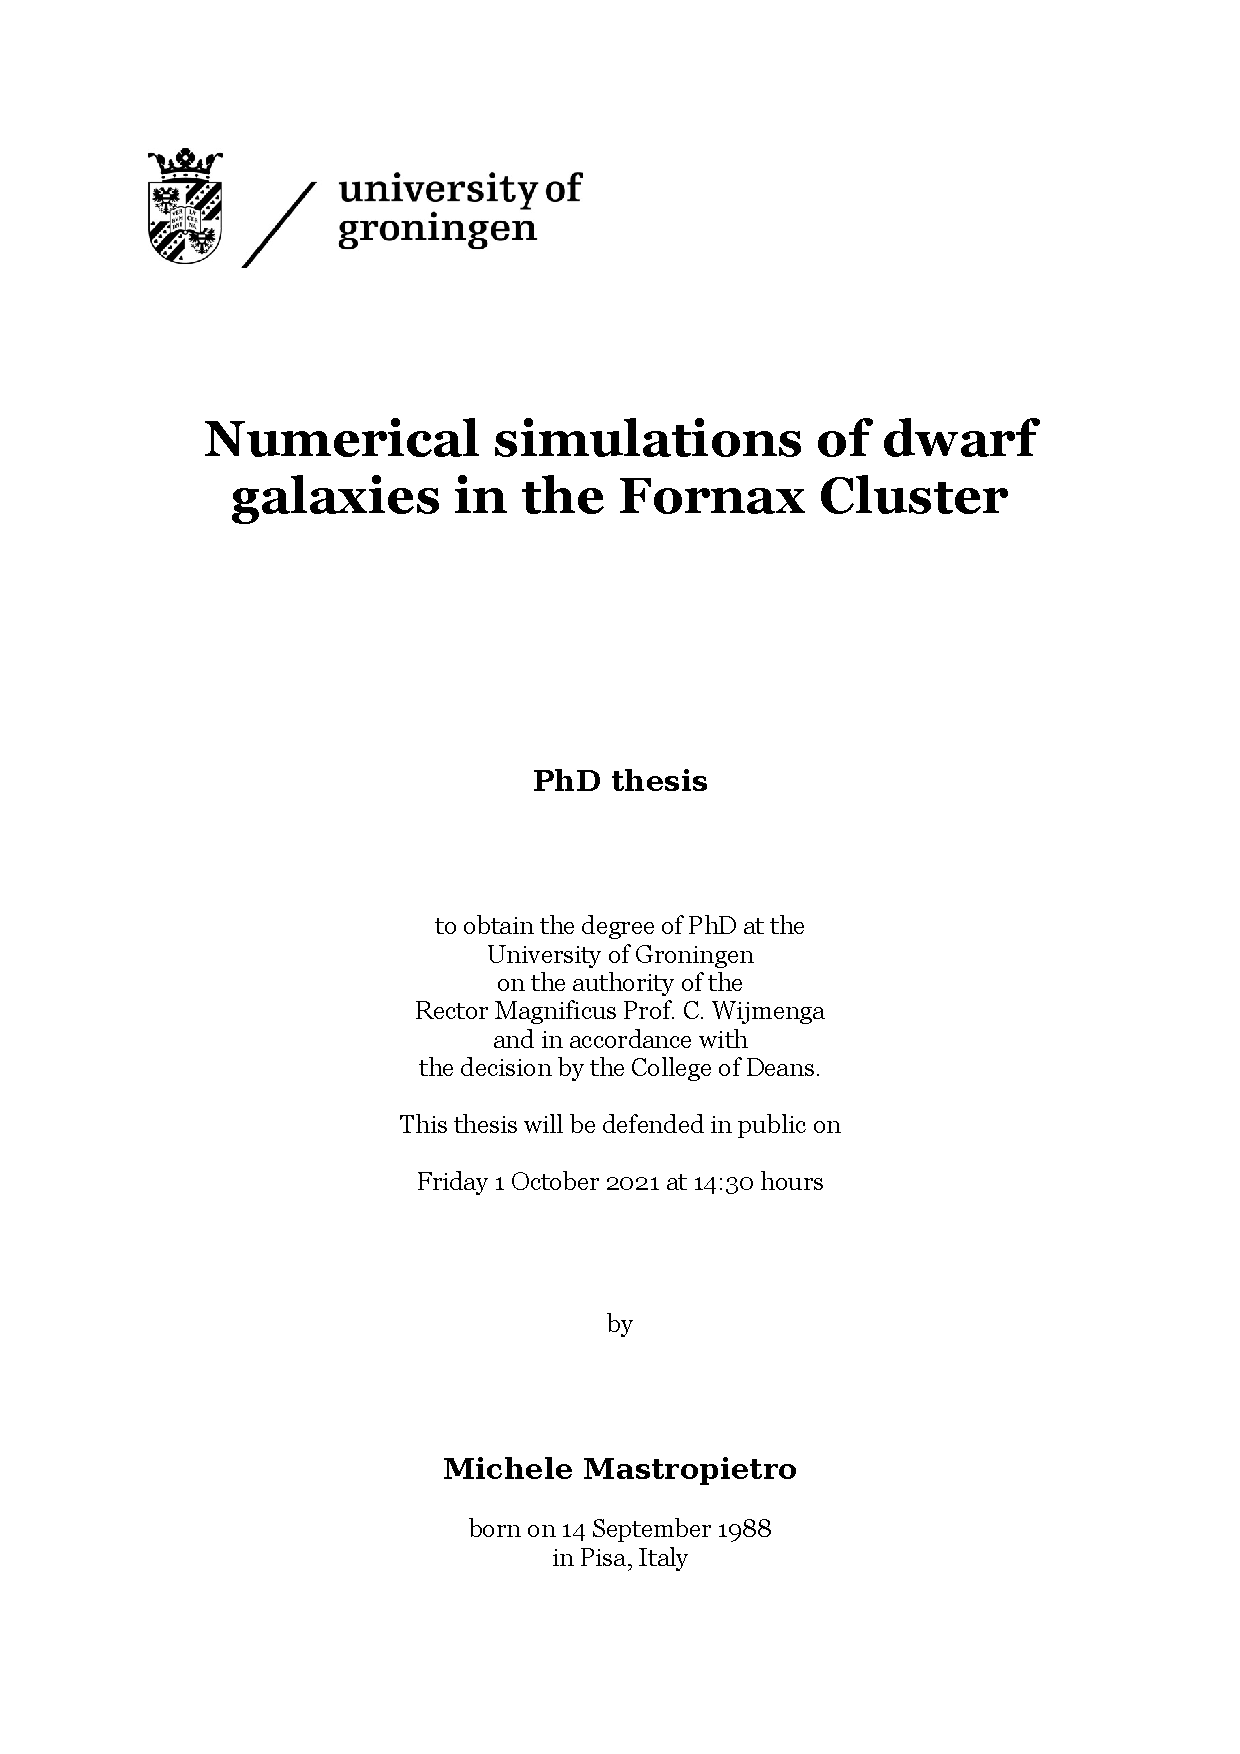
\includepdf[pages=-]{title_page.pdf}


\begin{comment}
% Official title
\begin{titlepage}
\null%
\label{thesis:title}
\vspace{3em}%
\pdfbookmark[1]{Title}{thesis:title}
\begin{center}

%% Skip space as in half-title
\vspace*{4\baselineskip}

%% Print the title.
\makeatletter
{\huge\@title}
\makeatother
\vfill

{\Large Proefschrift}

\medskip

{voorgedragen tot het behalen van \\
de graad van
Doctor in de Fysica en Sterrenkunde}


\medskip

door

\medskip

\makeatletter
{\Large \@author}
\makeatother

\medskip

aan de\\
{\large Universiteit Gent}\\
en aan de\\
{\large Rijksuniversiteit Groningen}\\
% Graduate School of Science and Engineering\\

\end{center}
\end{titlepage}





% Official verso
\clearpage
\thispagestyle{empty}
\null%
\label{thesis:committee}
\vfill
\pdfbookmark[1]{Doctoral committee}{thesis:committee}

% \noindent Members of the examination board:

\medskip\noindent
\begin{tabular}{@{}lll@{}}{Promotors:}\\\\
  \quad{}Prof.\ dr. Sven De Rijcke & Ghent University & (promotor)\\
  \quad{}Prof.\ dr. Michael\ Biehl & University of Groningen & (promotor)\\
  \quad{}Prof.\ dr. Reynier\ Peletier & University of Groningen & (promotor)\\
\\\\
\multicolumn{2}{@{}l@{}}{Composition of the Joint Evaluation Committee:} \\
\\
%   \quad{}Prof.\ dr.\  & chairperson \\
   \quad{}Prof.\ dr.\ Frazer Pearce & University of Nottingham\\
   \quad{}Prof.\ dr.\ Arjen van der Wel & Ghent University \\
   \quad{}Prof.\ dr.\ John McKean & University of Groningen \\
   \quad{}Prof.\ dr.\ Hugues Talbot & Université Paris-Saclay\\
\medskip\noindent
%   \quad{}Dr.\ & University of Groningen\\
% \\
% \multicolumn{2}{@{}l@{}}{Independent members:} \\
% \\
%   \quad{}Prof.\ dr.\ & University of Technology \\
%   \quad{}Prof.\ dr.\ & University \\
%   \quad{}Dr.\& University \\
% \\
% \multicolumn{2}{@{}l@{}}{Other member:} \\
% \\
%   \quad{}Dr.\ & ...\\
\end{tabular}
\end{comment}



% Copyright page
\clearpage
\thispagestyle{empty}
\null%
\label{thesis:colophon}
\vfill
\pdfbookmark[1]{Colophon}{thesis:colophon}
\noindent Written in 2021 by {\makeatletter{\@author}\makeatother}.\\
\textbf{Copyright}~\cczero{} The template for the layout of this thesis was inspired by my colleague Sam Verstocken who used the template of the dissertation of \href{ken.mx}{Ken Arroyo Ohori},
which was released into the public domain using the Creative~Commons~\cczero{}~code.
To view a copy of the \cczero{}~code, visit:\\\url{http://creativecommons.org/publicdomain/zero/1.0/}\\
\textbf{Colophon}
% This thesis was typeset with \XeTeX, Version 3.14159265-2.6-0.99998 (TeX Live 2017/Debian) using the \mbox{{\fanciestfont{}Feijoa}}, \texttt{GT Pressura} and $\mathrm{Asana\ Math}$ typefaces.
Most of the figures were created using \href{http://ipe.otfried.org/}{Ipe} (Copyright © 1993–2020 Otfried Cheong).
The source code of this thesis is available at: \\
\url{https://github.com/elehcim/phd-thesis}\\
\textbf{Cover}
...\\[2ex]
This research was funded by the European Union's Horizon 2020 research and innovation programme under the Marie Sk\l odowska-Curie
% Skłodowska-Curie
grant agreement N.~721463 to the \href{www.astro.rug.nl/~sundial}{SUNDIAL ITN network}.
\begin{figure*}[bh!]
  \centering
  
\includegraphics[width=0.2\textwidth]{EUflag}
\end{figure*}

% Aknowledgements page
\clearpage
\thispagestyle{empty}
\null%
\vfill
\begin{flushright}
  \textit{To my professor of physics:\\
      Mauro dell'Orso\\
      }
\end{flushright}
\vfill

% Aknowledgements page
\clearpage
\thispagestyle{empty}
\null%
\label{thesis:acknowledgements}
  \begin{center}
    {\Large \textbf{Acknowledgements}}\\
  \end{center}
\pdfbookmark[1]{Acknowledgements}{thesis:acknowledgements}
I'd like to thank first of all my professor Sven De Rijcke who believed in me doing a PhD in physics, since the first email in February 2017.
I thank you Sven for showing me what science is, how can it be beautiful and difficult and how it is a fantastic gym to train in deep honesty and integrity.
%As Feynmann said: we've learned from experience that the truth will come out, and it's this type of integrity, this kind of care not to fool yourself.
I've learned from you how to cope with work and life difficulties (especially in these pandemic times) in a very mature and ironic way.
Thank you also for being a mirror for me in our meetings, and always pushing me up even in my down moments.

The SUNDIAL project has been one of the nicest group of people I've ever met.
I'll never forget the high quality of people, their professionalism, attention and kindness for all of us. Thanks to prof. Michael Biehl, for your availability in this joint PhD journey.
Thank you prof. Reynier Peletier, our PI, practically a supervisor for all of us, always available to investigate new ideas with frank and direct attitude: %despite the many obligations and meetings you had to attend:
it's been very inspiring seeing how you live education of young scientists and astronomical research as a calling.
%Thank you Johan, my external mentor, for the interest you showed in my, for being kind and firm showing me how to clearly express.
Thanks to all of the ESRs, the one I had to work directly with: Marco, Abol, Bahar, and each one of the others: Maria Angela, Caroline, Aleke, Alex, Teymoor, Thanh, Mohammad, Shiv, Nushkia, Alan. All the best with your future.
The collaboration among us ESRs has often ended up in very good friendships, and I'll always remember the many memorable moments we lived together (in Naples, La Palma, Ghent...).

I thank my fellow astronomer colleagues at S9, the ones who are there, the ones who left during these years and the ones who just arrived.
I've learned so much from you academically and also how nice and beneficial is a happy work environment like the one you created.
The Belgian ``old guard": Maarten, Seba, Wouter, Peter, Sam, Marjorie, Dries, Robbert, Bert, Ilse, fellow Bert. Thank you for being so welcoming.
Thanks to Ana and Goran for the many moments shared together in our common expats life. Thanks to Francesco and Martina and their family: I've learned so much from you in these years we both were in Gent, much more than you think.
Caro and Pablo, thank you for all the support, deep sharing and friendship.Thank you dear office mates: Caroline, Sara, Anand and Yolan for the discussions and the nice coffee and fruit breaks.
You all have been so nice towards me, it's been an honour to work in the same place as you. Thank you for the many parties, events and dinners and many nice moments lived together.
I also thank the group of the Maxwell Demons: nice people for playing minivoetbal with fantastic team spirit.
Thank you Daniela and Andrea, young fellows of survival in lockdown times: I had so many great moments with you.
Thank you Shivangee, companion of the SUNDIAL adventure, of the office and of the life in Ghent in the happy moments as well as in the difficult times of the PhD far from home: for your constant positive attitude and for always asking how was going on for me and carefully listening. It meant a lot for me.
Thanks to Gianmarco (Jimmy), for showing me many times what true friendship means, and for being at the same time guest and host in our house in Belgium which became yours.
I thank Angelos, a real ``Sam" for me, in the sense of the Lord of the Rings: many times helping me %bringing the sometimes heavy burden of the PhD
and pulling me out of my down moments with frank conversations (is it a perk of living in Frank Baurstraat? ;P), sharing deep insights about life, cooking delicious Greek food (with an appropriate amount of garlic) and being the fuel of many parties and gatherings, with a lot of attention to everyone.

Thanks to my friends at Sint Jacobs in Gent: Davide and Ana (with the newly arrived Bea), Maria and Esteban (with the newly arrived Jose), Caique and Daniela, Valeria, Joshi, Pawel, Eligio and Luca: thank you for the improvised dinners, beers, holidays and deep friendship.
Many thanks to Pinco and the community of the Apostoline for helping me in many ways in these years: thank you for your wisdom and the constant example of free giving (gratuità).

I thank my family: mamma e babbo, for your unbreakable, positive, caring attitude towards me.
%Mi stupisco spesso di come vi siate adattati a fare i genitori di persone adulte con i fatti mostrando una strada siate davvero i genitori che vorrei avere, in tutti questi anni.
Anto for the crystalline confrontations and the enormous sensitivity, Fra for the innumerable funny stories and deep thoughts. Nonna Lida per esserci ed essere una roccia salda per tutti, always.

%Looking back at these years and looking forward for what is waiting for me,
Now that the future opens up after this beautiful adventure of the PhD, I'm on the road to find out a good way to spend my life: each of you is invaluable for orienting me in this. Thank you!

\begin{flushright}
  Gent, 14th September 2021\\Michele Mastropietro
\end{flushright}

% Summary page
\clearpage
\thispagestyle{empty}
\null%
\label{thesis:Summary}
\begin{center}
  {\Large \textbf{Summary}}\\
\end{center}
\pdfbookmark[1]{Summary}{thesis:Summary}

Dwarf galaxies are the most numerous type of stellar systems in the Universe and due to their low mass, they are very sensitive to the surrounding environment.
Because of this, they offer a privileged platform to study and isolate the different physical phenomena affecting galaxy observables.
They can be used as probes to characterize the complex interplay between internal processes and the environment in which galaxies evolve.

We carried out simulations of the evolution of dwarf galaxies falling into a Fornax-like Cluster.
We selected prototypical dwarf galaxies from the MoRIA suite of simulations and injected them one by one on different orbits.
We were interested in following the journey of the galaxies into the cluster and characterize their size, star formation rate, gas and dark matter content, stellar dynamics and evolution, depending on the orbit and the initial mass at the time of orbital injection.
To do so, we implemented the Moving Box simulation technique in our in-house simulation code.
This allows us to simulate the dwarf-cluster interaction at high resolution while keeping an affordable run time.

We found that during infall, generally, galaxies undergo some ``phase transition" happening mainly around pericenter passages.
Some of the galaxies are effectively transformed into Ultra Diffuse Galaxies (UDG) while some others are allowed to be briefly identified as ``jellyfish".
It is therefore possible to hypothesize that the jellyfish phenomenon is a relatively short transitory phase of a dwarf galaxy along its orbit, and it's likely a precursor of the transformation of a dwarf galaxy into an UDG.

Serendipitously we realized that our simulations produce galaxies whose morphology is similar to a galaxy in the Fornax Cluster with a peculiar  \Hi{} tail and an arrow-shaped stellar body oriented in different directions: NGC~1427A.
Multiple formation scenarios have been proposed for this galaxy, but a consensus was still lacking in the literature.
We identified that gaseous and stellar tails pointing in different directions are explainable given that they are subject to different environmental effects (ram-pressure stripping and tidal forces). This idea finds support in our simulations and we developed a procedure to quantitatively assess the properties of simulated galaxies from a catalogue of simulations.
We were also able to provide some falsifiable predictions on the position of the galaxy with respect to the center of the Cluster and its projected orbital direction.

Finally, we have contributed to the development of a technique to study low dimensional-manifolds in the simulations.
We found that the technique can be very useful to isolate the physical properties of filaments in N-body simulations.
In particular we concentrated on the analysis of gaseous tails of simulated jellyfish galaxies with the aim of investigating regions of recent star formation and mixing between the galactic gaseous material and the hot gas of the cluster.


\clearpage
\thispagestyle{empty}
\null%
\begin{center}
  {\Large \textbf{Samenvatting}}\\
\end{center}

%\begin{otherlanguage*}{dutch}
Dwerggalaxieën zijn het talrijkste type sterrenstelsels in het heelal en door hun lage massa zijn zij zeer gevoelig voor hun omgeving.
Daarom bieden zij een bevoorrecht platform om de verschillende fysische fenomenen die de waarneembare eigenschappen van sterrenstelsels beïnvloeden, te bestuderen en te isoleren.
Ze kunnen worden gebruikt als laboratoria om de complexe wisselwerking tussen interne processen en de omgeving waarin galaxieën evolueren te onderzoeken en te karakteriseren.

Wij hebben simulaties uitgevoerd van de evolutie van verschillende dwerggalaxieën die in een Fornax-achtige Cluster vallen.
We selecteerden prototypische dwerggalaxieën uit de MoRIA-simulatiesuite en injecteerden ze één voor één op verschillende banen.
We waren geïnteresseerd in het volgen van de reis van de melkwegstelsels in de cluster en het karakteriseren van hun grootte, stervormingssnelheden, hun inhoud aan gas en donkere materie, hun interne dynamica en hun evolutie, afhankelijk van de baan en de initiële massa op het moment van de injectie in de baan.
Daartoe hebben wij de Moving-Box-simulatietechniek aangepast aan onze noden en geïmplementeerd in onze eigen simulatiecode.
Dit maakt het mogelijk om de dwerg-clusterinteractie met zeer hoge resolutie te simuleren binnen een haalbare totale runtijd.

We ontdekten dat tijdens de inval, over het algemeen, melkwegstelsels enkele faseovergangen ondergaan, die voornamelijk  plaatsvinden bij pericenterpassages.
Sommige van de stelsels  worden getransformeerd in Ultra Diffuse Galaxies (UDG), andere worden kortstondig geïdentificeerd als ``jellyfish''.
Het is daarom mogelijk te veronderstellen dat het ``jellyfish"-fenomeen een relatief korte overgangsfase is van een dwergmelkwegstelsel langs zijn baan, en waarschijnlijk een voorloper is van de transformatie van een dwerggalaxie in een UDG.

Dankzij enige serendipiteit realiseerden we ons dat onze simulaties melkwegstelsels produceren waarvan de morfologie vergelijkbaar is met die van een welbepaald melkwegstelsel in de Fornax Cluster met een eigenaardige  \Hi{} staart en een pijlvormig stellair lichaam die in verschillende richtingen georiënteerd zijn: NGC~1427A.
Voor dit sterrenstelsel zijn meerdere formatiescenario's voorgesteld, maar in de literatuur was er nog geen consensus over.
Wij stelden vast dat gasvormige en stellaire staarten die in verschillende richtingen wijzen verklaarbaar zijn, aangezien zij onderhevig zijn aan verschillende omgevingseffecten (ramdruk en getijdekrachten).
Dit wordt ondersteund door onze simulaties en wij hebben een procedure ontwikkeld om de eigenschappen van gesimuleerde melkwegstelsels kwantitatief te beoordelen aan de hand van een catalogus van simulaties.
We waren ook in staat om enkele falsifieerbare voorspellingen te doen over de positie van het melkwegstelsel ten opzichte van het centrum van de Cluster en zijn geprojecteerde baanrichting.

Tenslotte hebben we bijgedragen aan de ontwikkeling van een techniek om laagdimensionale manifolds in simulaties de bestuderen.
We ontdekten dat de techniek zeer nuttig kan zijn om de fysische eigenschappen van filamenten in N-body-simulaties te isoleren.
In het bijzonder hebben we ons geconcentreerd op de analyse van gasvormige staarten van gesimuleerde ``jellyfish"-sterrenstelsels met het doel regio's van recente stervorming en vermenging tussen het galactische gasachtige materiaal en het hete gas van de cluster te onderzoeken.
%\end{otherlanguage*}

\clearpage
\thispagestyle{empty}
\null%
\begin{center}
  {\Large \textbf{Riassunto}}\\
\end{center}
\begin{otherlanguage*}{italian}
Le galassie nane sono i sistemi stellari più numerosi dell'Universo e, a causa della loro piccola massa, sono molto sensibili all'ambiente che sta loro intorno.
Per questo motivo, offrono una piattaforma privilegiata per studiare e isolare i diversi fenomeni fisici che influenzano le caratteristiche osservabili delle galassie.
Possono essere utilizzati come sonde per caratterizzare la complessa interazione tra i processi interni e l'ambiente in cui le galassie si evolvono.

Abbiamo effettuato simulazioni dell'evoluzione delle galassie nane che cadono in un ammasso con caratteristiche simili a quello della Fornace.
Con alcune galassie prototipali selezionate dalla suite di simulazioni MoRIA e abbiamo messe su una per una su diverse orbite.
È di interesse scientifico seguire il viaggio delle galassie nell'ammasso e a caratterizzare le loro dimensioni, la formazione stellare, il contenuto di gas e materia oscura, la dinamica stellare e la sua evoluzione, a seconda dell'orbita e della massa iniziale al momento dell'iniezione orbitale.
Per fare ciò, abbiamo implementato la tecnica di simulazione chiamata ``Moving Box" nel codice sviluppato nel nostro dipartimento.
Questo ci ha permetto di simulare l'interazione galassia nana ammasso ad alta risoluzione mantenendo un pratico tempo di calcolo.

Abbiamo trovato che durante l'orbita, generalmente, le galassie subiscono alcune ``transizioni di fase" che avvengono principalmente attorno al passaggio per il pericentro.
Alcune galassie vengono effettivamente trasformate in Galassie Ultra Diffuse (UDG), mentre altre possono essere identificate brevemente come ``galassie medusa'' (jellifish).
È quindi possibile ipotizzare che il fenomeno delle galassie medusa sia una fase transitoria relativamente breve di una galassia nana lungo la sua orbita, e che constituisca probabilmente un precursore della trasformazione di una galassia nana in una UDG.

Per una fortuita combinazione, abbiamo notato che le nostre simulazioni producono galassie la cui morfologia è simile a quella di una galassia dell'ammasso della Fornace con una peculiare coda \Hi{} e un corpo stellare a forma di freccia, orientate in diverse direzioni: la NGC~1427A.
Per questa galassia sono stati proposti molteplici scenari di formazione, ma manca ancora un consenso in letteratura.
Abbiamo identificato che le code gassose e stellari che puntano in direzioni diverse sono spiegabili dato che ognuna è soggetta a diversi effetti ambientali (pressione e forze di marea).
Questa idea trova supporto nelle nostre simulazioni.
Abbiamo quindi sviluppato una procedura per valutare quantitativamente le proprietà delle galassie simulate partendo da un catalogo di simulazioni.
Siamo stati anche in grado di fornire alcune previsioni falsificabili sulla posizione della galassia rispetto al centro dell'ammasso e la sua direzione orbitale proiettata.

Infine, abbiamo contribuito allo sviluppo di una tecnica per studiare nelle simulazioni le varietà (manifold) con una dimensionalità bassa.
Abbiamo scoperto che questa tecnica può essere molto utile per isolare le proprietà fisiche dei filamenti nelle simulazioni a N corpi.
In particolare, ci siamo concentrati sull'analisi delle code gassose delle galassie medusa simulate con l'obiettivo di indagare le regioni di recente formazione stellare e di mescolamento tra il materiale gassoso galattico e il gas caldo dell'ammasso.
\end{otherlanguage*}

\cleardoublepage

\tableofcontents

% \listoffigures

% \listoftables


\mainmatter



% !TEX root = thesis.tex

\chapter{Introduction}
\label{ch:introduction}

The Dark Energy plus Cold Dark Matter (\lcdm{}) cosmological model is the current ``standard model" which satisfactorily reproduces the present-day observations of the large scale structure of the Universe, of the Cosmic Microwave Background (CMB) and of supernovae indicating an accelerating expansion of the Universe \citep{Riess1998}.
According to \lcdm{}, the Universe was formed $13.8$~Gyr ago, through the so called Big Bang, when the Universe was a hot plasma.
After a phase of sudden expansion, the consequent cooling allowed the radiation to decouple from the ordinary matter.
The last radiation scattered before the Universe became transparent is called the Cosmic Microwave Background and it is observable now in the microwave range as an uniformly distributed radiation of a black body of $2.7$~K.
Since black body spectra are produced by opaque objects CMB brings the information that the early Universe was opaque \citep{Ryden2003}.

However, at the beginning of the XX century, various measurements found that the amount of visible (baryonic) matter was not enough to justify observations of galaxy motion and their rotation.
\citet{Zwicky1933} first recognized the discrepancy and the missing matter by observing the rotation velocity of the galaxies in the outskirts of the Coma cluster \citep{Zwicky1937}.
He therefore hypothesized the existence of dark matter, a kind of matter which does not interact with the electromagnetic forces but only with gravity.
%Later observations confirmed that the missing mass could be accounted for from the rotation curves from galaxies %TODO(Babcock, 1939; Rubin & Ford, 1970; Bosma, 1978; Rubin et al., 1980).
All these observations showed that in the Universe, the amount of dark matter is around five to six times more than baryonic matter.
Another observational fact coming from supernovae, is the accelerating expansion of the Universe.
The current accepted model is the presence of an large scale unknown form of energy, called Dark Energy (or $\Lambda$), which constitutes around 68\% of al the mass-energy content of the Universe.
The \lcdm{} model also assumes that the dark matter is ``cold", \ie{} it has negligible thermal velocity and does not suppress structure formation on any scale relevant for galaxy formation \citep{Bullock2017}.
Baryonic and dark matter gravitationally collapsing slowly formed filaments along which gas could become dense enough to create self-supporting gravitational systems cradle of stars, the first galaxies.
These filaments have been observed in large surveys like the Sloan Digital Sky Survey (SDSS). % TODO figure here?

The study of galaxies has seen its development only very recently.
Less than one century ago, current recognized galaxies were thought to be small luminous clouds (and thus called \emph{nebulae}) belonging to our Galaxy, the Milky Way, the only known Galaxy.
In 1923 Edwin Hubble, measuring the distance of the \emph{nebulae} by observing their variable stars Cepheids, from the observatory of Mount Wilson in California, realized they were systems far away from the Galaxy \citep{Hubble1929}.
His observations have completely changed the view of the Universe.
The scientific research on galaxies took off from Hubble's works and even the morphological classification of galaxies took his name.

In this thesis we are particular interested in small galaxies, the so called \emph{dwarf galaxies}.
They are the most numerous type of stellar systems in the Universe and due to their low mass, they are very sensitive to the surrounding environment.
For this they offer a privileged platform to study and isolate the different physical phenomena affecting galaxies observables.
They can be used as probes to characterize the complex interplay between internal processes and the environment in which they evolve.

%Using high definition hydrodynamical simulations, we investigate the evolution of dwarf galaxies falling into the Fornax cluster.

%We have carried out a representative set of simulations putting MoRIA dwarfs with stellar masses in the range of 4e6 - 1e9 Msol on infalling trajectories with different pericenter distances.
%We find that the combined effect of tidal interactions and ram-pressure for late-type dwarf galaxies can produce strong star burst episodes during pericenter passages followed by quenched star formation. Also, star forming galaxy tails (jellyfish galaxies) are observed. We find that dwarfs within this mass range that are on very radial orbits do not survive up to z=0. We also show the results of the analysis of the simulations following the dwarfs' journey

\section{Falling into a galaxy cluster}

The evolution of galaxies in dense environments has been shown to be markedly different from that of more isolated galaxies, with mass being a prominent factor in determining how profoundly environmental influences affect a galaxy \citep{Boselli2006, Grossi2018a}.
The well-known morphology-density relation, according to which early-type galaxies are mostly found in high-density environments \citep{Dressler1980, Dressler1997}, is especially pronounced for low-mass systems, such as dwarf galaxies \citep{McConnachie2012}.
Indeed, while actively star-forming late-type dwarf galaxies are found almost exclusively in low-density environments, truly isolated quiescent early-type dwarf galaxies, on the contrary, are exceedingly rare \citep{Binggeli1990, Karachentseva2010, Geha2012}.

An effective way of shutting down the star formation in a galaxy is to rob it of the raw material for building stars:~gas.
When a galaxy enters on an orbit in a galaxy cluster or group, it is subjected to the tidal forces of the cluster potential and of its galaxies.
Its interstellar medium experiences the ram pressure \citep{GunnGott1972}, basically a supersonic ``headwind", exerted by the intracluster medium.
Ram pressure is a well known phenomenon and many studies have been devoted to simulating its effects on galaxies \citep[e.g.:][]{Mori2000, Mayer2006, Roediger2008, Roediger2015, Steinhauser2016, Yun2018, Steyrleithner2020}.
If the ram pressure is sufficiently vigorous, the galaxy's diffuse interstellar medium can be pushed out of its gravitational well, forming a tail of escaping \Hi{} gas in the galaxy's wake.
The much more clumpy molecular gas is not as easily removed by the ram pressure and remains behind while being consumed by star formation \citep{Abramson2014, Lee2017, Wang2020}.
Inside the tail, gas can cool and form knotty condensations, leading to a complex stellar system, with a head consisting of the galaxy's stellar body (and what remains of its gas) and a tail of twisting swirls of stripped gas, beaded with knots of star formation.

The term \emph{jellyfish galaxies} \citep{Ebeling2013} neatly fits this description. %and hence they are prime candidates for interpreting the transformation processes acting on galaxies in cluster and group environments.
The term applies to galaxies with star formation activity within the gaseous tails.
Jellyfish galaxies exhibit tentacles of material that appear to be stripped from the galaxy body \citep{Poggianti2017a, Poggianti2019b, Ramatsoku2020}.
Signatures of the newly born stars within those gaseous tails are easily found observationally in UV or blue images \citep{Cortese2007,Smith2010a}.
\bigskip

%\subsubsection{Other works}
As already noted by many authors \citep{Mayer2001, Mayer2007, Mastropietro2005} %FIXME maybe also somebody more recent?
ram pressure stripping \citep{GunnGott1972, Roediger2008, Roediger2015} and tidal interaction can cooperate to change the morphology of the galaxy.
Recent studies using cosmological simulations deal with dwarf galaxies infalling into a galaxy cluster.
\citet{Smith2015} evolve a large population of early type galaxies and take into account tidal interactions and harassment effects but with no gas physics.
%We argue that this can have a non negligible effects when trying to follow the evolution of observables like effective radius, gas distribution, stellar kinematics, age and metallicity gradients.


Using the cosmological simulation TNG100, \citet{Yun2018} visually inspect infalling galaxies in simulated clusters to characterise jellyfish galaxies.
%but the galaxies considered start from $10^9.5$ \Msun{} which is our upper limit of the dwarfs we simulate.
Interestingly, they also found a dearth of jellyfish galaxies within one fourth of the cluster virial radius.
This is consistent with current catalogues of cluster galaxies \citep{Lisker2006, Venhola2019}.

% \section{Late-type to early-type conversion??}
%Dwarfs falling into a hot dense halo undergo ram pressure stripping which remove the cold gas reservoir and their possibility to form stars.
%In addition, tidal interactions make their potential shallower and, in turn, removal of the gas is enhanced.
%This results in the well-known morphology-density relation, according to which early-type galaxies are mostly found in high-density environments \citep{Dressler1980, Dressler1997}. The relation is even more noticeable in dwarf galaxies \citep{McConnachie2012}.

\citet{DeRijcke2010}, from dynamical models of the Fornax Cluster as a whole, could explain the radially increasing late-to-early-type dwarf ratio in the cluster.
In the Virgo cluster, \citet{Boselli2008} highlights that low mass galaxy at the first infall lose most of their \Hi{} and are quenched.
After, these objects become red and quiescent.
\citet{Ruggiero2017}, using \textsc{Ramses} simulations constrain how much of the gas disc of a Milky Way like galaxy will be converted into stars and how much of it will be lost, after a single cluster crossing.
They find star formation bursts on infall and remark that the survival of the galaxy is independent on the galaxy orbit and cluster mass if the cluster has a cool core.
The removal of the gas has been studied for example by \cite{Calura2020} who follow the evolution of a massive pressure-confined, star-forming neutral gas cloud moving through a hot intracluster medium (ICM).
They find that generally cold clouds survive with a final cold gas fractions generally greater than 0.75 on time-scales of the order of 1 Gyr.
But while the removal of cold gas is a quick process (a time scale $\leq$1 Gyr), a few Gyr are required to quench the galaxy and reach the red sequence \citep{Cortese2009}.

% \citet{Hausammann2019}

\citet{Venhola2018} show that number density of dwarfs in the Fornax cluster decreases going towards the centre of the cluster.
A possible scenario suggests that some infalling galaxies do not survive in the passage around the centre of the cluster.
Further investigation is needed to assess  whether the disrupted galaxies then contribute to the Intra-Cluster Light (ICL) or become Ultra Diffuse Galaxies (UDG).
Trying to shed light on how easily dwarfs are being dissolved around cluster centre and comparing the simulation output with recent and ongoing surveys such as the SAMI High Resolution Survey of Fornax Dwarf Galaxies, \citep{Owers2019, Scott2018}
the Fornax Deep Survey \citep{Venhola2018}, and the Fornax MeerKAT survey \citep{Loni2021} is one of the motivations for this work.



\begin{figure}
  \centering
  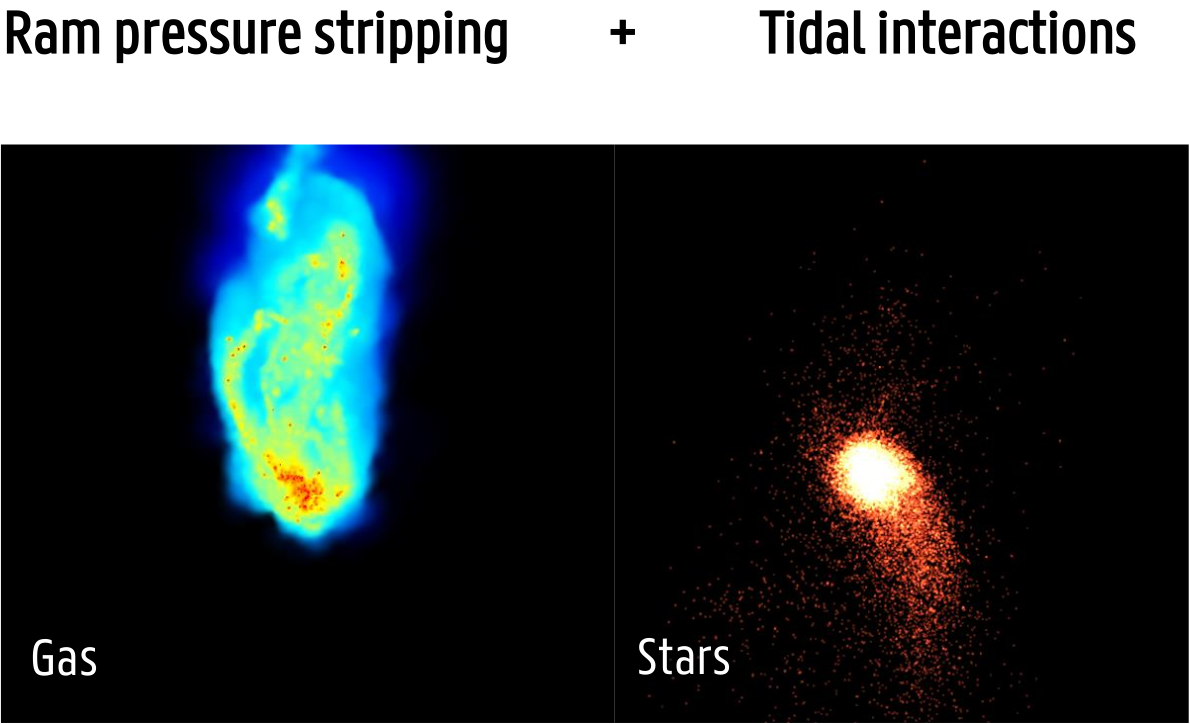
\includegraphics[width=\textwidth]{Gas_Tails}
  \caption{On the left the gaseous component of a simulated dwarf galaxy, color coded with projected density.
    On the right the stellar particles of the same galaxy.
   Different physical processes (of ram pressure stripping and tidal interactions) affecting the galaxy can lead to the creation of the curious effect of gaseous and stellar tails oriented in almost opposite directions.}
  \label{fig:tails}
\end{figure}


\section{This work}
To the best of our knowledge our work is the first to apply the Moving Box technique (see Section~\ref{sec:MovingBox}) to a galaxy cluster setup, using high definition simulations.
In comparison to earlier work our simulations take into account gas-rich realistic late type galaxies. To our knowledge none of them include such a high definition simulation starting from with late-type dwarfs models.


% !TEX root = thesis.tex

\chapter{Simulations}
\label{ch:simulations}

Numerical simulations have emerged as a new tool to investigate nature, alongside theory and experiments.
This is particularly valid for astronomy where, unlike laboratory-based disciplines, astronomers may not exert full control over their study objects \citep{Heng2014}.

Computer simulations are essentially a tools to solve complex systems of equations which are intractable with analytic techniques, or only tractable with very coarse level of approximation \citep{Springel2015}.
This allows an unprecedentedly detailed exploration of the consequences of assumed models for physical systems.
In this sense, the reproduction of observations through computer simulations is a way to validate scientific hypotheses.
The main mathematical model used in galaxy simulations is the fluid model, a branch of continuum mechanics which deals with materials represented as continuous mass as opposed to discrete particles.
In fact, we are not interested in the motion of each molecule in detail, rather we will use a statistical approach.
In the following we will be dealing with hydrodynamics, given that the main components of galaxies are successfully described in terms of fluids.

\section{General assumptions}
We will assume the Cold Dark Matter (CMD) paradigm (in a $\Lambda$CDM cosmology), which has gained consensus among the scientific community throughout the years even if up to now, there has been no detection of it \citep[see e.g.][for an extensive and historical overview]{Einasto2010}.
In a dwarf galaxy simulation three kind of fluids are generally taken into account, each following different models: dark matter, gas and star. The latter two are so called \emph{baryonic} matter.

Dark matter is hypothesized to consist of small particles that are orders of magnitude smaller than the typical distance scales in our galaxies, so that they constitute a collisionless fluid.
Similarly, the cross section of stars is small compared to galactic scales, and makes them collisionless as well.
Stars, though, affect the gas by pumping energy and metals into their surroundings.
Dark matter and stars are therefore sensitive only to gravity, a weak, conservative, long-range force which is caused by a generally smooth potential.

On the other hand, as we shall see, gas is collisional and its behaviour at any point is affected by short-range interactions, whose modeling requires other assumptions (see below Sections \ref{sec:extended_gas_physics} and \ref{sec:dwarf_models}).

\subsection{Boltzmann Equation - Equations of motion}
The Boltzmann Equation is the general equation which governs the behaviour of a fluid.
From it, the equations of motions can be derived and solved to assess the evolution through time of the fluid.

For simplicity, in this section we assume a single-species fluid, a generalization to multiple species being straightforward.
For each point of the fluid we would like to know its position and velocity.
Following a statistical approach, at any given time $t$ we can write the distribution function
\begin{equation}
f(\vect x, \vect u, t)
\end{equation}
which describes the number of molecules lying withing a spatial volume $\dd[3]{\vect x}$ about $\vect x$ and with velocity lying in a velocity-space volume $\dd[3]{\vect u}$ about $\vect u$.
These elementary volumes $\dd[3]{\vect x}$ and $\dd[3]{\vect u}$ are finite volume elements which are large enough to contain a very large number of molecules and still small enough to be considered as infinitesimal when compared to macroscopic dimensions \citep{Huang1987}.
% The distribution function has We can therefore introduce the concept of elementary volume in the 6D phase space $(\vect x, \vect u)$.

% in the elementary volume distribution of the position and velocity of a typical particle
% by its distribution function $f(\vect x, \vect u, t)$ which represents the number density of fluid molecules in the 6D phase space $(\vect x, \vect u)$.
% By multiplying this function with the phase space volume element $\dd[3]{\vect x} \dd[3]{\vect u}$, we obtain the number of particles within this phase space volume element at a given time $t$.
The number density $n(\vect x, t)$ in physical space is obtained by integrating over all possible velocities at a position $\vect x$:
\begin{equation}
n(\vect x, t ) = \int f(\vect x, \vect u, t) \dd[3]{\vect u}.
\end{equation}
The spatial density is then simply $\rho(\vect x, t) = m_p\,n(\vect x, t)$, where $m_p$ is the mass of the elementary molecule of the fluid.
From this we can define an average value in the position space of a generic quantity $A(\vect x, \vect u, t)$:
\begin{equation}
 \label{eq:df_average}
 \mean A (\vect x, t) = \frac{1}{\rho(\vect x, t)}\int{A(\vect x, \vect u, t)\, m_p\, f(\vect x, \vect u, t) \dd[3] \vect u}
\end{equation}
It is useful to define the averaged (\emph{bulk}) velocity $\vect{v}$ as:
\begin{equation}
  \vect{v}(\vect x, t) \equiv \mean{\vect u}(\vect x, t) = \frac{1}{\rho(\vect x, t)}\int{\vect u(\vect x, \vect u, t)\, m_p\, f(\vect x, \vect u, t) \dd[3] \vect u}
\end{equation}
For each elementary spatial volume $\dd[3] \vect x$ we can write the local velocity as the sum: $\vect u = \vect{v} + \vect w$, where $\vect{v}$ is the average particle velocity and $\vect w$ a term corresponding to the random movement of the particle with respect to the bulk flow velocity.

Assuming that the microscopic particles do not collide, the number density in phase space is conserved in time, i.e. no particles are destroyed or created out of nothing in phase space.
This gives immediately the collisionless Boltzmann equation (a.k.a. Vlasov equation):
\begin{equation}
\label{eq:vlasov}
\dv{f}{t}(\vect x, \vect u, t) = \pdv{f}{t} + \vect u \pdv{f}{\vect x} + \vect a \pdv{f}{\vect u} = 0,
\end{equation}
where $\displaystyle \vect a = \dv{\vect u}{t}$ is the acceleration.

In the case of collisions, the Boltzmann equation is modified to:
\begin{equation}
\label{eq:boltzmann}
\dv{f}{t}(\vect x, \vect u, t) = \left.\dv{f}{t}\right|_c,
\end{equation}
where the right term represents discontinuous motion of molecules through phase space because of collisions.

\subsubsection{Euler's equations}
After computing the zeroth, first and second velocity moments of equation \eqref{eq:boltzmann} ---by multiplying by $m_p$, $m_p\vect u$ and $m_p\norm{\vect u}^2$ and by integrating over the entire velocity space--- it is possible to retrieve the equations of hydrodynamics (continuity, momentum and energy) \citep[][and \cite{Vandenbroucke2016} for an extended derivation]{Huang1987}.

In the following we make the assumption that collisions do not create or destroy molecules at a fixed position (they only shift them in velocity space), they conserve momentum and energy.
Consequently in the case of the continuity, momentum and energy equations the right-hand side of equation \eqref{eq:boltzmann} vanishes.
We also neglect diffusive terms (heat conduction and viscous stress tensor) which are often small compared to dynamical effects (an important exception though are shocks, for example).

The hydrodynamical equations (a.k.a. Euler equations) are therefore:
\begin{align}
\label{eq:euler}
 \dv{\rho}{t} &= \pdv{\rho}{t} + \vect{v} \vdot \grad \rho = - \rho \,\div \vect{v}, \nonumber\\
 \dv{\vect{v}}{t} &= \pdv{\vect{v}}{t} + \left(\vect{v} \vdot \grad\right) \vect{v}  = \vect a - \frac{\grad p}{\rho},\\
 \dv{\energy}{t} &= \pdv{\energy}{t} + \vect{v} \vdot \grad \energy = - \frac{p}{\rho} \div \vect{v}. \nonumber%\frac{\Gamma - \Lambda}{\rho}
\end{align}
% \begin{equation}
%   \begin{split}
%     \dv{\rho}{t} & + \rho \,\div \vect u = 0\\
%     \dv{\vect u}{t} &+ \frac{\grad p}{\rho} = - \vect a\\
%     \dv{\energy}{t} & + \frac{p}{\rho} \div \vect u = 0
%   \end{split}
% \qquad\qquad
%   \begin{split}
%     &\pdv{\rho}{t} + \grad(\rho \vect{v}) = 0\\
%     &\pdv{t}(\rho \vect{v}) + \grad(\rho\vect{v} \vect{v}^T + p) = 0\\
% 	&\pdv{t}(\rho e) + \grad (\rho e \vect{v} + p\vect{v}) = 0
%   \end{split}
% \end{equation}
where we defined the pressure as $$p(\vect x, t) = \rho \dfrac 1 3 \trace{(\vect w \vect w^T)} = \rho \dfrac 1 3 \norm{\vect w}^2,$$ assuming an isotropic medium, and the specific internal energy (internal energy per unit mass) as $$\energy(\vect x, t)=\dfrac 1 2 \norm{\vect w}^2.$$ % FIXME Check if this is true
These definitions implicitly fix an equation of state
\begin{equation}
\label{eq:simple_eos}
p = \frac 2 3 \rho \energy.
\end{equation}
Usually a more general equation of state is assumed $p = (\gamma - 1) \rho \energy$.
For a monoatomic gas: $\gamma = \dfrac{5}{3}$, so equation \eqref{eq:simple_eos} is returned.

Also, the internal energy is related to the temperature via the Boltzmann constants $k_B$:
\[ \energy = \frac {1}{\gamma - 1} \frac{k_B T}{m_p}.\]
For a monoatomic gas $\displaystyle \energy = \frac 3 2 \frac{k_B T}{m_p}$.

% $\Gamma$ and $\Lambda$...

Equations \eqref{eq:euler} describe the dynamics of a perfect monoatomic gas.

\subsection{Gravity}
%We introduce an external force in the Euler equations.
Acceleration in each phase-space position is due to the gravitational field.

In case of self-gravity the source of the acceleration field is the mass density $\rho(\vect x, t)$:
\begin{equation}
 \div \vect a = - 4 \pi \,G \, \rho(\vect x, t).
\end{equation}

The gravitational potential $\vect a = - \grad \Phi$ can therefore be found through the Poisson's equation:
\begin{equation}
 \label{eq:poisson}
 \laplacian \Phi(\vect x,t) = 4 \pi \,G \, \rho(\vect x, t).
\end{equation}

% It is evident how important is to obtain an accurate estimate of the density. We will show a possible technique in the following. %TODO add this.

\section{N-Body systems}
The direct numerical solution of the Boltzmann equation, a non-linear PDE in seven dimensions, is not feasible.
It is interesting to note that in this description the particles have basically completely vanished and have been replaced with a continuum fluid description.
In order to solve the Boltzmann equation (or equivalently the Euler's equations), we represent the fluid by $N$ mass elements (particles), that are conceptually different from the microscopic particles (molecules) constituting the fluid.
The main idea is to discretize the equations above introducing particles.
These are therefore fiducial macro particles that sample the phase-space in a Monte-Carlo fashion \citep{Springel2015}.
Thus, in practice an $N$-body method is a tool for solving the Boltzmann equation.
% In this way then it reduces to solving the gravitational interactions for this $N$-body system \citep{Dehnem2011}.

The equation of motion for particles, following equations \eqref{eq:poisson} can be written as follows:
\begin{equation}
 \vect a_i = -\nabla_i \Phi(\vect x_i),
\end{equation}
\begin{equation}
 \Phi(\vect x_i) = -G \sum^N_{j=1}\frac{m_j}{\sqrt{(\vect x_i-\vect x_j)^2 + \epsilon^2}}.
\end{equation}

where we introduced the softening length $\epsilon$, effectively using a Plummer sphere potential for each particle \citep{Plummer1911}.
It's worthwhile to note, though, that particles interact with each other as a point mass and a Plummer potential, not as Plummer spheres with each other.

The purpose of the force softening is to avoid the numerical expense that would be needed to integrate the orbits with sufficient accuracy around the singularity in the $\sim 1/r$ potential.
Also, if two particles get very close their gravitational attraction will explode, leading to the possibility of the formation of bound particle pairs, strongly violating the collisionless behaviour.
The softening length is also called force resolution because we cannot resolve gravitational forces below that distance.
The value of the gravitational resolution is important when trying to follow the collapse of dense gas clouds where star formation is about to occur, as we shall see in Section~\ref{sec:star_formation}.
In our simulations we use a softening length of $\epsilon=30$~pc.
An estimate of this smoothing length is obtained by requiring that in the simulated gas clouds with the highest density, $\epsilon$ is about equal to the average distance between the gas particles \citep{Schroyen2013}. % Mail Sven 24/11/2017
Given that in the densest gas clouds star formation occurs at a density of $n\approx100$~amu/cm$^{3}$, when a galaxy is simulated with gas particles of $4000$~\Msun{}, the average distance between the particles in that gas cloud will be of the order of $11$~pc.

As \citet{Bate1997} and \citet{Springel2005} discuss, in order for SPH to produce the correct results in problems involving self-gravity, the hydrodynamic smoothing length and gravitational softening length must always be less than the local \emph{Jeans length} (see \refsec{sec:star_formation}). However, a gravitational softening much smaller than the SPH smoothing length can lead to artificial convergence of SPH particles.
This can be avoided if the force resolution is greater than the hydrodynamical resolution at the scale of high density clumps.

\section{Smoothed Particles Hydrodynamics}\label{sec:SPH}
Smoothed Particles Hydrodynamics (SPH) is a finite volume, Lagrangian particle based numerical method to solve the Navier-Stokes equation of motions for a fluid.
It is a Lagrangian method because the elements carrying information about the fluid move along the fluid itself.
% It is finite volume because it.

A different approach to discretize the fluid domain is to use an Eulerian approach, like grid based Adaptive Mesh Refinement (AMR).
Recently, so called \emph{moving-mesh} methods have emerged. They combine both approaches and are more flexible but come with their own difficulties \citep{Springel2010, Shadowfax, Arepo}.
% Several research groups are pushing forward different techniques, sometimes following their own tradition and claiming.
Usually simple test problems (Sod tube, Sedov blast-wave \citep{Sedov1946}, Kelvin-Helmholtz instabilities, Noh test \citep{Noh1987}, Gresho vortex \citep{Gresho1990}),
which can be solved analytically, serve as a benchmark for the accuracy of the numerical solution, \citep[e.g. by measuring the distance of the two solution with an L2-norm in the whole domain, ][]{BorrowSphenix}.
Numerical solutions are always a trade-off between accuracy and practicality.
It is interesting to see how a certain gain in accuracy is translated in an increase of \emph{time-to-solution} \citep{Borrow2019}.
%But at the end of the day if we pay attention to the the trend is

\subsection{Density Estimation from particles ensemble}\label{sec:density_estimation}
%\paragraph{Origin of SPH}
SPH has been originally developed as a \emph{probabilistic} particle method for simulating astrophysical problems \citep{Lucy1977, Gingold1977, Monaghan2005}\footnote{In a lecture given at Monash University in 2018 \url{https://youtu.be/tAXHCAEgSuE}, prof. Monaghan retraces the origin of the SPH method, recalling that the inspiration for the particle methods to estimate density in fluids comes from David George Kendall, a statistician he collaborated with in Cambridge.}.

The main idea of the SPH formalism is to write the equation of motion of the fluid for the sampling particles, solve them and then computed physical quantities in every point of the domain trough the so called \emph{SPH interpolation}.

This kind of interpolation is the same as the one used for the calculation of probability distributions from samples \citep{parzen1962estimation, 5178637}.
Given a kernel $W(x, h)$ function of the spatial coordinate $x$ with smoothing length $h$, the interpolation $A_I(\vect{r})$ of a quantity $A(\vect{r})$ is given by:
\begin{equation}
  A_I(\vect{r}) = \int A(\vect{r}') W(\norm{\vect{r} - \vect{r}'},h) \dd\vect{r}'.
  \label{eq:sph_interpolation}
\end{equation}
Any function which follow these two assumptions can be used as the smoothing kernel:
\begin{align*}
  \lim_{h\rightarrow 0} W(x, h) &= \delta(x),\\
  \int_{-\infty}^\infty W(x, h)\, \dd x &= 1
\end{align*}

%If we choose $W=\delta$, a delta function, then $A_I=A$.
%In practice, the kernels tend to the delta function as the smoothing length $h$ goes to zero.
An example of the kernel is a Gaussian:
\begin{equation}
  W(x, h) = \frac{1}{h\sqrt{\pi}} e^{-x^2/h^2}
\end{equation}

% In his original treatment \citet{Gingold1977} the probabilities of ... were defined as the expected value
% \begin{equation}
%  E[\rho] = ...% TODO expected values
% \end{equation}

% From J. Monaghan https://www.youtube.com/watch?v=tAXHCAEgSuE
% The general procedure of SPH for solving equations is:
% \begin{itemize}
%  \item Replace the continuum by particles
%  \item Calculate forces on particles
%  \item Follow the motion of the particles
% \end{itemize}
% In statistics the basic interpolant is used to compute probability density except that they do not have mass.
% Instead, for $N$ samples they have the factor $\frac 1 N$.


% Cambridge David Kendall professor of statistics they wanted to calculate probability distributions from samples. They use the same kind of interpolation.

% Problems: Accessing particles (if you have gravity the tree that you build to compute distances and gravity interactions between all the particles can be used in hydrodinamics too.
% The hydro differential equations become a set of ordinary differential equations and (t42:00) and a way to  timestepping is needed.
% Try to construct your discretized equations in a way that it contains the conservation properties of the continuum.


%A possible choice for the kernel is a Gaussian.
In general, it's much more practical to use a finite support approximation of a Gaussian.
The most often used for SPH are the Schoenberg  B-spline functions \citep{Schoenberg1946}, generated as the Fourier transform \citep{Monaghan1985, Monaghan2005, Price2012}:
\begin{equation}
M_n(r, h) = \frac{1}{2\pi}\int_{-\infty}^{\infty}{\left(\frac{\sin(kh/2)}{kh/2}\right)^n\cos(kr)\dd{k}}.
\end{equation}

By increasing $n$ we obtain progressively better approximations of a Gaussian \citep[see Section 13.3 of][]{Easton2010}.
It is convenient to require continuity in at least the first and second derivatives.
Accordingly, the most widely used B-spline for SPH is the lowest order B-spline with these features which is the cubic spline kernel $M_4$:
\begin{equation}
M_4(q) = \frac{1}{\pi h^3} \left\{
\begin{array}{ll}
\frac{1}{4}(2-q)^3 - (1 - q)^{3}, & 0 \le q < 1; \\
\frac{1}{4}(2-q)^3, & 1 \le q < 2; \\
0. & q \ge 2,
\end{array}
\right.
\label{eq:cubicspline}
\end{equation}
where $q=r/h$ is the distance normalized by the smoothing length.

To apply the interpolation \eqref{eq:sph_interpolation} to a fluid we proceed as follows:
\begin{equation}
A_I(\vect{r}) = \int \frac{A(\vect{r}')\rho(\vect{r}')}{\rho(\vect{r}')} W(\norm{\vect{r} - \vect{r}'},h)\, \dd\vect{r}' \approx
\sum_i m_i\frac{A_i}{\rho_i} W(\norm{\vect{r} - \vect{r}_i},h)
\label{eq:sph_approx}
\end{equation}
where we used the approximation that an element of mass $m = \vect{r}' \dd\vect{r}'$.
The summation is on all the particles in the domain.
That's why a finite support kernel is useful, so that a limited amount of particle is needed to compute the interpolation.
It's important to note that in eq. \eqref{eq:sph_approx}, two approximations are at play:
the first is the fact that the result is $A_I(\vect{r}) \approx A(\vect{r})$ given that the kernel~$W$ only approximates a delta function; the second being that the integral has being substituted with a finite summation.

In case of the density the interpolation simplifies:
\begin{equation}
  \rho_I(\vect{r}) = \sum_i m_i W(\norm{\vect{r} - \vect{r}_i},h).
\end{equation}


%\paragraph{Role of the normalization term}
%% TODO probabilistic treatment if it fits
%It is somehow striking that the normalization term is not the default in current visualization routines, the only reason being spurious effects when dealing with free surfaces \citep{Price2007}.
%It is interesting to note the similarity of SPH interpolation with eq. \eqref{eq:df_average}.
%
%\begin{equation}
% A(\vect r) = \dfrac{\sum_j \frac{m_j}{\rho_j} A_j W(|\vect r - \vect r_j|,h)}{\sum_j \frac{m_j}{\rho_j} W(|\vect r - \vect r_j|,h)}.
%\end{equation}
%...

\section{Dwarf galaxies models}
\label{sec:dwarf_models}
We make use of the MoRIA (Models of Realistic dwarfs In Action) suite of $N$-body/SPH simulations of late-type isolated dwarf galaxies.
They are \textasciitilde$30$ simulations that cover the dwarf galaxy regime (ranging from $10^{6.5}$~\Msun{} to $10^9$~\Msun{} in stellar mass at $z=0$) with different mass assembly histories in a cosmological setting with added \popiii{} feedback \citep{Verbeke2017}.
Isolated proto-galaxies, starting at $z = 13.5$, merge over time along a cosmologically motivated merger tree \citep{Cloet-Osselaer2014}.

MoRIA dwarfs are the sum of multiple researchers work, starting with the implementation of models for star formation and chemical enrichment \citep{Valcke2008}.
Then, in addition to the mass, rotation has been found to have a significant influence on the evolution and appearance of dwarf galaxies and their star formation \citep{Schroyen2011}.
Later, the addition of advanced prescriptions for cooling has allowed to increase the resolution when simulating the formation of cold, neutral, high-density clouds suitable for star formation \citep{DeRijcke2013}. %\citep{Verbeke2015}.
MoRIA models could then be used to investigate and reproduce a whole range of observational properties of dwarfs in the field.
Studies have been devoted to characterize their cosmological evolution \citep{Cloet-Osselaer2012}, their star formation evolution \citep{Verbeke2015}, their neutral gas contents and kinematics \citep{Koleva2014}.
This has helped to shed light onto the ``Too big-too fail'' problem \citep{Verbeke2017}.


\paragraph{Physical characteristics} MoRIA dwarfs, have a virial mass at $z=0$ of $M_{200} \approx 10^{10} - 10^{11}$\Msun{}. The dark particle mass is $m_{\mathrm{dm}} = 2 \cdot 10^4$ \Msun{} whereas the baryonic particle mass $m_{\mathrm{b}}$ follows from the relation $\Omega_\mathrm{b}/\Omega_{\mathrm{dm}} = 0.2115$ \citep{Planck2015}.
The typical number of particles is $n_\mathrm{b} = n_{\mathrm{dm}} = 5 \cdot 10^5 - 2 \cdot 10^6$ \Msun{}.

\subsection{Sub-grid models}
For a review see \citet{Verbeke2017, Vandenbroucke2016}.

\paragraph{Star Formation}
\label{sec:star_formation}
Star particles are formed in converging, cold and dense regions of gas.
The following three conditions must be true for a gas particle to be eligible to become a star particle.
\begin{align*}
 T_g &< 15000 \text{~K},\\
 \rho_g &> 100 \text{~amu/cm}^{3},\\
 \div \vect{v} & < 0.
\end{align*}

The conversion into star particles of gas particles which meet the above conditions is governed by a Schmidt relation \citep{Schmidt1959}
\begin{equation}
\dot{\rho}_\star = -\dot{\rho}_g = c_\star \frac{\rho}{t_g}.
\label{eq:schmidt_relation}
\end{equation}
Following \citet{Stinson2006} we assume the characteristic time of formation as the dynamical time $t_g = (4 \pi G \rho_g)^{-1/2}$, whereas $c_\star$ is the star formation efficiency which can be adjusted to match observations.

From this, we can solve the simple differential equation:
\begin{equation}
\rho_\star = 1 - e^{c_\star \frac{t}{t_g}}.
\end{equation}
We can then use a stochastic method to determine if an eligible gas particle has to be turned in a gas particle.
The Monte Carlo threshold probability of star formation event:
\begin{equation}
P_\star = 1-\exp(-\frac{c_\star \delta t}{t_g}),
\end{equation}
where $\delta t$ is the integration time step.
Given a random number $X \in \mathcal{U}(0,1)$ a star can form if $X < P_\star$.
Several authors \citep{Stinson2006, Revaz2009, Cloet-Osselaer2012} have pointed out that since the star formation is a self-regulating process the star formation rate is weakly dependent on the the choice of $c_\star$ above $0.1$. In our case we use $c_\star = 0.25$.
The new star particle inherits the position, velocity and metallicity of its gas particle progenitor.
In all effects, star particles represent a stellar population with single age and metallicity (SSP, Single Stellar Population) with a Chabrier initial-mass function, \citet{Chabrier2003}.

In a self gravitating gas sphere with a diameter greater than the Jeans length, pressure cannot counteract the gravitational collapse and dense regions start to fragment into smaller clumps at the core of which stars may form.
The Jeans length is defined as \citep{Jeans1902}:
\begin{equation}
 \lambda_J = c_s\sqrt{\frac{\pi}{G \rho}},
\end{equation}
where $c_s$ is the local sound speed $c_s=\sqrt{k_BT/\mean{\mu}}$ and $\mean{\mu}$ is the mean molecular mass and $\rho$ and $T$ the local density and temperature respectively.

Following Jeans criterion, smaller scales are stable but given that is Jeans stable, but given that cooling by radiation scales quadratically with the density, while the pressure only scales linearly, the cloud will effectively become unstable.
The contraction won't give rise to enough pressure to counteract the gravitational collapse, thus the fragmentation.
This highlight the importance of having cooling curves which can be used at high density, and low temperature \citep{DeRijcke2013}.

Also, \citet{Bate1997} show that SPH produces in problems involving self-gravity, numerical results are only trustworthy so long as the minimum resolvable mass is always less than a Jeans mass (which is just the mass contained in a sphere of diameter $\lambda_J$).
Previous versions of the code used directly the Jeans length as a criterion for dynamical instability.
But since this requires the comparison between the dynamical time (or free-fall time) of collapse and the local sound crossing time ($t_s = h/c_s$ where $h$ is the smoothing length), the criterion introduced a dependency on the number of particles in the simulations, becoming not practical \citep{Valcke2008, Stinson2006}. That's why a fixed high density threshold has been used.

\paragraph{Stellar feedback}
A \emph{feedback mechanism} is any process that allows to exchange energy, matter and/or momentum between galaxy components. Stars have a huge influence on the interstellar medium (ISM). They pump energy and matter in the surrounding gas and enrich the ISM with newly formed metals.

The first type of feedback comes from supernova events. Two main supernova types are important in simulations. For massive stars, when all the fusion fuel is consumed, gravitation overcome the internal hydrodynamic pressure. The core of the star collapses, generating a shock wave which blows away most of the star's outer atmosphere in a massive explosion, leaving behind only a small fraction of its mass, locked up in a remnant (a neutron star or a black hole). This type of core-collapse supernova is called \snii{} (type II supernova).
After an event of this kind happens, the feedback originates from the death of the most massive stars of the ones sampled by the particle's SSP, until the death of the least massive stars which are still capable of going supernova ($>8$ \Msun ): $0.005 - 0.043$ Gyr.

For less massive stars, a Type~Ia supernova occurs in a binary star system made by a red giant and a white dwarf.
The gas from a red giant overflows onto a white dwarf and when a critical mass is reached, the white dwarf can no longer be supported and collapses, then rebounds. Neutrinos are thought to play an important role in this expansion \citep{Wongwathanarat2017}.
Because it involves less massive stars and demands a period of steady accretion, the feedback of \snia{} is returned $1.54 − 1.87$~Gyr after the birth of the star particle.
Energy injection of \snia{} is delayed by a normally distributed offset-time following \citet{Strolger2004}.
Feedback from supernova events of type Ia (\snia) and II (\snii) inject $10^{51}$~erg into the surrounding ISM. For more details, the reader is referred to \cite{Valcke2008}.

% Adapted from Simon Driver
%Ia vs Ib depends on if the companion has hydrogen in the atmosphere.

Supernovae events increase the metal content of the ISM. %tracked by Fe and Mg element abundances in gas particles.
In our simulations these effects are taken into account by keeping track of two independent abundances as properties of the gas particles: \mgfe{} and \feh{}.
\mgfe{} corresponds to a fast contribution by the supernova explosions of massive stars (\snii{}), whereas \feh{} to a slow contribution by  intermediate mass binary systems with mass transfer (\snia{}) \citep{DeRijcke2013}.
The ratio of $\alpha$-elements to iron, [$\alpha$/Fe] (in our case we use magnesium Mg as $\alpha$-element tracer), can be used to trace the star formation timescale because it is directly linked to the ratio of \snii{} to \snia{} events that have occurred up to the current time \citep{Tolstoy2009}.

% : a ‘fast’ one (encompassing the contributions from SNII and massive IMS) and a ‘slow’ one (encompassing the contributions from SNIa and less massive IMS). The ratio of both contributions can be linked directly to the Fe and Mg abundances which provide us with two strong handles on all other element abundances DeRijcke2013

% The ratio of alpha-elements to iron, [alpha/Fe], is commonly used to trace the star-formation timescale in a system, because it is sensitive to the ratio of SNII (massive stars) to SNIa (intermediate mass binary systems with mass transfer) that have occurred in the past. SNIa have a longer time scale than SNII and as soon as they start to contribute they dominate the iron enrichment and [alpha/Fe] inevitably decreases. After that, no SFH can ever again result in enhanced [alpha/Fe], unless coupled with galactic winds removing only the SNIa ejecta and not that of SNII. Tolstoy2009

A second type type of feedback is the stellar wind from young O and B stars.
Stellar wind is taken into account as a uniformly spread energy injection of $10^{50}$ erg in the ISM for $31$~Myr, i.e. from the birth of the star particle until the last massive star ($m = 8$~\Msun) turns \snii{}.


% The stellar population in the star particle is modelled by an initial mass function which tells how many stars are formed with a certain amount of mass.

\subsection{Extended gas physics}
\label{sec:extended_gas_physics}
\paragraph{Radiative cooling}
The gas in the inter-stellar medium is a plasma of ionized elements and free-electrons.
When for example a free electron is captured by a ion of hydrogen or is decelerated by another charge (in the process called bremsstrahlung), it can emit photons.
If the surrounding is not dense, such photons can escape from the gas cloud, effectively removing energy from the gas.
This implies a cooling of the gas and a relative decrease of temperature.
%Obviously the absorption of straying photons leads to heating the gas.
In high density regions, the interstellar radiation field generated by stars can photo-ionize the gas, whereas low density  gas clouds the Ultraviolet Background (UVB) is the dominant ionization factor.
The cooling rate depends strongly on the gas chemical composition, its ionization balance, temperature, electron density.
Taking into account all these ingredients, it is possible to compute self-consistently the cooling rate \citep{Maio2007}.
The chemical evolution model of our simulations is built from the observation that a few parameters are enough to capture all the fundamental processes at play.
In particular, following \citet{DeRijcke2013}, two parameters are used to obtain the abundance of all other chemical elements: \mgfe{} and \feh{}.
They are tracers of the particle overall chemical composition.
We then tabulate a small number of possible two-element compositions covering the range that can occur in a simulation.
The cooling and heating rates can then be interpolated for each gas particle given its density, temperature, \mgfe{}, \feh{} and the cosmic redshift (which is necessary to weight the contribution of the UVB, see the last paragraph of this section).
%Also, an approximated scheme for exponentially suppressing the UV background in regions with $n_{\text{\Hi}}\geq 0.007$~cm$^{-3}$ is taken into account, implementing a \emph{self-shielding} from UV background in dense clouds of gas.

\paragraph{Ionization aware equation of state}
In an ideal gas with a single type of constituents, the pressure is given by the equation of state:
\begin{equation}
p = n k_B T.
\end{equation}

From \citep[p. 161]{Vandenbroucke2016}, in a multiphase, multicomponent gas with species $S$, this becomes:
\begin{equation}
p = \left(\sum_S n_s + n_e(T)\right) k_BT =\frac{\rho k_B T}{\mean\mu},
\end{equation}
where we introduced the mean constituent mass $\mean\mu$.
This quantity depends on the chemical composition of the gas, its ionization state and the temperature.
As such, following models from \citet{DeRijcke2013}, we can precompute and tabulate it as a function of:
\[\mean\mu = \mean\mu(T, \feh, \mgfe, z, \rho).\]

\subparagraph{Modified equation of energy when considering ionization}
We assume a gas of ${}^1$H with an ionization fraction $x$.
We consider the internal energy to be composed by a (thermal) kinetic part and a ionization part:
\begin{equation}
\label{eq:energy}
\energy = \energy_\text{kin} + \energy_\text{ion}.
\end{equation}
The kinetic term (directly linked with the temperature) is defined as
\begin{equation}
\energy_\text{kin} = \frac 3 2 k_B T/ \mean \mu,
\end{equation}
whereas the ionization energy is
\begin{equation}
\label{eq:energy_ion}
\energy_\text{ion} = \dfrac{\chi_\text H}{m_\text H} x,
\end{equation}
with $\chi_\text H$ and $m_H$ the ionization energy and atomic mass of ${}^1$H.

Assuming no temporal composition changes in the gas (i.e. assuming the gas in ionization equilibrium), the ionization fraction is a function only of the temperature (i.e. the internal kinetic energy) $x = x(T) = x(\energy_\text{kin})$, which allows the temporal derivative of equation \eqref{eq:energy} to be written as:
% \begin{equation}
% \label{eq:du_ion}
% \dv{u_\text{ion}}{t} =
% \frac{\chi_\text H}{m_\text H} \dv{x}{u_\text{kin}} \dv{u_\text{kin}}{t}
% \end{equation}
% From equations \eqref{eq:u} and \eqref{eq:du_ion}:
% \begin{equation}
% \dv{u_\text{kin}}{t} = \dv{u}{t} - \frac{\chi_\text H}{m_\text H} \dv{x}{u_\text{kin}} \dv{u_\text{kin}}{t}
% \end{equation}
% \begin{equation}
% \dv{u}{t} = \dv{u_\text{kin}}{t} \left( 1+\frac{\chi_\text H}{m_\text H} \dv{x}{u_\text{kin}}\right).
% \end{equation}

\begin{equation}
\dv{\energy}{t} = \dfrac{1}{ 1 + X_\text{ukin}} \dv{\energy_\text{kin}}{t},
\end{equation}
where we defined $X_\text{ukin} \equiv \dfrac{\chi_\text H}{m_\text H} \dv{x}{\energy_\text{kin}}$.\footnote{The term $X_\text{ukin}$ comes from the the convention of writing the internal energy as $u$. In this thesis we adopted another notation, using $\energy$ to represent the internal energy.}

Instead of evolving the total thermal energy, we can hence evolve the kinetic thermal energy, and adapt the thermal energy equation by applying the correction term $X_\text{ukin}$.
This can be precomputed and tabulated as a function of $(T, \feh, \mgfe, z, \rho)$.

In galaxy simulations this ionization-aware equation of state has the effects of absorbing energy of modeled supernovae explosions.
This has been shown in a Sedov-Taylor blast wave by \citet{Vandenbroucke2013}, where the ionization potential absorbs a significant fraction of the energy injected spent ionizing the gas rather than heating it.
This process can alter the effects of thermal energy injection by supernovae explosions, an important phenomenon to take into account in simulations of galaxies.
% This process can alter the effects of thermal feedback and should not be neglected in simulations of galaxies, where supernovae explosions play an important role.

\paragraph{Ultraviolet background}
The cosmic UV background (UVB) is a photoionizing radiation field due to young UV bright stars or e.g. to QSO whose spectra gets filtered by the Gunn-Peterson effect. It is responsible for preventing gas from cooling in low-mass halos at high redshift \citep{Efstathiou1992, Navarro1997}.
In our simulations, the UVB is taken into account in the look-up-tables for gas cooling/heating, for the ionization equilibrium and the mean molecular mass. Its dependence on redshift is implemented following the model by \citet{Faucher-Giguere2009}.
Since in dense neutral regions of gas the UVB's photons are absorbed by outer layers of gas, the gas is self shielding. To capture this effect, in \citet{DeRijcke2013}, the intensity of the UVB is modeled with an exponential decay for neutral hydrogen regions with number density \[n_{\text{H}\textsc i} \geq 0.007 \text{~amu~cm}^{-3}.\]


\section{Moving box}
\label{sec:MovingBox}
Using SPH it is computationally challenging to simulate an entire cluster of hot gas while at the same time having the resolution to properly treat the interactions at the interface between the interstellar and intra-cluster medium (or ICM) that cause ram pressure stripping.

\begin{figure}[H]
 \centering
 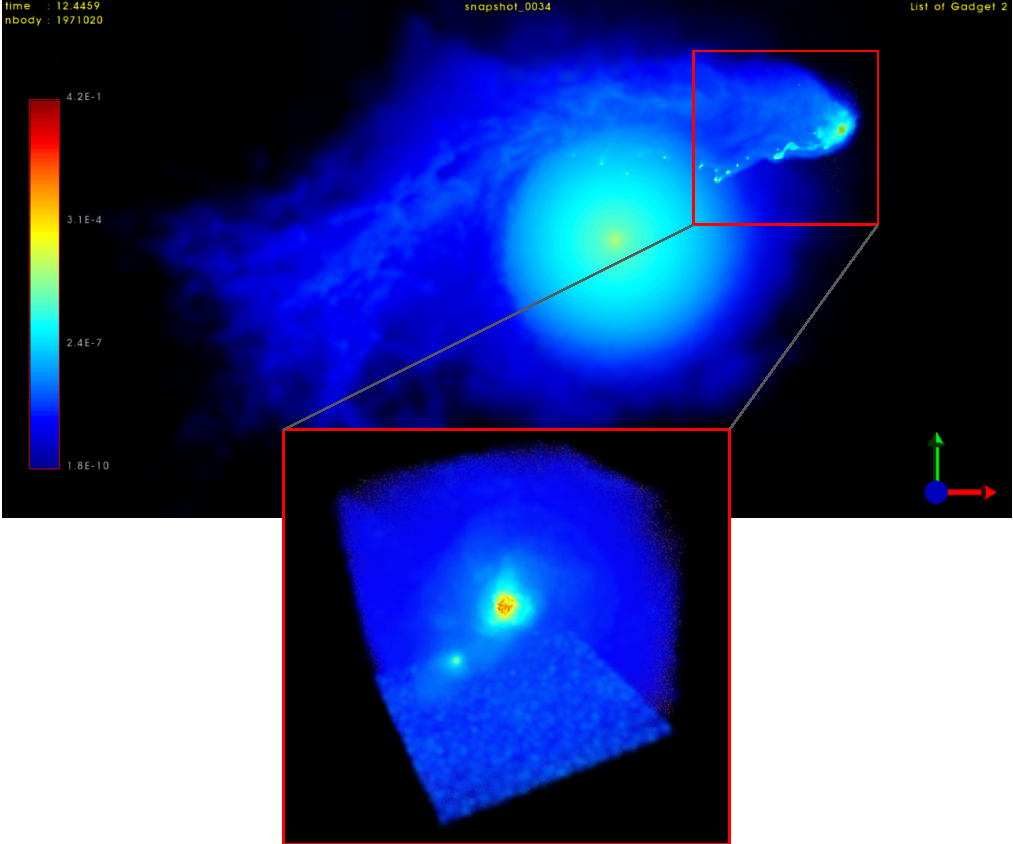
\includegraphics[width=\textwidth]{MovingBox.pdf}
 \caption{An illustration, top panel, of a full fledged simulation of a dwarf galaxy with a Fornax-like cluster.
 Colors show the gas density \citep[using the \texttt{glnemo2} software][]{Lambert2012}.
 Note the number of particles involved, almost 2 millions.
 The moving box technique, represented in the boxy inset, allows to concentrate resources on the interesting part of the simulation.
 Also, at the dwarf-cluster interface an increased resolution is possible, better resolving the stripping.}
 \label{fig:MovingBox}
\end{figure}

We have opted to use the moving-box technique described by \citet{Nichols2015} and further developed by \citet{Hausammann2019}.
As shown in Figure~\ref{fig:MovingBox}, we enclose the MoRIA dwarf in a $60$~kpc wide moving simulation box, as in a wind tunnel simulation.
Gas is injected from the open ``front" side of the box, which always points in the dwarf's direction of motion. Its density and temperature vary with position, as discussed below in Section \ref{sec:fornax_sim}.
This mimics the hot wind of the cluster halo gas as it streams past the orbiting dwarf galaxy.
Also, additional fictitious forces on the particles are included to take into account the rotation and orbital motion of the moving box.
This allows us to simulate the combined effects of tidal forces and ram-pressure stripping \citep[as studied by][]{Mayer2006} which are acting simultaneously on the dwarf without the necessity of simulating a galaxy cluster worth of intra-cluster gas.
% A typical simulation snapshot contains around $150$k gas particles and $16$k star particles, each with a mass of $4000$~\Msun{}.

\subsection{Quaternions}
For completeness, we briefly introduce quaternion algebra \citep{Hamilton1866}.
Following \citet{Graf2008}, a quaternion is a set of four parameters, a real value $q_0$ and three imaginary values $q_1\vect{i},q_2\vect{j},q_3\vect{k}$ with $q_1,q_2,q_3 \in \mathbb{R}$ usually represented as:
\begin{equation}
 \quat{q} = q_0 + q_1\vect{i} + q_2\vect{j} + q_3\vect{k}.
\end{equation}

The core of quaternion algebra is Hamilton's rule for multiplication of the imaginary units $\vect i, \vect j, \vect k$:
\begin{equation}
 \vect i^2 = \vect j^2 = \vect k^2 = \vect{ijk} = −1,
 \label{eq:hamilton_quaternion}
\end{equation}
from which a complete set of non commutative multiplication rules can be derived.
In fact, noting for example that by left multiplying the last equality in eq. \eqref{eq:hamilton_quaternion} by $\vect i$: $\vect i\,\vect{ijk}=-\vect{jk} = -\vect i$, the product of the imaginary parts are:
\begin{equation}
 \vect{ij} = \vect k, \, \vect{jk} = \vect i, \, \vect{ki} = \vect j.
 \label{eq:hamilton_quaternion_mixed}
\end{equation}

Another useful representation of a quaternion is as a pair $\quat{q} = (q_0, \vec q)$ of a scalar part $q_0\in \mathbb{R}$ and a vector part $\vec q \in \mathbb{R}^3$ (also called real and imaginary parts, respectively).
\footnote{Only in this section, to distinguish between quaternions and three dimensional-space vectors, we'll use boldface $\quat{q}$ for quaternions and $\vec q$ for $\mathbb{R}^3$ vectors. In the other sections the difference among the two will be clear from the context.}
Its conjugate~$\conj{\quat{q}}$ is defined as:
\begin{equation}
 \conj{\quat{q}} = (q_0, -\vec q),
 \label{eq:conjugate}
\end{equation}
and its norm as:
\begin{equation}
 \norm{\quat{q}} = \sqrt{q_0^2+q_1^2+q_2^2+q_3^2}.
\end{equation}

From eqs. \eqref{eq:hamilton_quaternion} and \eqref{eq:hamilton_quaternion_mixed} in particular we can write the general formula for the non commutative quaternion multiplication, i.e. given two quaternions $\quat{q}$ and $\quat{p}$:
\begin{equation}
 \quat{q} \,\quat{p} = (q_0 p_0 - \vec q \vdot \vec p, \, q_0 \vec p + p_0 \vec q + \vec q \cross \vec p).
 \label{eq:quaternion_multiplication}
\end{equation}
From \eqref{eq:conjugate} it follows that $\quat{q} \,\conj{\quat{q}} = \norm{\quat{q}}^2 \equiv (\norm{\quat{q}}^2, \vec 0)$. For unit quaternions ($\norm{\quat{q}} = 1$), we can write $\conj{\quat{q}} = \quat{q}^{-1}$.% because $\vect 1 \equiv (0$.

\paragraph{Quaternions and rotations} Unit quaternions are also called \emph{rotation quaternions}.
They can be used to completely describe a rotation of an angle $\varphi$ around the axis $\vec q$.

Let's consider a unit quaternion $\quat{q}$. It can be always written as:
\begin{equation}
  \label{eq:quaternion_with_angle}
 \quat{q} = (q_0, \vec q) = (\cos \frac \varphi 2, \sin \frac \varphi 2\, \hat n), \quad \text{with } \norm{\hat n}=1,
\end{equation}
where $\hat n \equiv \vec q/\norm{\vec q}$ is the versor of $\vec q$.\\
A vector in three-dimensional space $\vec x \in \mathbb R^3$ can be expressed as a \emph{pure quaternion}, a quaternion with no real part: $\vect x = (0, \vec x)$.
% It can therefore multiplied by a quaternion using relation \eqref{eq:quaternion_multiplication}.

The vector $\vec x'$ resulting from the rotation of $\vec x$ of an angle $\varphi$ around the axis $\vec q$ is given by the conjugation operation:
\begin{equation}
\vect x' = \conj{\quat{q}}\, \vect x \, \quat{q}
\end{equation}
where $\vect x' = (0, \vec x')$ \citep[for a proof, see e.g.][sec. 1.4]{Graf2008}.

It is interesting to note that given two unit vectors $\hat{v}_1, \hat{v}_2$, the inverse operation of finding a quaternion $\quat{q}$ which rotate $\hat{v}_1$ into $\hat{v}_2$ can be found as:
\begin{equation}
  \label{eq:quaternion_from_two_versors}
  \quat{q} = \frac{\quat{q^*}}{\norm{\quat{q^*}}}   \qquad \text{with }
  \quat{q^*} = (\hat{v}_1 \vdot \hat{v}_2 + 1, \hat{v}_1 \cross \hat{v}_2).
\end{equation}
In fact, $\hat{v}_1 \vdot \hat{v}_2 = \cos{\varphi}$ (with $\varphi$ the angle between  $\hat{v}_1$ and $\hat{v}_2$) is double the angle of the rotation required by equation \eqref{eq:quaternion_with_angle}.
To get the correct rotation we summed the ``no rotation" quaternion $(1, \vec 0)$ to it and normalized the result.
In the special case that $\hat{v}_1 = -\hat{v}_2$, the resulting quaternion is $(0, \hat{v}_1^\perp)$ with $\hat{v}_1^\perp$ any unit vector perpendicular to $\hat{v}_1$ (\ie{} a rotation of $\pi$ around any orthogonal vector).

In the following sections we'll write equations that involve the rotation a quaternion by a vector.
With a slight abuse of notation we will write directly $\vect x' = \conj{\quat{q}}\, \vect x \, \quat{q}$, considering that the vector indicated in boldface $\vect x$ should be understood to be the pure quaternion $(0, \vec x)$.% given that it will be clear from the context what is a quaternion (mainly just $\quat{q}$).



\subsection{Velocity and acceleration of the particles in the moving box}
\paragraph{Reference frames}
\begin{figure}[H]
 \centering
 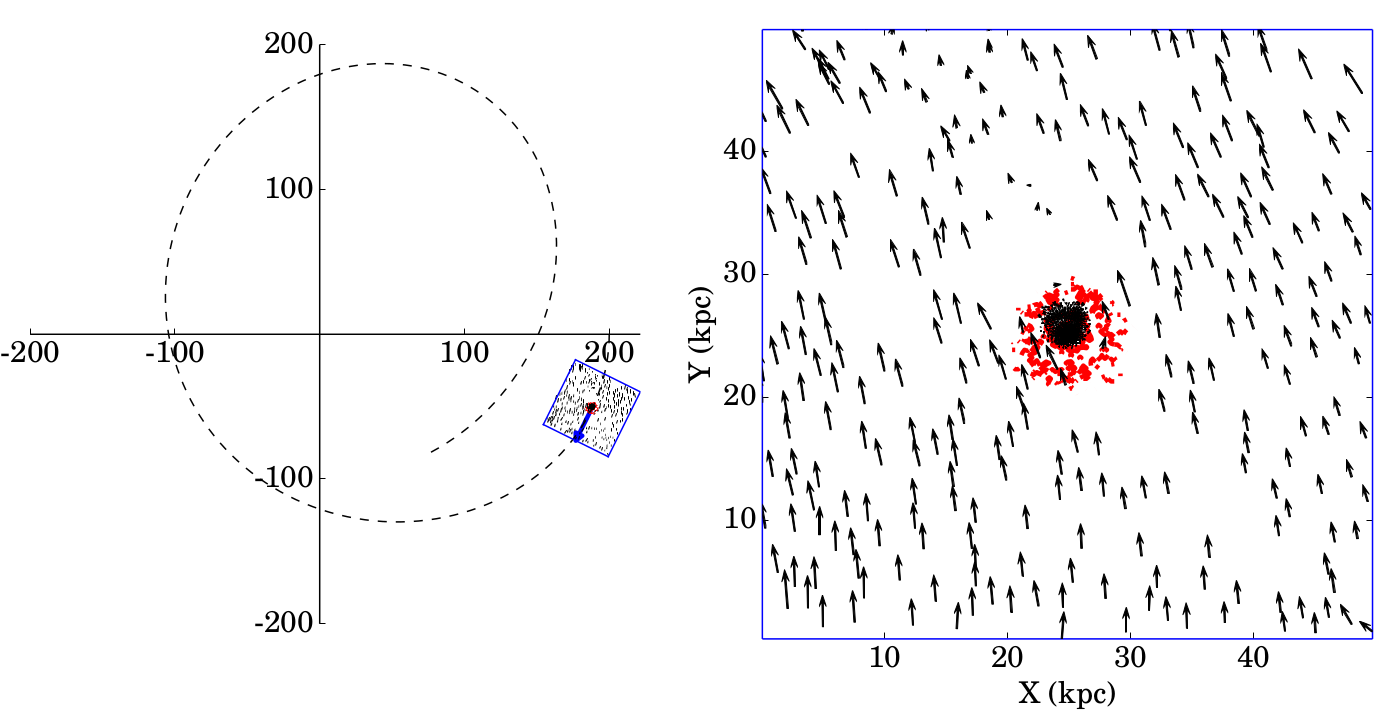
\includegraphics[width=\textwidth]{moving_box_nichols.png}
 \caption{From \citet{Nichols2015}. On the left it is shown the the moving box trajectory. The blue arrow represents the instantaneous box (and therefore dwarf galaxy) velocity.
 On the right, gaseous particles are injected from the bottom side of the box. In red, dark matter density contours, and arrows indicate the wind particles velocity.}
 \label{fig:mb_nichols}
\end{figure}
In a moving box simulation we define the inertial reference frame where the cluster is at the origin.
Relative to that, the box moves and rotates, as shown in Figure \ref{fig:mb_nichols}.
Following the convention in \citet{Nichols2015}, capital letters are used for vectors in the inertial frame whereas small letters for vectors in the moving box (rotating frame).

Let $\quat{q}$ be the quaternion which at each point in time maps the~$-y$ axis of the rotating reference frame to the direction of the velocity of the box in the inertial frame, $\Vp$.
Therefore, a vector $\vect X$ in the inertial frame, corresponds to $\vect x = \conj{\quat{q}}\, \vect X \,\quat{q} $ in the rotating frame.
% To represent the correct rotations, at each moment the quaternion  the moving box is computed.
A fixed point inside the moving box is taken as a reference point, the so called \emph{pivot}, whose coordinates relative to the box are $\xp$ and its velocity and acceleration in the inertial frame relative to the cluster are denoted with $\Vp$ and $\Ap$, respectively.
The \emph{pivot} represents the position in the box of minimum specific energy (the average position of the 64 particles with minimum total potential and kinetic energy) at the start of the simulation and is used to track the velocity and the acceleration of the box.

For a generic particle, the velocity in the moving box reference frame is:
\begin{equation}
 \label{eq:mb_velocity}
 \vect{v} = \quat{q} \,\Vp\, \conj{\quat{q}} - \vect \omega\cross(\vect x -\xp),
\end{equation}
and its acceleration:
\begin{equation}
 \label{eq:mb_acceleration}
 \vect{a} = \quat{q} \,\Ap\, \conj{\quat{q}} - 2\,\vect \omega \cross \vect{v} - \vect\omega \cross ( \vect \omega \cross (\vect x-\xp)) - \dot{\vect \omega}\cross(\vect x -\xp).
\end{equation}


\subsection{Critically damped oscillator}
The acceleration of the pivot point is due mainly to the gravitational attraction of the cluster.
The dwarf galaxy experiences also a low intensity drag due to the gas impinging the galaxy.
%In our simulations, this drag is always $<5\%$ than the gravitational acceleration.
In order to keep the galaxy at the center of the box, an \emph{ad~hoc} corrective acceleration $\Ap^{hoc}$ is added to it as it moves.
This translates to adding an acceleration term to the pivot $\Ap = −\grad \Phi(\vect X_\mathrm p) + \Ap^{hoc}$.

In \citet{Nichols2015}, the correction term is intended to become zero when not needed.
In practice, the $64$ particles with lower total energy (kinetic plus potential) are tracked at each timestep and their average position ($\vect X_{64}$) is taken as the center of the galaxy.
The goal of the ad hoc acceleration is to move the box to follow the center of the galaxy and so compensate the drift of these particles from the pivot.
In the original implementation, $\Ap^{hoc}$ is put to zero as soon as the velocity of the central low energy particles is again directed towards the pivot point (i.e. $(\vect X_{64}-\vect X_\mathrm p) \vdot (\vect{V}_{64} - \Vp) < 0$).
This understandably is done to minimize the total impulse due to the ad hoc term.
But this sudden acceleration removal can cause active particles during the numerical time integration to be kicked away unnaturally, because of the particle acceleration in equation \eqref{eq:mb_acceleration}.
An improvement in our implementation of the moving-box method is the use of a critically damped oscillator for the \emph{ad~hoc} acceleration.
\begin{equation}
 \Ap^{hoc} = 2\,\zeta\omega_0 \Vp + \omega_0^2 \vect X_\mathrm p,
\end{equation}
where $\omega_0$ is the undamped angular frequency of the oscillator, and $\zeta$ the damping ratio.

We start by noting empirically that for our typical galaxy size a sufficient acceleration requires that $\omega_n^2\approx 10$ Gyr$^{-2}$.
Given that we want to dump the oscillation as fast as possible. We use a critically damped oscillator  for which $\zeta = 1$. Therefore the viscous coefficient $2\,\zeta\omega_0$ is simply $6.3$~Gyr$^{-1}$.
A typical behaviour of the \emph{ad~hoc} acceleration is shown in Figure \ref{fig:adhoc}.

\begin{figure}
\centering
  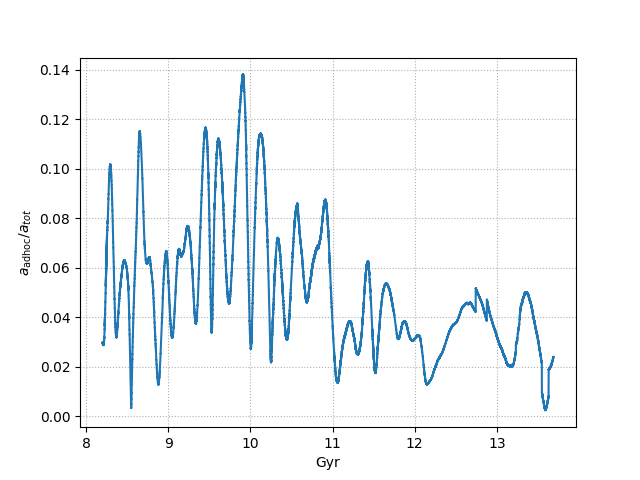
\includegraphics[width=0.8\textwidth]{adhoc69p200i.png}
\caption{Adhoc acceleration relative to the total gravitational acceleration of the simulation ID 69 with pericenter 200 kpc.}
\label{fig:adhoc}
\end{figure}


\subsection{Recovering the correct kinematics from a moving box simulation}
\label{sec:correct_kinematics}
We are interested in finding the expression of the velocity $\vect{V}$ in the inertial frame at a certain position $\vect{x}$ in the moving box, knowing its velocity in the rotating frame $\vect{v}$.
Let $\vect{\Omega}$ be the angular velocity of the box in the inertial frame which can be computed as:
\begin{equation}
 \vect{\Omega} = {(\Vp\cross\Ap)}/{\Vp^2}.
\end{equation}
In the rotating frame the angular velocity of the box can be expressed as:
\begin{equation}
\vect \omega = \conj{\quat{q}}\, \vect{\Omega}\, \quat{q}.
\end{equation}
We can then transform back from rotating to inertial coordinates by applying this transformation:
\begin{equation}
\vect{V} = \Vp + \quat{q} \, \left(\vect{v} + \vect{\omega} \cross (\vect{x}-\xp)\right) \,\conj{\quat{q}}
\end{equation}
where $\mathbf x$ and $\mathbf v$ are position and velocity of the particle in the rotating frame, respectively, and $\mathbf V$ its velocity in the inertial frame. % For simplicity in the following we don't take into account $\Vp$ since its contribution to the line of sight velocity is negligible.

\subsection{Injecting and removing particles in the moving box}
The wind of the moving box is due to particles belonging to the cluster injected with correct velocity, density and temperature in the box.
We assume the cluster gas to have the density and pressure of the Fornax cluster as described by \citet{Paolillo2002} and in \refsec{sec:ICM}. We also assumed zero metallicity and $\alpha-$abundance.

The cluster gas is injected using a sort of ``cartridge'' of particles previously computed as a unit sized cubic glass structure of $N_{\text{glass}} \approx 18000$ particles.
The glass is generated from a random distribution of particles letting them evolve in a periodic box with negative gravitational attraction (effectively being a repulsive force).
The resulting low energy distribution of particles guarantees a low probability of injecting dense clumps of particles which would have high kinetic energy once released.

At each timestep the correct amount of new particles to be injected is taken from the ``cartridge''.
The number of particles belonging to the cluster $N_c$ would be the correct amount to fill up the entire box of size $L$ with the correct cluster density $\rho_c(r)$ at the instantaneous orbital radius $r$.
Therefore they respect the relation:
\begin{equation}
 N_c m_g = \rho_c(r) L^3.
\end{equation}

The fraction of particles to be taken from the cartridge is then: $\xi=\dfrac{N_c}{N_{\text{glass}}}$. The number of particles in the glass should be chosen in order for $\xi\leq1$.
A slice of the glass unit cube is then taken in such a way that its depth is
\begin{equation}
\frac{\norm{\Vp}\Delta t}{L} \sqrt[3]{\xi},
\end{equation}
and width and length are both $\sqrt[3]{\xi}$. The density and the temperature of the new particles are set according to the quantities instantaneous radial distance of the galaxy, the pressure and energy computed using the equation of state.
By construction the new particles have velocity $\norm{\Vp}$ directed towards the local moving box axes $+y$.

If a particle of any kind gets closer than $L/100$ from the rear edge of the box, it gets deleted.
The lateral edges of the box are periodic for gas particles, to keep a constant flow around the galaxy, but dark matter or stellar particles are removed if closer than $L/500$ from any lateral edge of the box.
This process has been fine tuned and extensively tested by \citet{Nichols2015} and \citet{Hausammann2019}.

% It's worthwhile noting that the implementation the deletion or creation of particles in distributed code as the \textsc{Gadget-2} is not a trivial task.
% The arrays representing the particles undergo this kind of algorithm.
% In the end, a rolling

\section{Simulating the Fornax cluster environment}
\label{sec:fornax_sim}

\subsection{Cluster model}

\subsubsection{Dark matter}
The simulations take into account both ram pressure stripping and the tidal interaction with the cluster.
The latter is simulated as a single spherically symmetric static NFW potential profile \citep{Navarro1996} with mass $M~=~10^{14}$~\Msun{} \citep{Drinkwater2001a}:
\begin{equation}
    \Phi(r) = \frac{G M}{r} \frac{\log(1+r/R_s)}{\log(1 + c) - \frac{c}{1+c}}
\end{equation}
with scale length $R_s = 120$ kpc and $c=8.15$ derived from scaling relations in e.g. \citet{Gentile2004, Wechsler2002}:
\begin{equation}
    c \simeq 20 \left(\frac{M}{10^{11} \text{\Msun{}} }\right)^{-0.13}, \qquad
    R_s = \frac 1 c \left(\frac{M}{\frac 4 3 \pi 200 \rho_c}\right)^\frac 1 3,
\end{equation}
with $\rho_c = 127.3$~\Msun{}~kpc$^{-3}$ the critical density of the universe at $z=0$ for a cosmology with Hubble constant $h=0.67$ and $\Omega_m = 0.31$ \citep{Planck2015}.
The cluster virial radius of the model is $R_{\mathrm{vir}} = c R_s = 978$~kpc.

\subsubsection{ICM} \label{sec:ICM}
Following \citet{Paolillo2002}, we use the superposition of three spherically symmetric beta-models, $\rho(r) = \rho_0 (1 + (r/r_0)^2 )^{-3\beta/2}$, to construct the gas density profile in the Fornax cluster, as shown in Figure \ref{fig:profiles}.
They identify three contributions to the hot gas distributions: a central component (dominating for $r<5''$), coincident with the optical galaxy NGC1399; a less dense and more extended galactic component ($50''<r<400''$); and a cluster component ($r>400''$).
We assume the gas to be in hydrostatic equilibrium with temperature $T(r)$ computed as:
\begin{equation}
   T(r) = \frac {m_p}{k_B \rho(r)} \int_r^\infty \rho(r') \frac{GM(r')}{r'^2} \dd{r'}
\end{equation}
where $M(r)$ is the mass of the gas, stars and dark matter beyond radius $r$, $m_p$ is the proton mass, $G$ and $k_B$ the gravitational and Boltzmann constants.

\begin{figure}[H]
\centering
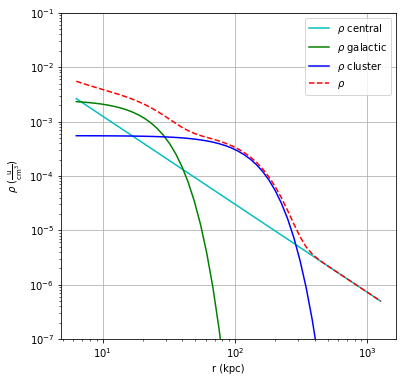
\includegraphics[width=0.65\textwidth]{PaolilloRho.png}
\caption{Gas density profile $\rho(r)$ of the  Fornax Cluster model as a superposition of three beta models from measurements described in \citet{Paolillo2002}, from which we also adopt the nomenclature for the different beta models.
}
\label{fig:profiles}
\end{figure}

These two radial profiles allow us to inject particles with the proper density and temperature in the moving box, hence recreating the environmental condition of the cluster as the dwarf orbits through it.

\subsection{Simulation parameters}
We carried out a set of simulations starting from five MoRIA models of late-type galaxies taken at $z = 0.5$.
The overall goal in setting up the simulations is to study the evolution of late-type galaxies in a cluster environment.
The choice of the redshift of infall has been motivated by the fact that the number of red dwarfs in the Fornax cluster has increased significantly since $z = 0.5$ \citep{Stott2007, DeRijcke2010}.
That indicates that the conversion of late-type to early-type dwarfs (and hence the acquisition of late-type dwarfs by clusters) is probably a recent event.

We selected dwarfs models covering the stellar mass range of $10^{7.5}-10^{9}$ and we injected each of them on 5 different orbits with pericenter distances of $50, 100, 150, 200,$ and $300$~kpc and with a fixed apocenter of 800 kpc.
The starting point of the infall is always at a radial distance of 600~kpc.
We chose a lower radial distance of the starting position with respect to the virial radius given the very low cluster density in that region and the low orbital velocity of the dwarf near apocentre.
In this way, simulations could be concentrated on the infall and the pericenter passages of the simulated dwarfs.
We evolved the galaxies for $5.5$~Gyrs up to $z=0$.
The initial stellar masses are reported in Table \ref{tbl:sim}.
All simulations presented in this paper, at time of injection have exponentially declining SB profiles with Sersic index around 1.0.
Every $10$~Myr a snapshot is saved, yielding around 560 snapshots for each simulation.
This high snapshot cadence has proven to be important for the following analysis (see \refsec{sec:morphological_quest}).
Adhering to the simulation goal of following the evolution of a gas-rich late-type dwarf in a Fornax-like cluster, the initial snapshot of the most massive dwarf (ID 41) has been taken at $z=0.4$ because at $z=0.5$ it was still undergoing a major merger event.
This is equivalent to having this galaxy falling into the cluster more recently.
No sizeable effect has been noted in simulations results highlighting a different behaviour with respect to the other galaxies \citep[which underwent their last merger before infalling to the cluster at $z=0.5$, see e.g.][]{Cloet-Osselaer2014}.
This has had the only implication of a lower number of snapshots used in the technique explained in \refsec{sec:morphological_quest}, but, as we shall see in the following, given that first pericenter passage turns out to be the most significant orbital phase, no notable bias is expected.

\begin{table}
\centering
\footnotesize
\begin{tabular}{cx{1.3cm}x{0.5cm}x{0.8cm}x{0.7cm}x{0.4cm}x{1.4cm}}
\toprule
Sim ID & $\log_{10}$(M$_\star$)\newline(M$_\odot$) & $R_e$ \newline (kpc) & $\sigma_\star$ \newline (km/s)\\
\midrule
  62 &  6.66 &  0.8 &  11.4 \\%&  -11.8 &  0.5 &  25.8 \\
  71 &  7.58 &  1.9 &  21.9 \\
  68 &  7.96 &  2.6 &  15.6 \\
  69 &  8.04 &  2.3 &  24.6 \\
  41 &  8.78 &  1.7 &  30.4 \\
\bottomrule
\end{tabular}
\caption{Features at time of infall ($z=0.5$) of the selected MoRIA dwarf models used in this work}
\label{tbl:sim}
\end{table}


\section{Only tides simulations}
In order to isolate the effects of the tides and of the ram pressure, we performed some representative simulations without the cluster gas.
% These hypothethical simulations show...

In Figure~\ref{fig:gas_no_gas}, are shown the typical tidal tails due to tides...
% TODO

\begin{figure}[ht]
 \centering
%  \includegraphics[width=0.8\textwidth]{gas_no_gas.png}
 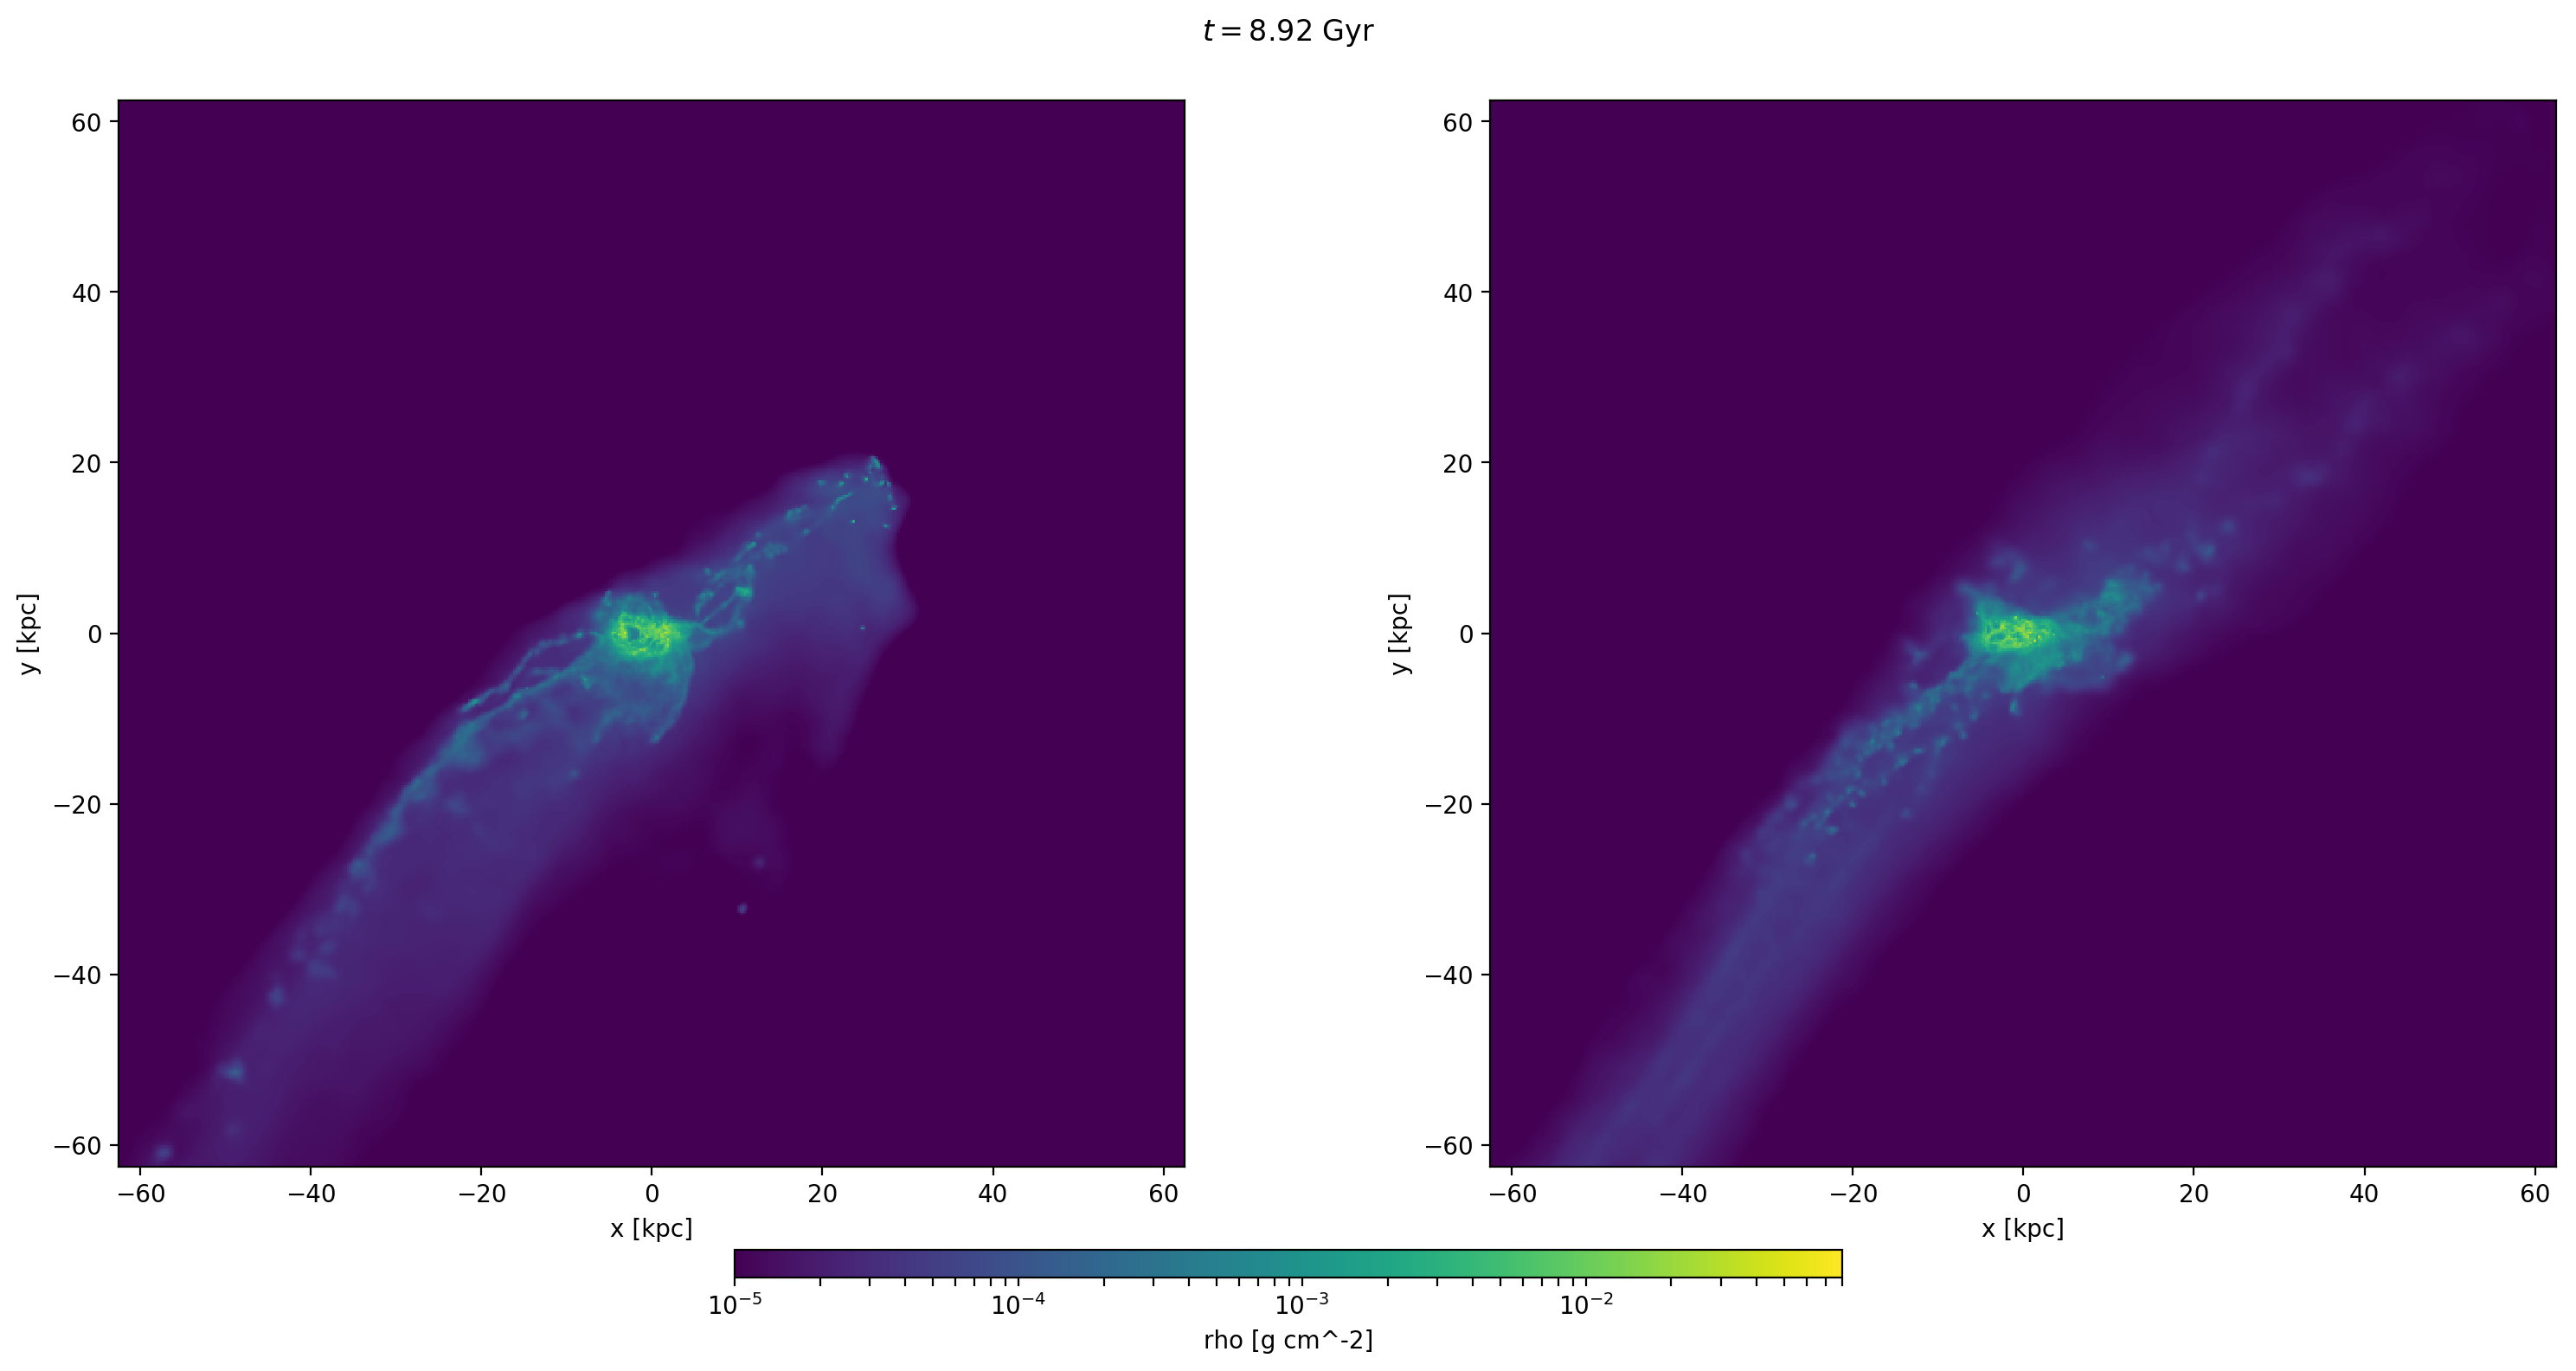
\includegraphics[width=\textwidth]{stripping2.png}
 \caption{Projected gas density map of a galaxy orbiting a Fornax-like cluster.
 On the right, the gas interacting with the dwarf creates a wake and a single tidal tail is formed; on the left a snapshot without cluster gas: two tidal tail are shown.}
 \label{fig:gas_no_gas}
\end{figure}


% !TEX root = thesis.tex

\chapter{Simulation results}
\label{ch:sim_results}

We present here the results of the simulations performed using the technique presented in the previous Chapter.
We will concentrate on following the journey of the galaxy into the cluster and characterize its evolution depending on the initial mass at the time of injection and its orbit.
Generally, galaxies will undergo some ``phase transitions" which will happen mainly at pericenter passages.
Some of the galaxy will effectively be transformed into Ultra Diffuse Galaxies (as shown in Section~\ref{sec:UDG}), some other will be allowed to briefly be identified as ``jellyfish" (Section~\ref{sec:where_star_formation}).

\begin{sidewaystable}
 \centering
 \footnotesize
 \begin{tabular}{lx{0.8cm}x{1.4cm}x{0.7cm}x{1cm}x{0.8cm}x{0.8cm}x{0.7cm}x{1.9cm}}
\toprule
name & peric. \newline (kpc) & $\log_{10}$(M$_\star$) \newline (M$_\odot$) & $R_e$ \newline (kpc) & $\sigma_\star$ \newline (km/s) & M$_V$ \newline (mag) & M$_{r'}$ \newline (mag) & $n$ & $\bar{\mu}_{e,r'}$ \newline (mag/arcsec$^2$) \\
\midrule
  62 &                        50 &                                        6.50 &                  1.6 &                            6.7 &                 -9.7 &                   -10.1 & 1.1 &                                         28.7 \\
  62 &                       100 &                                        6.57 &                  1.6 &                            8.0 &                 -9.9 &                   -10.2 & 1.0 &                                         28.5 \\
  62 &                       150 &                                        6.59 &                  1.6 &                            9.1 &                 -9.9 &                   -10.2 & 1.4 &                                         28.6 \\
  62 &                       200 &                                        6.59 &                  1.7 &                            8.3 &                -10.0 &                   -10.3 & 1.2 &                                         28.5 \\
  62 &                       300 &                                        6.64 &                  1.7 &                            8.6 &                -10.1 &                   -10.4 & 1.0 &                                         28.2 \\
  71 &                        50 &                                        6.26 &                  6.7 &                           21.6 &                 -9.5 &                    -9.8 & 0.0 &                                         31.8 \\
  71 &                       100 &                                        6.82 &                  6.2 &                            6.5 &                -10.9 &                   -11.2 & 0.5 &                                         30.5 \\
  71 &                       150 &                                        6.79 &                  6.4 &                            0.8 &                -10.7 &                   -11.0 & 0.5 &                                         30.5 \\
  71 &                       200 &                                        6.85 &                  6.9 &                            0.8 &                -11.0 &                   -11.3 & 0.2 &                                         30.4 \\
  71 &                       300 &                                        6.85 &                  7.2 &                            1.8 &                -11.0 &                   -11.4 & 0.2 &                                         29.7 \\
  69 &                        50 &                                        6.81 &                  7.6 &                            1.6 &                -10.6 &                   -11.0 & 0.2 &                                         30.7 \\
  69 &                       100 &                                        7.53 &                  7.1 &                           17.8 &                -12.5 &                   -12.9 & 0.1 &                                         28.4 \\
  69 &                       150 &                                        8.05 &                  4.3 &                           11.6 &                -14.2 &                   -14.4 & 0.3 &                                         26.8 \\
  69 &                       200 &                                        8.34 &                  3.3 &                           18.4 &                -15.0 &                   -15.3 & 1.0 &                                         25.0 \\
  69 &                       300 &                                        8.42 &                  1.8 &                           23.9 &                -15.5 &                   -15.7 & 0.9 &                                         23.5 \\
  68 &                        50 &                                        6.27 &                  8.0 &                            nan &                 -9.1 &                    -9.4 & 0.0 &                                         32.3 \\
  68 &                       100 &                                        6.85 &                  7.3 &                            2.5 &                -10.6 &                   -10.9 & 0.1 &                                         31.2 \\
  68 &                       150 &                                        6.85 &                  7.3 &                            nan &                -10.6 &                   -10.9 & 0.1 &                                         31.2 \\
  68 &                       200 &                                        7.02 &                  7.4 &                            nan &                -11.4 &                   -11.7 & 0.1 &                                         30.0 \\
  68 &                       300 &                                        8.09 &                  3.8 &                           11.5 &                -14.5 &                   -14.8 & 0.8 &                                         26.2 \\
  41 &                        50 &                                        8.93 &                  3.5 &                           16.5 &                -16.2 &                   -16.5 & 1.0 &                                         23.9 \\
  41 &                       100 &                                        8.94 &                  2.5 &                           26.0 &                -16.4 &                   -16.7 & 1.0 &                                         23.0 \\
  41 &                       150 &                                        8.99 &                  1.7 &                           28.5 &                -16.6 &                   -16.8 & 0.8 &                                         22.2 \\
  41 &                       200 &                                        8.97 &                  2.2 &                           29.4 &                -16.6 &                   -16.8 & 0.8 &                                         22.5 \\
  41 &                       300 &                                        9.04 &                  1.8 &                           33.7 &                -17.0 &                   -17.2 & 0.7 &                                         21.8 \\
\bottomrule
\end{tabular}

 \caption{Features of the selected MoRIA galaxies at $z=0$.} \label{tbl:galaxies}
\end{sidewaystable}

In Table \ref{tbl:galaxies} we present the final value of some physical values at the end of the simulations which were performed from $8.5$~Gyr to $\approx 14$~Gyr\footnote{We highlight that each simulation required $\approx 25$ days on average of wall clock runtime on dedicated computing nodes with 32 cores.
}.
Before starting the exposition, we have to introduce a couple of concepts which revealed particularly useful in the analysis and allowed for better comparison among the different MoRIA galaxies and the orbits introduced above.

\paragraph*{Radial period}
Pericenter passages, as explained in the following, are important moments for the life of the simulated dwarf.
In order to compare different orbits, we normalise the simulation time by the orbital radial period $T_r$, \ie{} the time between two pericenter passages, \citep[p.~146]{BinneyTremaine2008}:
\begin{equation}
    T_r = 2 \int^{r_a}_{r_p} \frac{\d r}{\sqrt{2\left[E-\Phi(r) \right] - J^2/r^2}}
    \label{eq:radial_period}
\end{equation}
where $r_p, r_a$ are the pericenter and apocenter distance respectively, $E$ and $J$ the orbital energy and angular momentum per unit mass, $\Phi(r)$ the potential at radius $r$ of the NFW halo around which the galaxy is orbiting.

By defining the time of pericenter passage as $t_p: r(t_p) = r_p$, we can introduce the normalized time:
\begin{equation}
  \label{eq:tau}
\tau = \frac{t-t_p}{T_r},
\end{equation}
which is~$0$ or $1$ for first or second pericenters respectively,~and~$0.5$ for apocenter passages.

% We begin with following one galaxy in its journey around the cluster.
In the following we will compare the effects of orbit and initial mass using the set of 25 simulations we have carried out.


\paragraph*{Tidal radius}
As we shall see, the cluster gravitational potential is able to strip material from the galaxy. Some of the simulations, depending on the orbit they are on, will become gravitationally unbound dominated by the cluster potential.
We chose to define the event of becoming unbound using the condition on the tidal radius \cite{King1962}: namely when it becomes smaller than the effective radius.
This criterion tests whether the stellar body of the galaxy would become unbound and dissolved, which is what an observer would consider for the detection of a ``galaxy''.
Physically, also this implies that orbits of the stars in the outskirts of the galaxy are influenced by the cluster potential more than they are by the galactic halo potential.
Tidal radius $r_t$ is computed as follows:
\begin{equation}
r_t = r \sqrt[3]{\frac{M_g}{M_c(r) (3+e)}},
\label{eq:tidal_radius}
\end{equation}
where $e = (r_a - r_p) / (r_a + r_p)$ is the eccentricity of the orbit computed, $r_a$, $r_p$ the apocenter and pericenter radii respectively; $M_c(r)$ is the enclosed cluster mass at radius $r$, and $M_g$ the instantaneous total mass of the galaxy.
As a convention we measure the galaxy mass as the total mass (baryonic and dark matter) within $10$~kpc from the center of the galaxy.

In Figure \ref{fig:tidal_radius} we show an example of $r_t$ evolution along the orbit.
We define a galaxy to become unbound when the condition
\begin{equation}
    R_e > r_t
\label{eq:tidal_radius_condition}
\end{equation}
first occurs.
%Galaxies on a radial orbits will undergo disruption more easily.
\begin{figure}
\centering
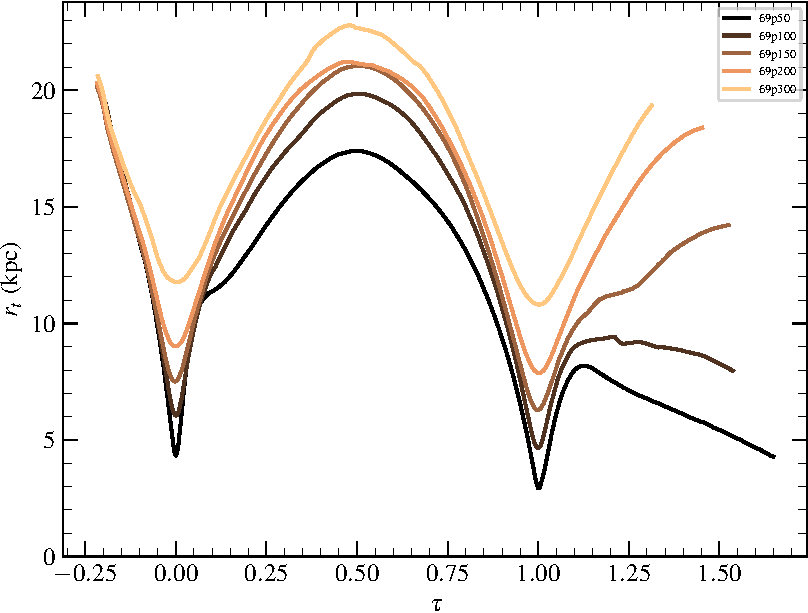
\includegraphics[width=\textwidth]{14.0_tidal_radius.pdf}
\caption{Evolution of the tidal radius for the simulations ID 69.}
\label{fig:tidal_radius}
\end{figure}

\section{Becoming an Ultra Diffuse Galaxy (UDG)}
\label{sec:UDG}

Faint Low Surface Brightness (LSB) galaxies have been detected in galaxy clusters since the 1980s \citep[e.g.][]{Sandage1984}.
% See Wittmann  https://www2.mpia-hd.mpg.de/homes/galClusters_2017/slides/Ringberg2017_presentation_Wittmann.pdf

% Wittmann2017 studies LSB in Perseus
LSB galaxies are defined as having \citep{Venhola2017}:
\begin{equation}
\begin{cases}
 \mu_{0,r'} > 23 \mbox{ mag/arcsec}^2\\
 M_{r'} > -19
\end{cases}
\end{equation}

In 2015 \citet{VanDokkum2015} introduced a size criterion to distinguish between LSB galaxies and more compact `normal' dwarfs \citep{Sales2021}:
UDG are therefore defined as large ($R_e > 1.5$~kpc) low surface brightness galaxies.
%($\bar\mu_{r',e} > 24$~mag/arcsec$^2$).

The majority of studies indicate that they have the properties of large dwarf galaxies \citep{Sandage1984, Roman2017, Venhola2017, Saifollahi2021}.
Three main mechanisms are hypothesized as possible formation scenarios for UDGs:
\begin{itemize}
  \item dwarf galaxies which undergo strong tidal stripping \citep{Venhola2017, Carleton2018, Rong2020a};
  \item gas outflows driven by stellar feedback with extended dark-matter halo and faint and diffuse stellar component \citep{DiCintio2017, ManceraPina2019},
  \item or failed $L_\star$ galaxies\footnote{An $L_\star$ galaxy has a luminosity equal to the characteristic luminosity of the Schechter luminosity function \citep{Press1974}.
  Its value is about $L_\star \approx 3\times10^{11}L_\odot$, \cf{}  \citet{Cooray2005}.}
in high mass dark halos with ceased star formation in the early universe.
\end{itemize}
Some UDGs have earlier been identified as disrupted early-type galaxies.
\citet{Koch2012} is indeed able to reproduce a typical S-shape tidal tailed UDG HCC-087 in the Hydra I cluster via simulations considering only the cluster potential.
It is worth noting that in their simulations they find an orientation of the tidal tails perpendicular to the orbit, which will be important in Chapter~\ref{ch:ngc1427a}.

The cluster alignment of UDGs is also a quantity which in various cluster has been measured.
The signs of elongation, which will be discussed further in~Section \ref{sec:3d_ellipticity}, have been used to infer the origin of UDGs.
In the Coma and Abell 1314 clusters \citep{Yagi2016, ManceraPina2019} UDGs are preferably aligned towards the cluster center.
This suggesting that they may be the products of strong tidal interaction with the cluster.
In the Fornax cluster, however, the low statistics do not allow for a conclusive analysis.
On the other hand at least two of the detected UDGs in Fornax show sign of elongation towards a nearby dwarf galaxy \citep[with $M_{r'} > -19$~mag, see][]{Venhola2017}.
As shown by \citet{Rong2020}, for the Abell 2634 cluster, the minor axes of UDGs tend to be aligned with the major axis of the central dominant galaxy.
It is implied therefore that, in this case, UDGs are possibly very recent infallers, still retaining signs of their primordial alignment in the closest large-scale filament they came from.

\paragraph{UDGs in Fornax}
\citet{Venhola2017} found nine UDGs candidates within an area of $4$~deg$^2$ centered in NGC1399.
The ratio of UDGs to dwarf galaxies in Fornax is consistent with that in the Coma and Virgo clusters.
Also, the number of UDGs within the virial radius are correlated with the virial mass of the cluster.
In the size-magnitude parameter space, UDGs in Coma form a continuous distribution, whereas in Fornax two of them are  remarkably luminous, and can be considered as outliers.
Also, UDGs in Fornax are among the more luminous galaxies and their colour correlates with surface brightness, becoming redder with increasing surface brightness.
They follow the same color-magnitude relation as dwarfs, which suggests a link between UDGs and dwarf galaxies  (\cf{} Section~\ref{sec:CM}).
% As expected, Sérsic index is around $1$
As opposed to the ones in the Coma cluster, their alignment with respect to the cluster potential is not evident: in Coma UDGs are oriented towards the cluster center, whereas in Fornax, as mentioned above, there's no correlation.
It is interesting to note that larger UDGs are more elongated as opposed to UDGs in Coma.

\subsection{Size and magnitudes}
Once approaching the pericenter, energy is transferred to the galaxy, according to the virial theorem.
%According to the virial theorem %predicts that by adding energy to a galaxy, it will increase its radius:
%once approaching the pericenter, energy is transferred to the galaxy:
Stars thus migrate to more energetic and hence wider orbits.
In addition, mass is lost due to tides, making the gravitational well even more shallow and leading to potentially large increases in radius.
We compute the 3D effective radius shown in Figure~\ref{fig:r_eff}.
This radius is independent of the orientation of the galaxy, and it has been computed as the radius of the sphere which contains half the total luminosity of the galaxy.
Tidal heating affects the size of the galaxies as they pass near the cluster center, with low mass galaxies affected most.

% We compare the resulting effective radius in simulations with the ones not taking into account the gas inside the cluster, Figure~\ref{fig:r_eff_no_gas}.

\begin{figure}[ht]
\centering
\includegraphics[width=\textwidth]{{00.0_fig_3dreff_time}.pdf}
\caption{3d effective radius evolution with time normalised with the radial period of the orbit. Curves are smoothed using a rolling average of 0.2~Gyr and are truncated as soon as condition \eqref{eq:tidal_radius_condition} is verified.}
\label{fig:r_eff}
\end{figure}

% NOTE See whether to put this plot
% \begin{figure}
% \centering
% \includegraphics[width=\columnwidth]{{00.2_3dreff_gas_no_gas_last_Re_color}.pdf}
% \caption{Relative change in effective radius between simulations with tides only ($R^{3D}_{e, ng}$), and cluster infall simulations with RPS ($R^{3D}_e$) at redshift $z=0$.}
% \label{fig:r_eff_no_gas}
% \end{figure}
% \subsection{Dark halo concentration}
% Between two pericenters material falls back in the galaxy, see Figure~\ref{fig:dm_halo}.

% NOTE maybe it is better to compare a sphere of 2 kpc with one of 10 kpc, and not comparing spheres with cubes.

% \begin{figure}
% \centering
% \includegraphics[width=0.9\columnwidth]{{12.0_dm_ratio}.pdf}
% \caption{Ratio between dark-matter mass contained in a sphere of $10$ kpc radius $M_h^{c}$ and the total dark-matter mass contained in the moving box, $M_h^{tot}$.}
% \label{fig:dm_halo}
% \end{figure}

% \subsection{Stellar metallicity gradients}

\subsection{$M_h/M_\star$}
We computed the stellar and dark-matter mass inside a sphere of radius $10$~kpc centered on the dwarf and the masses inside the entire moving box.
While stars gets formed around pericenter passages, dark matter instead is pulled out by tidal forces who elongate the halo, effectively stripping dark-matter particles out of the moving box of our simulation setup.
This is confirmed for example by comparing the amount of dark matter inside the $10$~kpc region around the dwarf with the whole dark matter present inside the moving box.
As shown in Figure \ref{fig:dm_center_inflow}, there is an inflow of dark matter towards the dwarf galaxy due to tidal squeezing and compression, soon followed by an expansion, resulting in a dearth of dark matter after the first pericenter passage. % NOTE possibly do dark matter profile around pericenter?
For very radial orbits, around first infall, central halo mass increases more than the stellar mass created by the starburst, Figure~\ref{fig:m_halo_m_star}.

\begin{figure}
\centering
\includegraphics{{12.5_dm_ratio_one_sim}.pdf}
\caption{Relative amount of central dark matter $M_{h}^c$
(computed as the mass inside a sphere of 10~kpc of radius around the galaxy)
with respect to the dark matter in the simulation box ($M_{h}^{tot}$) for sim ID 69.
Colours indicate the pericenter distances of the different orbits.
}
\label{fig:dm_center_inflow}
\end{figure}
\begin{figure}
\centering
\includegraphics[height=0.95\textheight]{{12.1_m_halo_m_star}.pdf}
% \includegraphics[width=0.75\columnwidth]{{12.1_m_halo_m_star}.pdf}
\caption{$M_h/M_\star$ around first infall. Halo and stellar mass are computed in a $10$~kpc sphere around the galaxy.
The different orbits with the respective pericenters are color coded as shown in the legend.}
\label{fig:m_halo_m_star}
\end{figure}

\subsection{Central stellar velocity dispersion}
We measured the central (within $250$ pc) stellar velocity dispersion for all the simulations on their orbits, as shown in Figure~\ref{fig:sigma}.
\begin{figure}[ht]
\centering
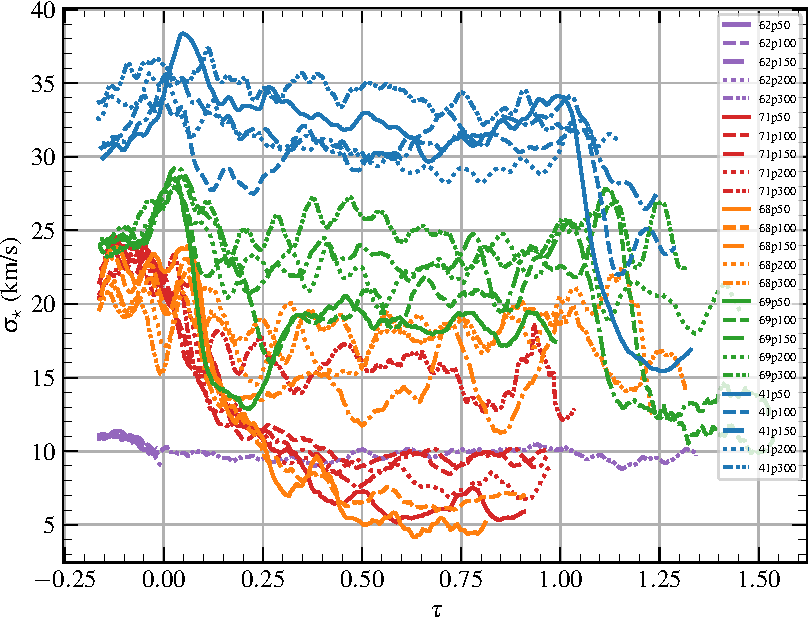
\includegraphics[width=\textwidth]{01.0_fig_sigma_time.pdf}
\caption{The evolution as a function of time (normalized with orbital radial period) of the
line-of-sight velocity dispersion of star particles within a $250$~pc from the galactic center.
Curves are smoothed using a rolling average of 0.2~Gyr.
}
\label{fig:sigma}
\end{figure}
For simplicity we adopted a common point of view for all the orbits, and the line-of-sight velocity dispersion is computed assuming the observer laying in the orbital plane.
As tidal interactions stir the particles in the center of the galaxies, at the pericenter passages a bump in the central velocity dispersion (denoted by~$\sigma$) can be seen.
The following temporary decrease in central velocity dispersion can be linked to the variations of~$M_h/M_\star$.
Tidal squeezing increase~$\sigma$ while subsequent mass loss can dramatically lower it.

\begin{figure}[ht]
\centering
%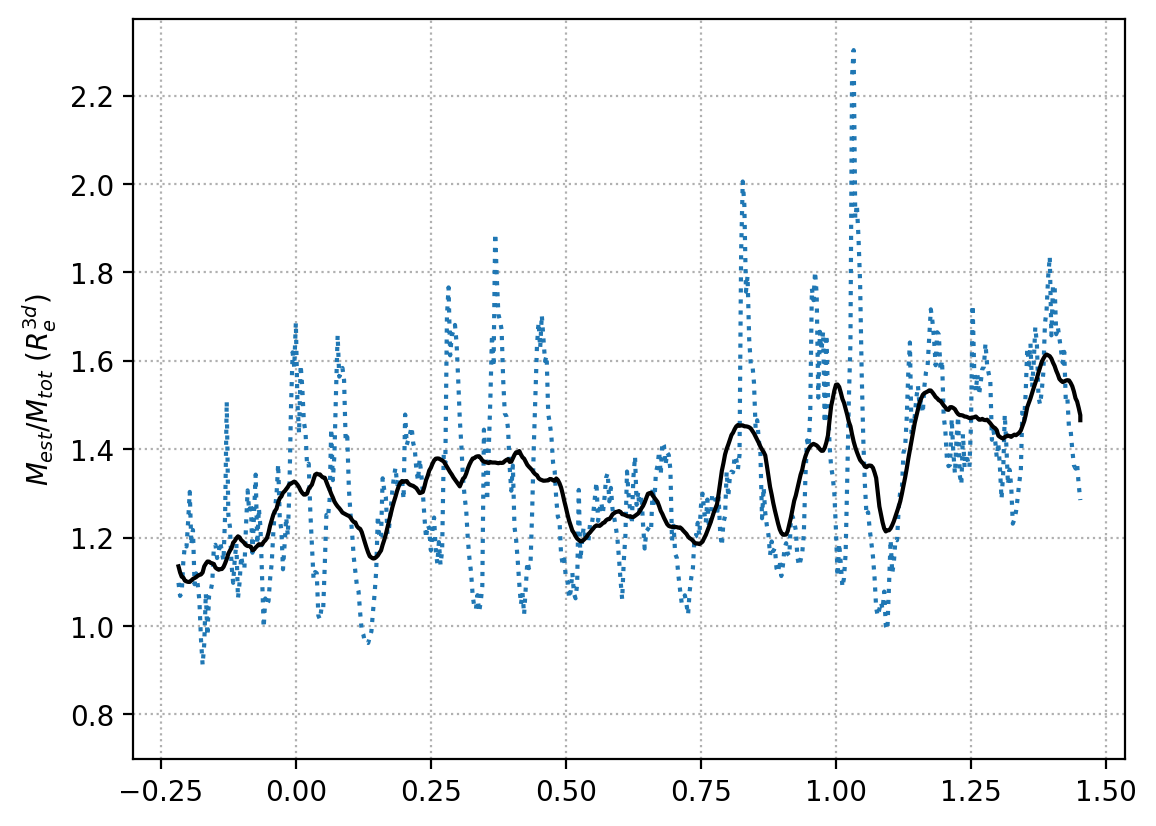
\includegraphics[width=\textwidth]{wolf_m_est_ratio69p200.png}
%\caption{In blue the estimated mass from velocity dispersion with equation \eqref{eq:wolf} relative to the total mass within an effective radius computed from simulation particles,
%for simulation ID 69 on an orbit with 200~kpc pericenter.
%In black the local rolling average with a window of 30 snapshots.
%}
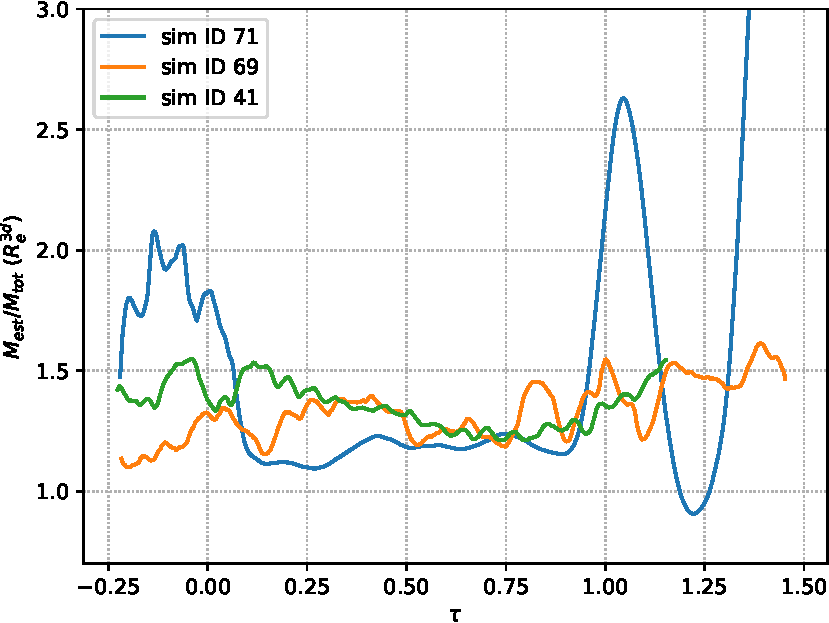
\includegraphics[width=\textwidth]{mass_sigma_multi_sim.pdf}
\caption{The estimated mass from velocity dispersion with equation \eqref{eq:wolf} relative to the total mass within an effective radius computed from simulation particles,
for simulation ID 69, 71, 41 on an orbit with 200~kpc pericenter.
Dashed line is for unbound snapshots (the condition \eqref{eq:tidal_radius_condition} is not verified anymore).
}
\label{fig:wolf}
\end{figure}

We checked the dynamical mass estimation which can be computed from the velocity dispersion using the \citet{Wolf2010} relation:
\begin{equation}
\label{eq:wolf}
M^{dyn}_{est} = \dfrac{3}{G} \sigma_e^2 R_e,
\end{equation}
where $\sigma_e$ is the luminosity-weighted line-of-sight velocity dispersion within an effective radius~$R_e$,
and $G$ the gravitational constant.
The result three representative simulations is shown in Figure~\ref{fig:wolf}.
For the low mass galaxy (simulation ID 71), the estimation is not reliable anymore as soon as the galaxy becomes unbound (dashed line in Figure~\ref{fig:wolf}), \ie{} the condition \eqref{eq:tidal_radius_condition} does not hold anymore.
The method of equation \eqref{eq:wolf} overestimates the mass by $\approx20-50\%$ depending on the orbital phase.
Given the simplicity of the method, this relation between the estimated value and the ground truth mass is quite remarkable.
From this, we can learn that despite some conditions required for the application of the method ---~such as equilibrium and sphericity~--- not being fulfilled, the dark-matter content estimates with this method are reliable within an acceptable relative range.

% NOTE The anisotropy parameter $\beta$ can be taken into account

% \citep{Danieli2019} Low dark matter galaxies.

\subsection{3D ellipticity} \label{sec:3d_ellipticity}
We computed the 3D ellipticity of the stellar component of the galaxies using the Principal Components Analysis \citep[PCA, ][]{Pearson1901}.
The first principal component $\vect{w}_2$ is the direction of highest elongation (largest variance of the star particle positions) computed via PCA\footnote{
$\vect{w}_2$ is defined as the eigenvector corresponding to the largest eigenvalue of the covariance matrix $C = \frac 1 {(N-1)} AA^T$, where $A$ is the matrix of the position of the star particles centered on the barycenter of the stars, and $N$ the number of particles.}.

Around pericenter the main elongation direction of the ellipsoid ($\vect w_2$) is aligned with the cluster center; then it undergoes a ``slingshot effect" after pericenter and it aligns with the cluster center also around apocenter before falling back in. This behaviour is shown in Figure~\ref{fig:pca}.
Around the second pericenter passage, for radial orbits, the galaxy ends up being dispersed and not anymore gravitationally bound.

In Figure~\ref{fig:pca_angle_r}, we show quantitatively the relative orientation between $\vect{w}_2$ and the clustercentric direction for simulation ID 69.
Around both pericenter passages the galaxy becomes aligned with the cluster center.
The maximum alignment is obtained at a delayed time depending on the radiality of the orbit.
Also, for all the orbits, the galaxy shows an aligment of an angle $<30$~deg if the orbital phase lays within a quarter of the radial period soon after pericenter, \ie{} $\tau \in [0, 0.25] \cup{} [1, 1.25]$.
% This translates in a time interval of , , depending on the orbit.
Except for the orbit with 100~kpc pericenter, it is possible to see how at apocenter the main elongation is perpendicular to the cluster center. % For this orbit it is likely that due to a swap between

Analogously, we can compute the angle between the elongation direction and the instantaneous velocity along the orbit.
As shown in Figure~\ref{fig:pca_angle_v}, because of the high relative speed and the delay in the formation of tidal tails, around pericenter passages the angle beteen $\vect{w}_2$ varies significantly.
Interestingly, just before the pericenters, velocity is almost perpendicular to the direction of elongation.
At the same time, stripping intensity is at its peak (see Figure~\ref{fig:r_rps}) creating a gaseous tail aligned with the instantaneous velocity of the galaxy.
This misalignement between the tails is shown in detail in Chapter~\ref{ch:ngc1427a} and can be used to infer orbital properties of observed galaxies in cluster.

\begin{figure}
\centering
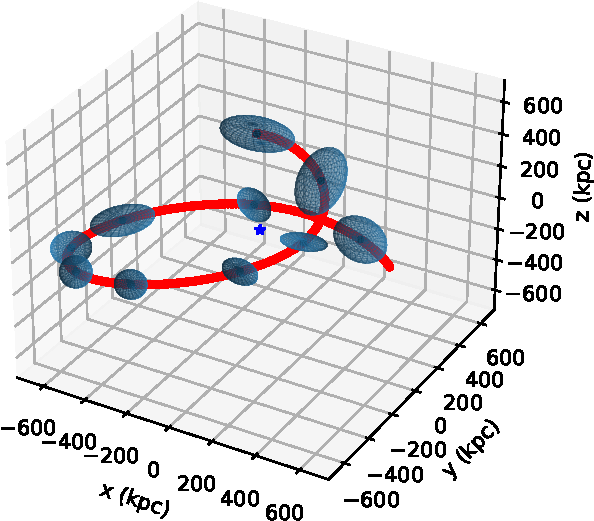
\includegraphics[width=\textwidth]{3d_qualitative_69p200.pdf}
\caption{Qualitative overview of the principal components ellipsoids for the stellar particle positions of the galaxy along its orbit.
In red the orbit of the galaxy, ID 69 with pericenter of 200 kpc.}
\label{fig:pca}
\end{figure}

\begin{figure}
\centering
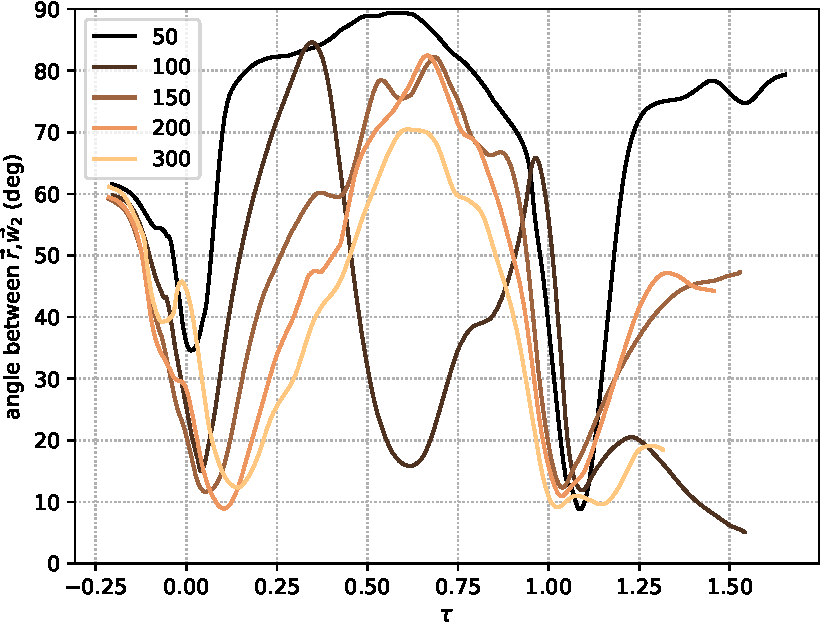
\includegraphics[width=0.8\textwidth]{69_r_angle.pdf}
\caption{Angle between the largest principal component $\vect{w}_2$ and the direction to the cluster center for simulation ID 69. The galaxy shows an aligment of an angle $<30$~deg soon after pericenter passages \ie{} if the orbital phase $\tau \in [0, 0.25] \cup{} [1, 1.25]$.}
\label{fig:pca_angle_r}
\end{figure}
\begin{figure}
\centering
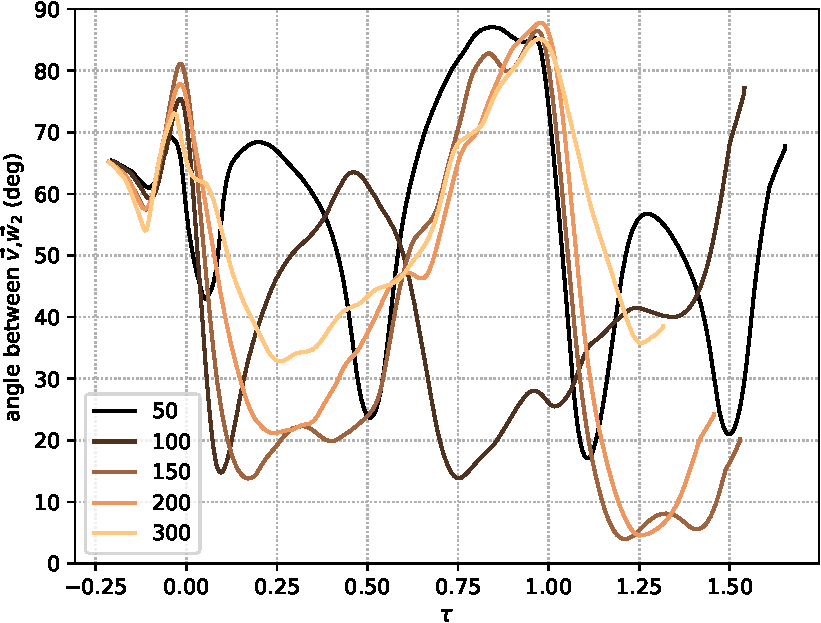
\includegraphics[width=0.8\textwidth]{69_v_angle.pdf}
\caption{Angle between the largest principal component $\vect{w}_2$ and the instantaneous velocity for simulation ID 69.}
\label{fig:pca_angle_v}
\end{figure}

\section{Star formation} \label{sec:where_star_formation}
As shown in the previous section, elongation of material around low clustercentric distances may create grooves in the potential well which lead to angular-momentum transport.
In turn this helps funneling gas towards the center of the galaxy which is squeezed and can cool to create stars.
% TODO non gas run may isolate the role of star formation.
% Ram pressure stripping and tidal interaction can funnel gas into the inner part of the galaxy.
The total content of star forming gas is shown in cyan in Figure~\ref{fig:cold_gas} alongside with the specific star formation rate.
It is interesting to note that for an intermediate mass dwarf, the stripping phenomenon is highly nonlinear.
For example for simulation ID 68, as shown in the corresponding panel in Figure \ref{fig:cold_gas}, the relatively small change of orbit from 150~kpc pericenter to 100~kpc makes the dwarf completely stripped of its reservoir of cold gas.
Due to the stripping, after a burst, star formation stops.
\begin{figure}
\centering
\includegraphics[height=0.95\textheight]{{12.6_sfr_cold_gas}.pdf}
\caption{Specific Star Formation Rate (sSFR) and cold gas (T<$15000$~K) evolution on different orbits.
Different orbits for each galaxy are indicated with shades of brown for the sSFR, and with shades of cyan for the cold gas.}
\label{fig:cold_gas}
\end{figure}

% \citet{Tonnesen2012} argue that pressure in the cluster has a primary role in regulating SF as opposed to the strength of ram pressure.
% NOTE compute cluster gas pressure corresponding to SFR peaks.

% NOTE \citet{Hausammann2019} introduce the parameter $\beta$ defined as the ratio between the ram pressure and the thermal pressure as factor influencing the SF


\subsection{Where do stars form?}
\begin{figure}
\centering
\begin{subfigure}[t]{0.83\textwidth}
\centering
\caption{Simulation ID 71}
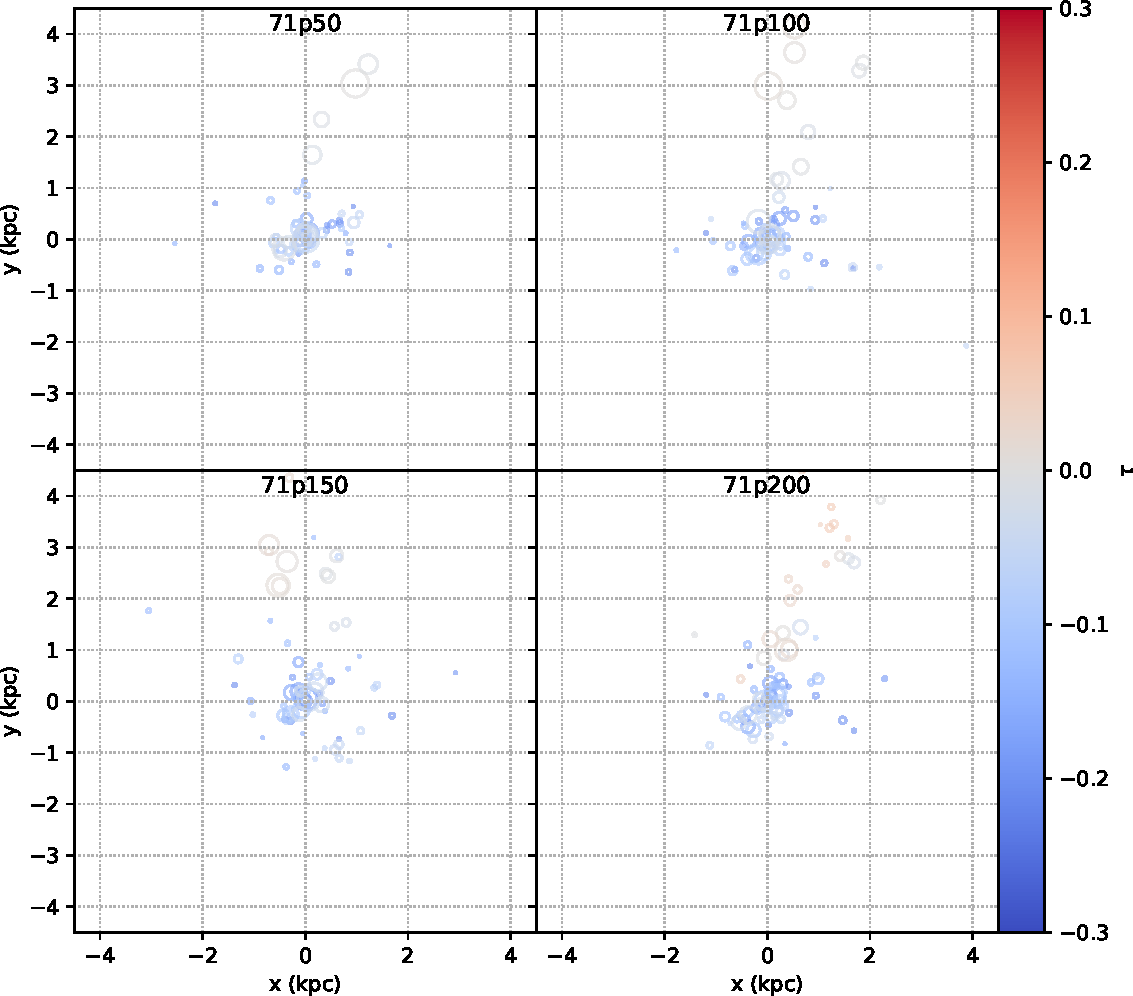
\includegraphics[width=\textwidth]{StarFormationLocation_new71_hollow.pdf}
\end{subfigure}\\%[1.5ex]
\begin{subfigure}[t]{0.83\textwidth}
\centering
\caption{Simulation ID 69}
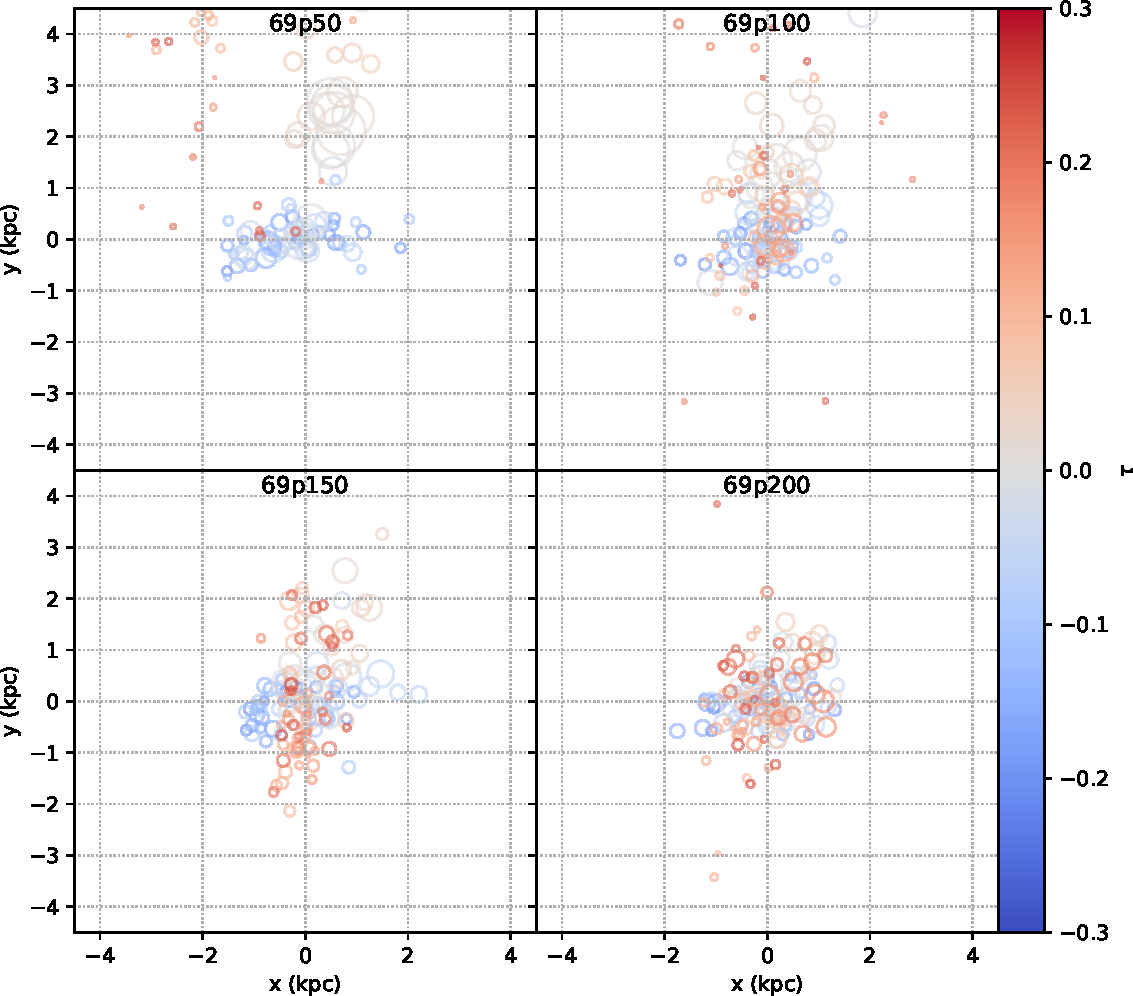
\includegraphics[width=\textwidth]{StarFormationLocation_new69_hollow.pdf}
\end{subfigure}
\phantomcaption
\label{fig:sf_location}
\end{figure}
\begin{figure}[ht]
\centering
\ContinuedFloat % continue from previous page
\begin{subfigure}{0.83\textwidth}
\caption{Simulation ID 41}
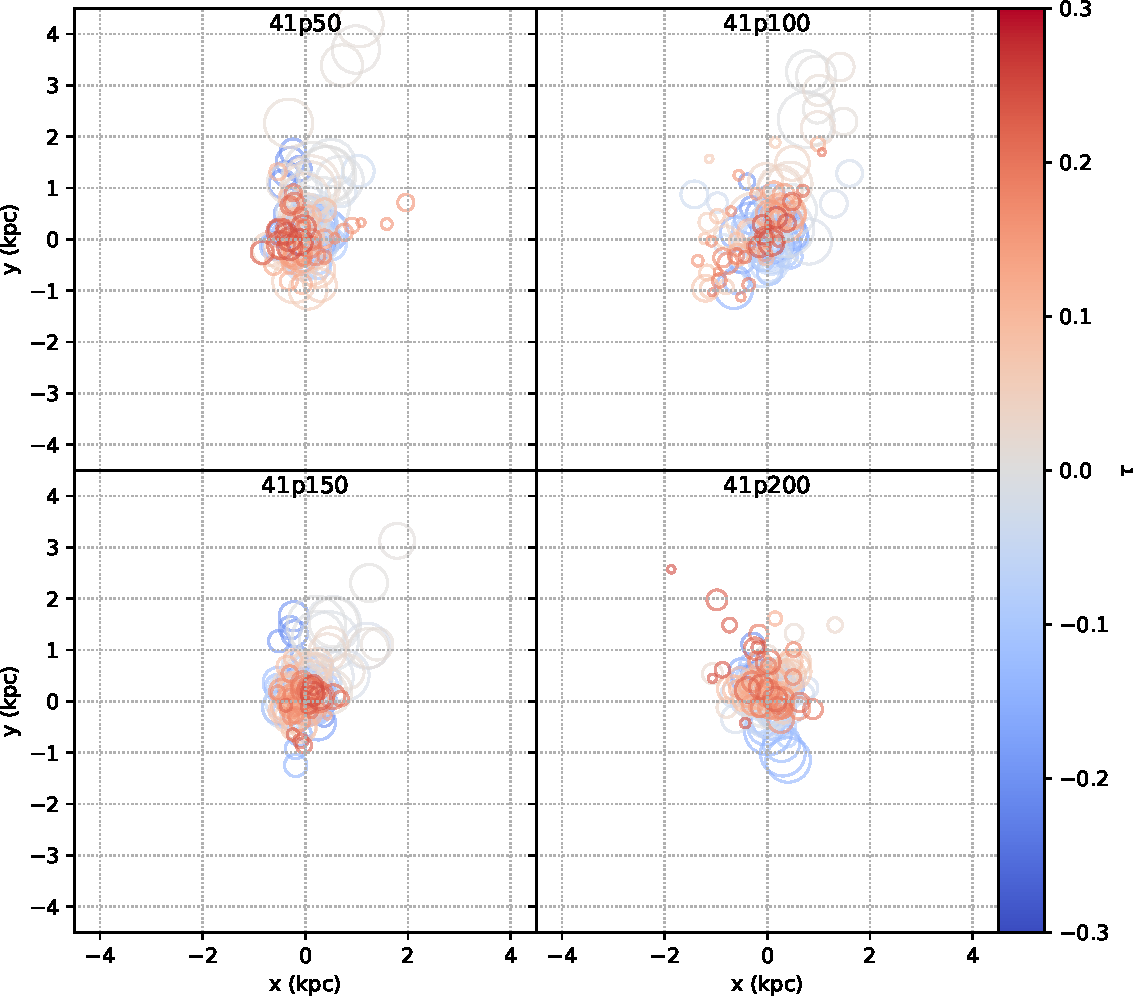
\includegraphics[width=\textwidth]{StarFormationLocation_new41_hollow.pdf}
\end{subfigure}
\caption{Star formation location around first pericenter passage for simulation ID 71, 69 and~41.
Each subpanel corresponds to a different pericenter.
The markers corresponds to the barycenter of the positions of the newly formed stars in each snapshot and are colored according to the distance in time from pericenter normalized with the radial period.
The size of the markers is proportional to the number of stars born between the current snapshot and the previous one.}
\end{figure}
In Figure \ref{fig:sf_location} we show the average position of the star forming particles for each simulation snapshot.
The galaxy is moving in the $-y$ direction (the direction of the instantaneous velocity, see \refsec{sec:MovingBox}) around pericenter.
For each simulation snapshot the number of new stars with respect to the previous snapshot ($10$~Myr before) is counted and their average position in the $xy$ plane is plotted.
\footnote{
We could have computed the star formation rate from the last galaxy snapshot at $z=0$, reading the time of formation of the star particles.
This is the common approach %\citep[e.g.][]{Hausammann2019}
when computing star formation histories of galaxies, and it is observationally motivated.
In fact the star formation history of an observed galaxy is inferred from the photometry and spectrum of the detected starlight.

However, the large amount of star particles lost during the orbit, leads to a large underestimation (of a maximum of 30\% for the most recent bins especially on low mass galaxies on radial orbits) of what has actually happened during the galaxy journey around the cluster.
The method of counting individual star particles newly born is therefore employed.
The choice of a high frequency snapshot cadence plays a fundamental role to this end.
}
In this projection the instantaneous velocity of the galaxy is always directed towards the $-y$ axis.
The ram pressure is therefore pushing in the vertically upwards direction in these diagrams, causing gas to be stripped and stars to be formed in the upper part of the panels.

In correspondence of pericenter passage an intense star formation activity is registered in the gaseous tail.
These galaxies can therefore be defined \emph{jellyfish} galaxies \citep{Ebeling2013}:
the term applies, in fact, to galaxies with star formation activity within the stripped gaseous tails.
Star formation flickers on and off inside the gaseous tails as gas clumps are able to cool, condense and create stars.
This result supports the idea that the jellyfish phenomenon is a relatively short transitory phase of the galaxy along its orbit.

In the three panels of Figure~\ref{fig:sf_location}, three representative galaxies are shown in increasing order of mass.
For the least massive galaxy (simulation ID 71), as confirmed in Figure~\ref{fig:cold_gas}, no stars are formed after pericenter (red markers) because the cold gas is completely stripped by ram-pressure.
However, during the stripping phase new star particles appear in the gaseous tail.
For the intermediate mass galaxy (simulation ID 69), in the radial orbits, the behaviour is similar to simulation ID 71.
Also, a front of newly born star is formed in the center (see panel $69$p$50$) as the gas is compressed and pushed upwards.
For the more circular orbits, stars are continuously formed in the center.
This is a behaviour similar to the most massive galaxy, simulation ID 41, where clumps of gas are detached only in radial orbits.
For the 200 kpc orbit ($41$p$200$) stars are even born in front of the galaxy meaning that for a galaxy so massive a layer of star forming gas is not displaced by ram-pressure even at the leading edge of the galaxy.

\section{Colour Magnitude} \label{sec:CM}
The catalogue of dwarf galaxies in the Fornax cluster, prepared by \citet{Venhola2019}, can be used to directly compare our results with observations.
We build the Color-Magnitude (C-M) diagram with all the simulation snapshots, after computing their SDSS-band colors and magnitude.
We then superimposed it on the results of the observations: as shown in Figure~\ref{fig:g-r} there is a good agreement between the catalogue values and our simulations.
In Fornax, the slopes of the C-M relations are different between the morphologically selected late-type and early-type galaxies.
The relation for the former is rather flat, meaning that the color is not correlated with magnitude, whereas the early-types become redder with increasing total luminosity.

In our simulations, the simulated dwarf galaxies tend to be blue and star-forming when they are near to the cluster center.
Tidal forces and ram-pressure boosts star formation, implying blue luminosities.
The initial mass of the galaxy plays an important role in defining how many times and for how long the galaxy moves between the late-type and early-type regimes.
In fact, if the galaxy gets stripped, it settles on the early-type branch; if instead it can keep its gas, it turns blue again when falling into the cluster.
In particular the lightest galaxy (ID 62) does not survive the first infall yet ending its life in the early-type galaxy realm, independently of the orbit.
On the opposite end of the mass range, the most massive one (ID 41) retains most of its cold gas and, accordingly, its star formation occurs almost steadily, except for the most radial orbit.
Only for the 50~kpc orbit its final location on the C-M diagram is among the early-type galaxies.
Dwarfs on wide orbits, as shown in the 300~kpc pericenter panel of Figure~\ref{fig:g-r}, stay on the blue branch indefinitely unless they become unbound (the condition \eqref{eq:tidal_radius_condition} ceases to be valid), as it happens for the low-mass galaxies.
Figure~\ref{fig:g-r_sfr} confirms that dwarfs rapidly turn red after quenching.

It is interesting to note that, for instance in the 50~kpc pericenter panel, dwarfs jump across the gap between the blue and red branches in between temporally equidistant snapshots.
Given that their color evolves rapidly, the gap between the two branches can be explained: an abundance of dwarfs is not expected in the color interval where their evolution is so quick.

% For the most massive galaxy instead star formation occurs almost steadily (\cf{} Figures~\ref{fig:g-r_sfr} and \ref{fig:cold_gas}).

\begin{sidewaysfigure}
\centering
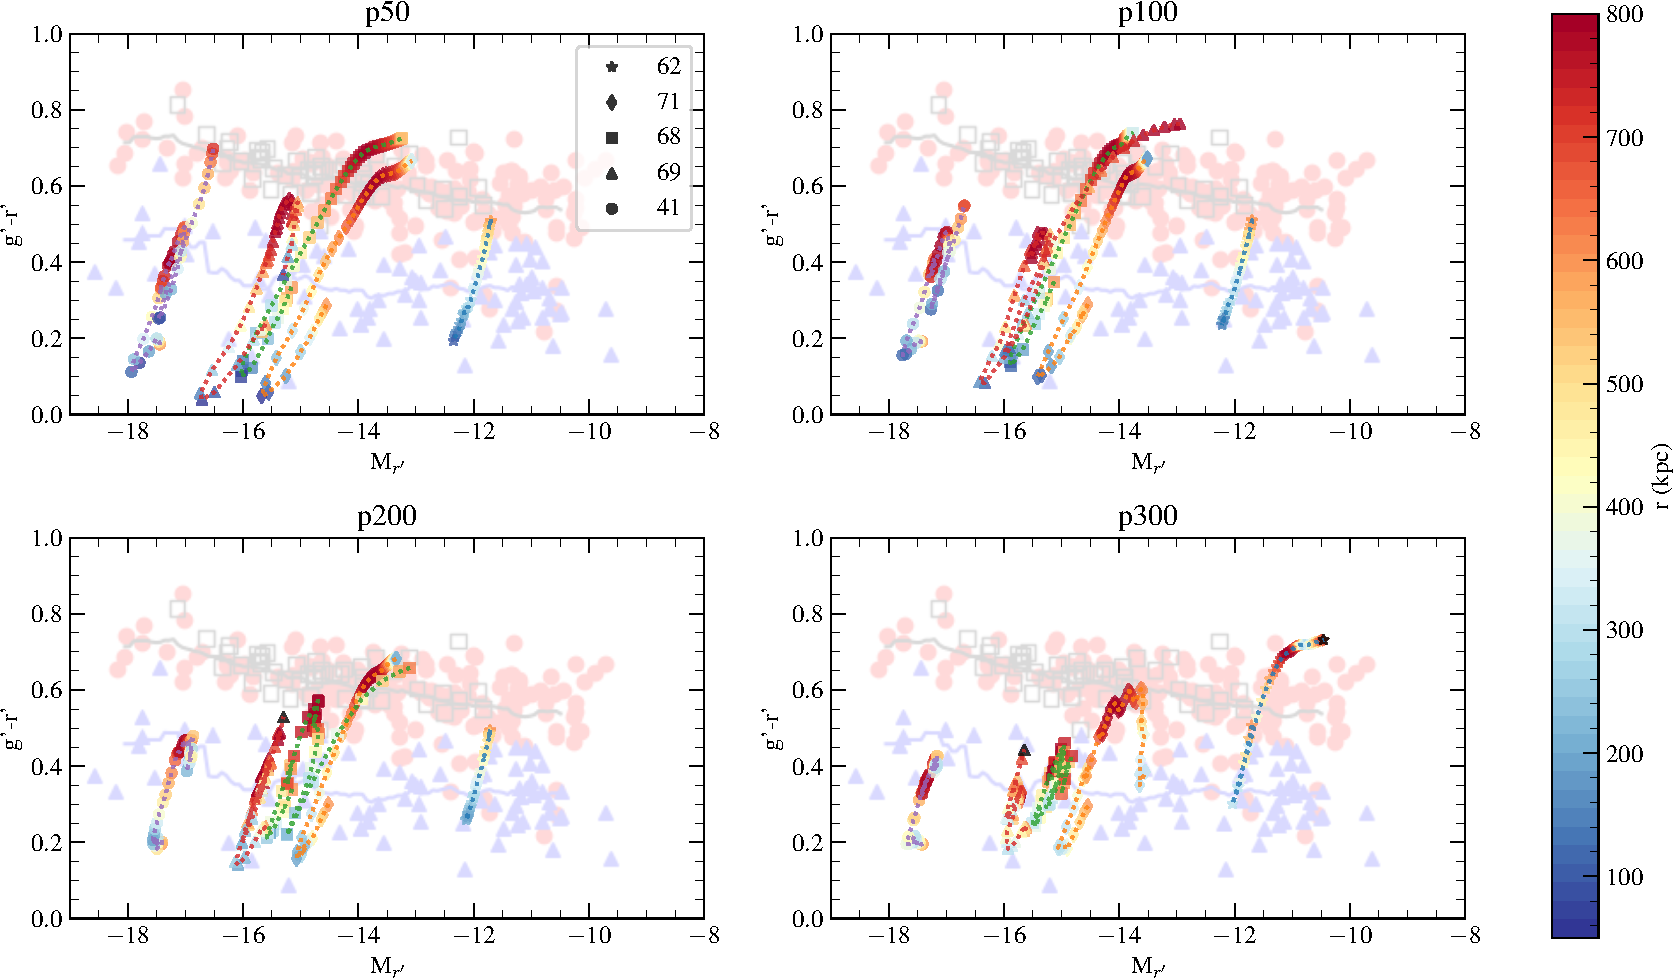
\includegraphics[width=\textwidth]{04.2_color_magnitude_Aku_g-r_rt_criterion_r.pdf}
\caption{SDSS bands colour magnitude diagram of galaxies on different orbits compared to Fornax dwarf catalogue of \citet{Venhola2019}.
% TODO ask permission for the overlay or use catalogue datapoints.
Red and blue colour for the data points in the background represent dwarf elliptical (dE) and late type galaxy respectively, classified by eye on the base of morphology.
Empty squares are nucleated dE.
Data tracks of simulated galaxies are shown overlaid colour coded by the clustercentric radius.
The tracks are limited to bound galaxies \ie{} they are drawn with snapshots for which condition \eqref{eq:tidal_radius_condition} holds.
}
\label{fig:g-r}
\end{sidewaysfigure}
\begin{sidewaysfigure}
\centering
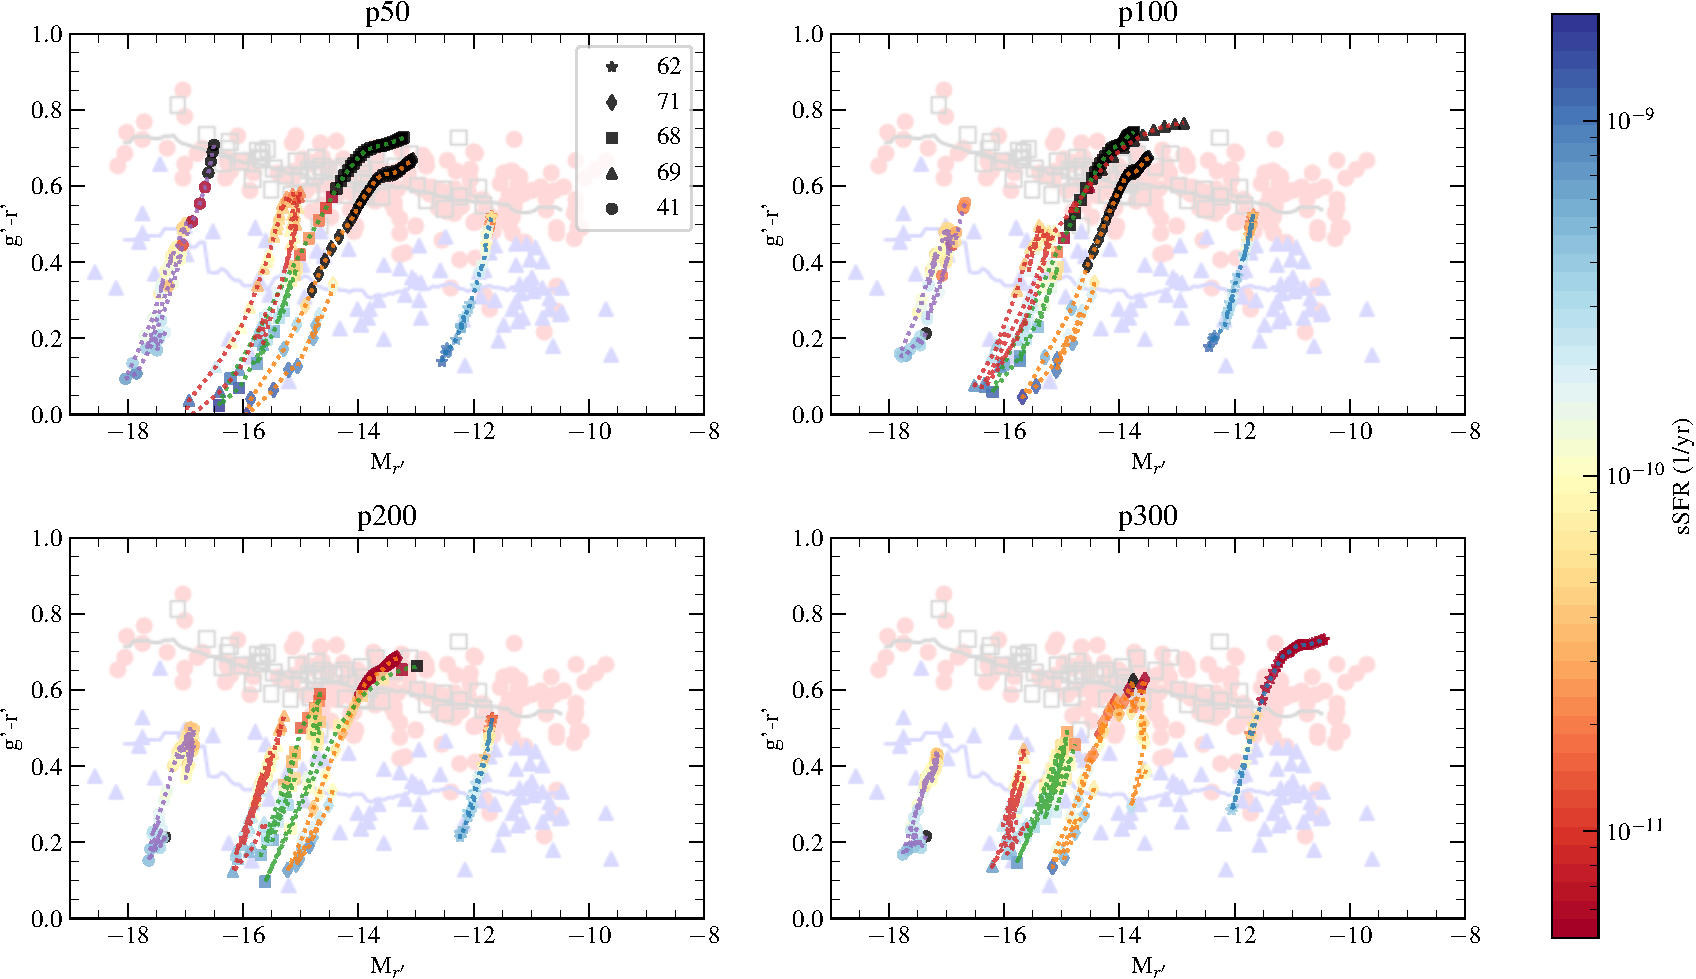
\includegraphics[width=\textwidth]{04.3_color_magnitude_Aku_g-r_rt_criterion_r_sfr.pdf}
\caption{Same as Figure~\ref{fig:g-r}, with point color coded with the specific star formation rate.
Black points are snapshots with no star formation.
}
\label{fig:g-r_sfr}
\end{sidewaysfigure}


\section{HI size mass relation during infall}
\citet{Stevens2019} show how inevitable is the size-mass relation of neutral hydrogen, even during stripping phases.
Our simulations can be checked on the size-mass plane.
As in \citet{Verbeke2017}, we computed the \Hi{} mass by integrating the \Hi{} column density $\Sigma_{\text{\Hi}}$. The radius on the other hand is the major axis of the best fit ellipse on the $1$~\Msun{}~pc$^{-2}$ contour.
%TODO size mass relation
%In Figure \ref{fig:hi_size_mass} we show the behaviour of the gas of a representative dwarf.
% We see that our dwarfs stay on the \Hi{} size-mass relation.

\section{Kinematics}
To correctly compute galaxy kinematics we have to take into account the rotation of the moving box.
The details on how to recover the correct kinematics in our setup are shown in \refsec{sec:correct_kinematics}.

\subsection{Comparison with simulated galaxies in the field}
We compare the specific stellar angular momentum $j_s$ of particles within a sphere of radius $10$~kpc from the center of the galaxy for both a simulation in the moving box as well as for a run in isolation.
We notice in Figure \ref{fig:j_s_moria} an increase of $j_s$ in correspondence to pericenter passages.

The combination of high-velocity newly born stars and the gravitational energy injection given by the cluster at pericenter, result in a spin-up of the galaxy with respect to its evolution in the field.
% TODO metallicity gradient?

\begin{figure}
\centering
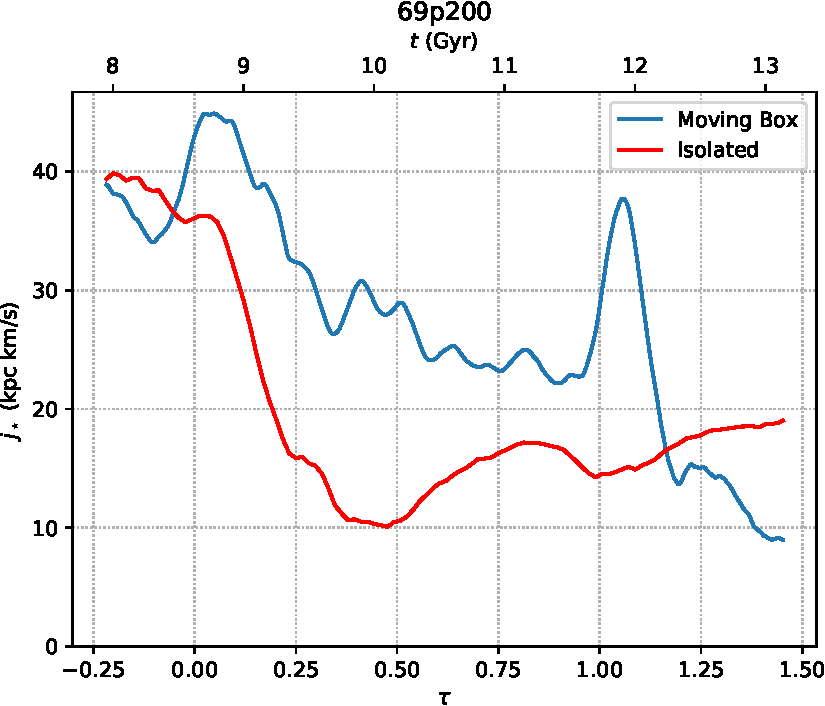
\includegraphics[width=0.8\textwidth]{15.0_angmom_inertial_moria.pdf}
\caption{Comparison between the norm of the specific angular momentum $j_s$ for the simulation ID 69 on a 200 kpc orbit and the correspondent isolated MoRIA run.}
\label{fig:j_s_moria}
\end{figure}

\subsection{Angular momentum and specific angular momentum proxy $\lambda_R$}
We compute the specific stellar angular momentum proxy $\lambda_R$ starting from SPH luminosity-weighted velocity and velocity dispersion maps as defined in \citet{Emsellem2007}: %\citet{Toloba2015}
\begin{equation}
 \lambda_R = \dfrac{\sum_i F_i R_i |V_i|}{\sum_i F_i R_i \sqrt{V_i^2 + \sigma_i^2}}
 \label{eq:lambda_r}
\end{equation}
with $i$ the pixel index, $F_i$ its flux and $R_i$ the distance of the pixel from the galaxy center.
This parameter has been introduced to better capture the spatial information included in the kinematic maps.
As opposed to the classical $v/\sigma$ indicator, $\lambda_R$ has been designed to distinguish between galaxies with kinematically decoupled components (KDC),
which in some cases exhibit large $v/\sigma$ typical of rotation-supported galaxies, despite their rotation being confined to the central regions.

An example of the maps from which $\lambda_R$ is computed for our simulation setup are shown in Figure~\ref{fig:maps_lambda_r}.
The $V_{LOS}$ and $\sigma$ map are computed with SPH interpolation, using the luminosity in $\mathrm{v}$-band to weight the contribution of particles along the line of sight.
Some authors \citep[e.g.][]{Schulze2018,Pillepich2019} use non-weighted quantities taken directly from the particles to compare simulations and observations. %, even if what is observed are luminosity-weighted measures.
This approach makes the comparison with observations more difficult since all the information that we get is luminosity weighted \citep{Walo-Martin2020}.

\begin{figure}[t]
\centering
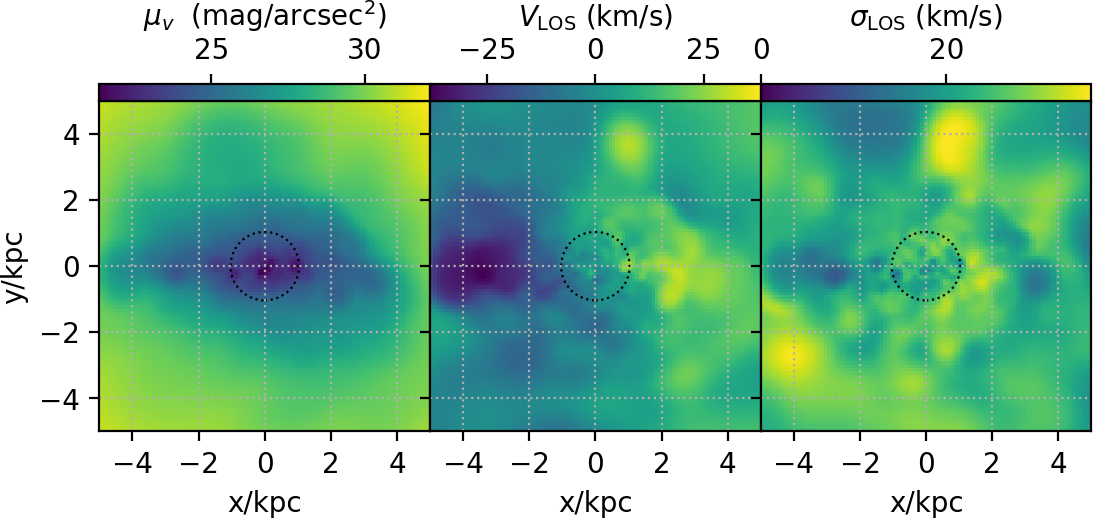
\includegraphics[width=\textwidth]{mu_v_sigma_69p200s60_sideon.png}
\caption{$\mu_\mathrm{v}$ surface brightness map and SPH v-band luminosity weighted maps of line of sight velocity and velocity dispersion $\sigma$ for a snapshot of the simulation ID 69 around first pericenter passage.
The galaxy is projected edge-on, with the angular momentum vector lying on the $xy$ plane.
A dotted circle of radius $R_e$ is shown.}
\label{fig:maps_lambda_r}
\end{figure}

\begin{figure}[h!]
\centering
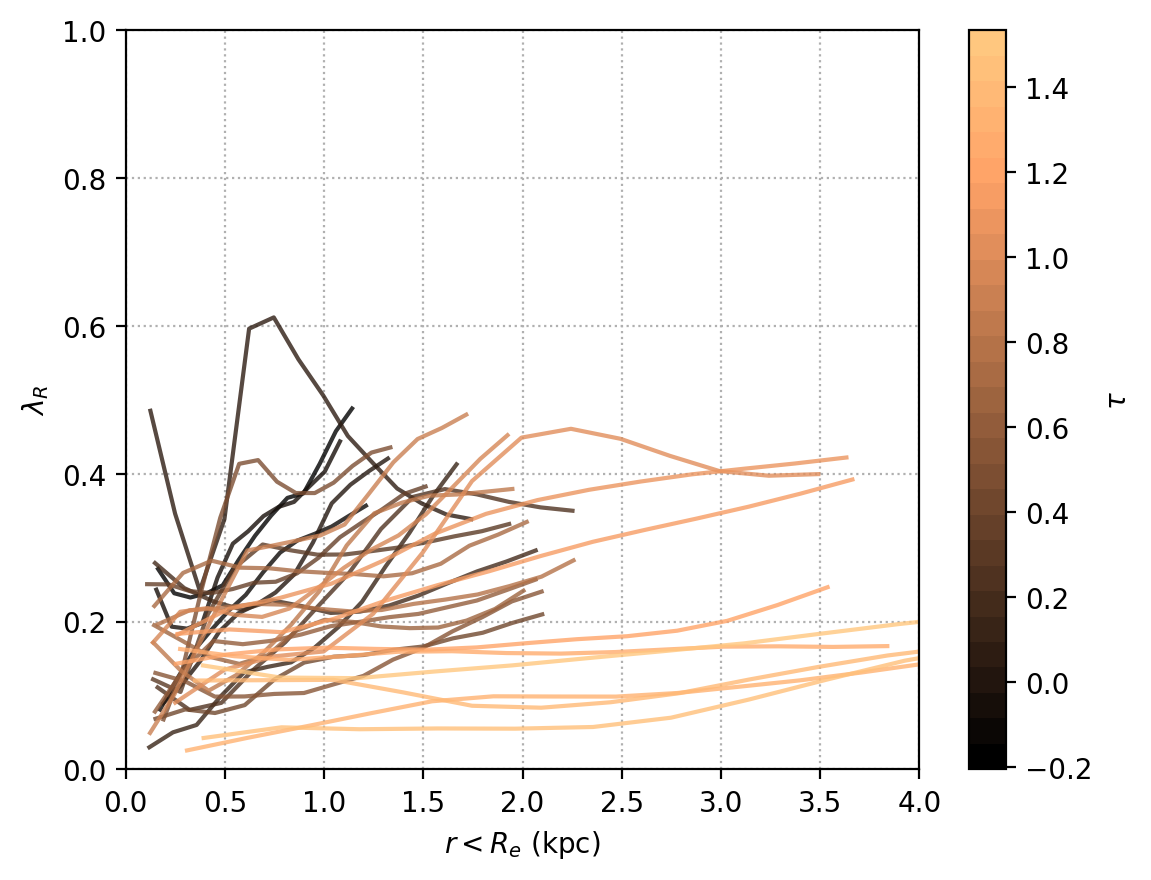
\includegraphics[width=0.8\textwidth]{lambda_r_profile_69p100_each20_up_to_r_e_15bin}
\caption{$\lambda_R$ profiles for ID 69 on a 100 kpc orbit color coded with time normalized by radial period.
The $\lambda_R$ profile is shown up to the corresponding $R_e$.}
\label{fig:lambda_r_profile}
\end{figure}

It is possible to compute the radial profile of $\lambda_R(r)$ including in the summation of eq. \ref{eq:lambda_r} pixels which have distance from the center lower than $r$.
The profile itself and the value $\lambda_R(R_e) = \lambda_{R_e}$ is used to distinguish between fast and slow rotators.
\citet{Emsellem2007} defines galaxies with $\lambda_R < 0.1$ as ``slow rotators'' and those with $\lambda_R>0.1$ as ``fast rotators''. While falling into the cluster, galaxies evolve from being classified as having a fast-rotator profile to slow rotator \citep[\cf{} also][]{Emsellem2011}.
We show an example of the profile in Figure~\ref{fig:lambda_r_profile}, for simulation ID 69 as a function of time.
It is clear that, in a time-frame that is short compared to the lifetime of the galaxy, $\lambda_R$ undergoes significant changes, both locally as a function of radius as well as averaged over the whole galaxy.
In particular, the changes are large enough to cause the galaxy to cross the slow/fast rotator classification threshold.
Also, it is worthwhile to note that the value of $r$ adopted affects whether a galaxy is classified or not as a slow rotator.

There is a complex interplay between $R_e$, $\sigma$ and the rotational velocity while the galaxy is on its orbit.
$R_e$ increases with time whereas velocity dispersion and the rotation velocity at a fixed radius tends to decline.
No single phenomenon can be called to explain the $\lambda_R$ profile behaviour.
The result of this joint evolution is $\lambda_{R_e}$ decreasing with time.

% Obviously this distinction depends on the real inclination of the galaxy, as it appears in the sky. % TODO possible to include inclination in a plot?

It has been shown in the \textsc{SMAKCED} survey of 39 early-type galaxies in the Virgo cluster \citep{Toloba2014, Toloba2015} that the so classified fast-rotator galaxies in the outer region of the cluster rotate faster than the fast rotators in the center of the cluster.
Therefore, in this case, observed specific angular momentum $\lambda_R$ is correlated with cluster-centric distance. % FIXME \citep{Bidaran2020}. citep DEugenio2015
It is indeed hypothesized, that after pericenter passages and a long time in the cluster, galaxies are heated up and transformed into slow rotating dEs.
This scenario is confirmed by our simulations where dwarf irregulars are converted into early-type galaxies, and with time their kinematics is transformed into the one of slow rotators.

In our case, however, the correlation of $\lambda_R$ with clustercentric distance is mild and affected by the very noisy and time-dependent nature of the angular momentum proxy.
For example in simulation ID 69, as shown in Figure~\ref{fig:lambda_r_j_s}, $\lambda_R$ behaviour is very oscillatory %and quite prone to bursty star formation which can abruptly affect its value.
%In our measurements, $\lambda_R$
and fails to distinguish pericenter passages unequivocally.

\begin{figure}
  \centering
  \includegraphics[height=0.9\textheight]{{02.1_lambda_r_vs_js}.pdf}
  \caption{Stellar specific angular momentum proxy $\lambda_R$ and specific angular momentum of star particles $j_s$ for the simulation ID 69 on multiple orbits. The measurements have been taken by observing he galaxy from the plane of the orbit, recreating the condition of a fixed observer.
  Note the relatively stable values of $j_s$ (a conserved quantity) compared to the oscillatory nature of $\lambda_R$, which oscillates by more than $50$\%.}
  \label{fig:lambda_r_j_s}
\end{figure}

\subsection{Relation between $\lambda_R$ and physical angular momentum}
In Figure~\ref{fig:lambda_r_j_s}, in order to compare $\lambda_R$ and the angular momentum of the galaxies in an observationally motivated way, we chose to observe the galaxy from the plane of the orbit, not changing its point of view along its evolution.
Given the spin of the galaxy in correspondence of the pericenter (as shown in the previous section), from this point of view the pericenter passage should be visible in $\lambda_R$ at the highest extent.
In Figure~\ref{fig:lambda_r_j_s}, $j_s$ is the component of the angular momentum perpendicular to the orbital plane.
It is in fact affected by pericenter passages.

It is striking how $\lambda_R$ oscillates along the orbit (\eg{} see panel $69$p$150$) and this highlights how inherently variable $\lambda_R$ is.
It is thus clear that - at least for the class of galaxies we consider - the snapshots in ~\ref{fig:lambda_r_profile} are not representative of the mean value of $\lambda_R$,
and an instantaneous measurement of $\lambda_R$ cannot be used to classify a galaxy as slow/fast, because of the large time-dependent variation.

% \begin{equation}
% \vect{j}_s = \sum_{i\in S} \vect{r}_i\cross\vect{v}_i,\quad \text{where } S\equiv\{k: \norm{\vect{r}_k} < 10 \text{~kpc.}\}
% \end{equation}
% ($\vect{j}_s = \vect{J}_s/M_\star$ where $J_s$ is the total angular momentum and $M_\star$ the stellar mass of the galaxy)
% We compare $\vect{j}_{s}$ with $\lambda_R$ in Figure \ref{fig:lambda_r_j_s}.


\subsubsection{Comparing $\lambda_R$ with observables}
We would like to investigate more the oscillating behaviour $\lambda_R$ shown in Figure~\ref{fig:lambda_r_j_s}.
We tried to use $\lambda_R$ as a starting point to compute the physical angular momentum.
To do so, we try to retrieve an approximate formula for the specific angular momentum which relies on observable quantities:
\begin{equation}
 j_s^* = \lambda_R\, R_e\, \sigma_e
 \label{eq:js*}
\end{equation}
where $\sigma_e$ is the line-of-sight velocity dispersion of star particles measured within an aperture of $R_e$.
For a fair comparison we compute the specific angular momentum $\vect{j}_{se}$ of star particles within $R_e$.
\begin{equation}
  \vect{j}_{se} = \sum_{i\in S} \vect{r}_i\cross\vect{v}_i,\quad \text{where } S\equiv\{i: \norm{\vect{r}_i} < R_e.\}
\end{equation}
% This formula reasonably reintroduces physical dependency.
The relation between $j_{se} = \norm{\vect{j}_{se}}$ and $j_s^*$ is shown in Figure~\ref{fig:lambda_r_j_s_sigma}.
To simplify the treatment, as a first approximation, the snapshot have been rotated edge-on.

\begin{figure}
  \centering
  \begin{subfigure}[t]{0.93\textwidth}
  \centering
  \caption{ID 69}
  \label{fig:lambda_r_j_s_sigma_69}
  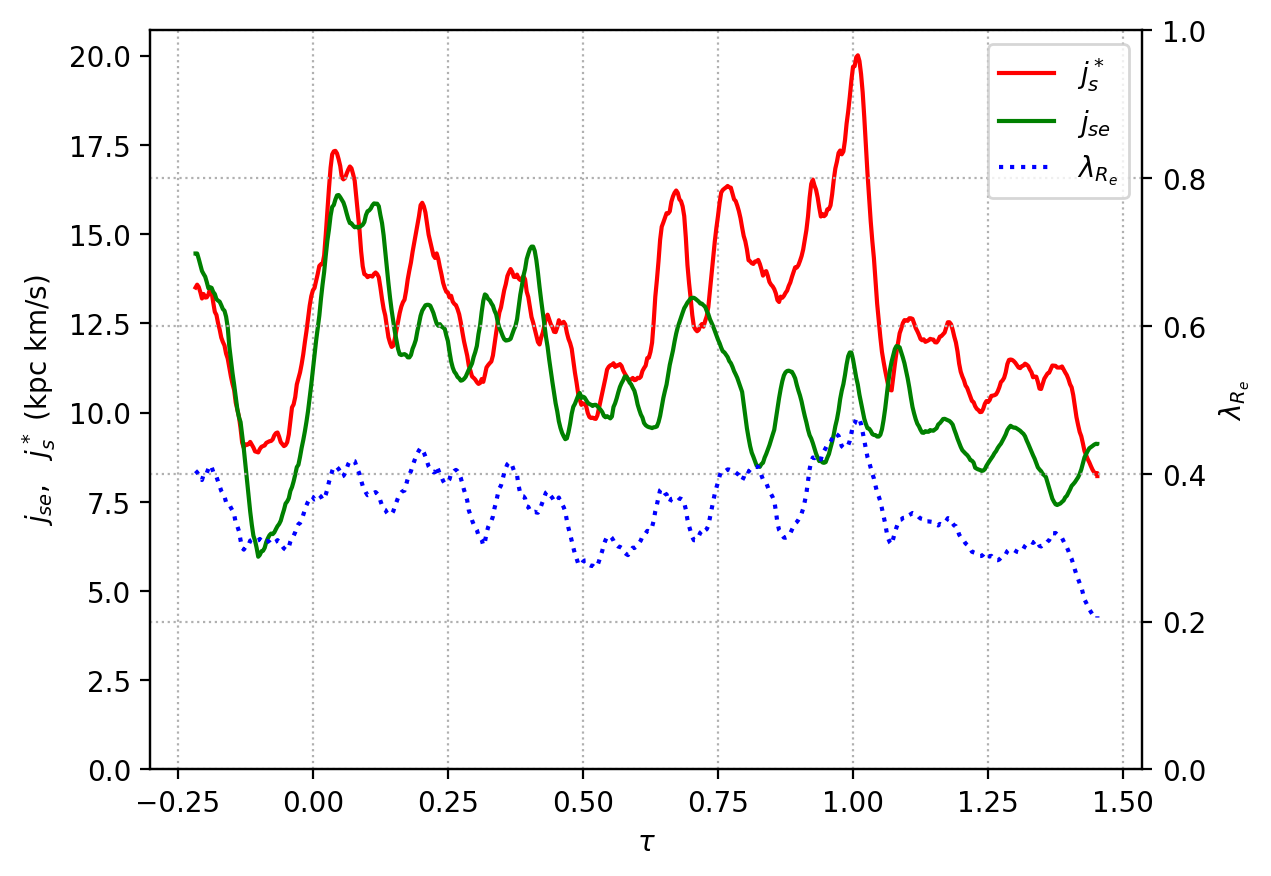
\includegraphics[width=\textwidth]{lambda_r_j_s_69p200r100}
 \end{subfigure}\\
 \begin{subfigure}[t]{0.93\textwidth}
  \centering
  \caption{ID 41}
  \label{fig:lambda_r_j_s_sigma_41}
  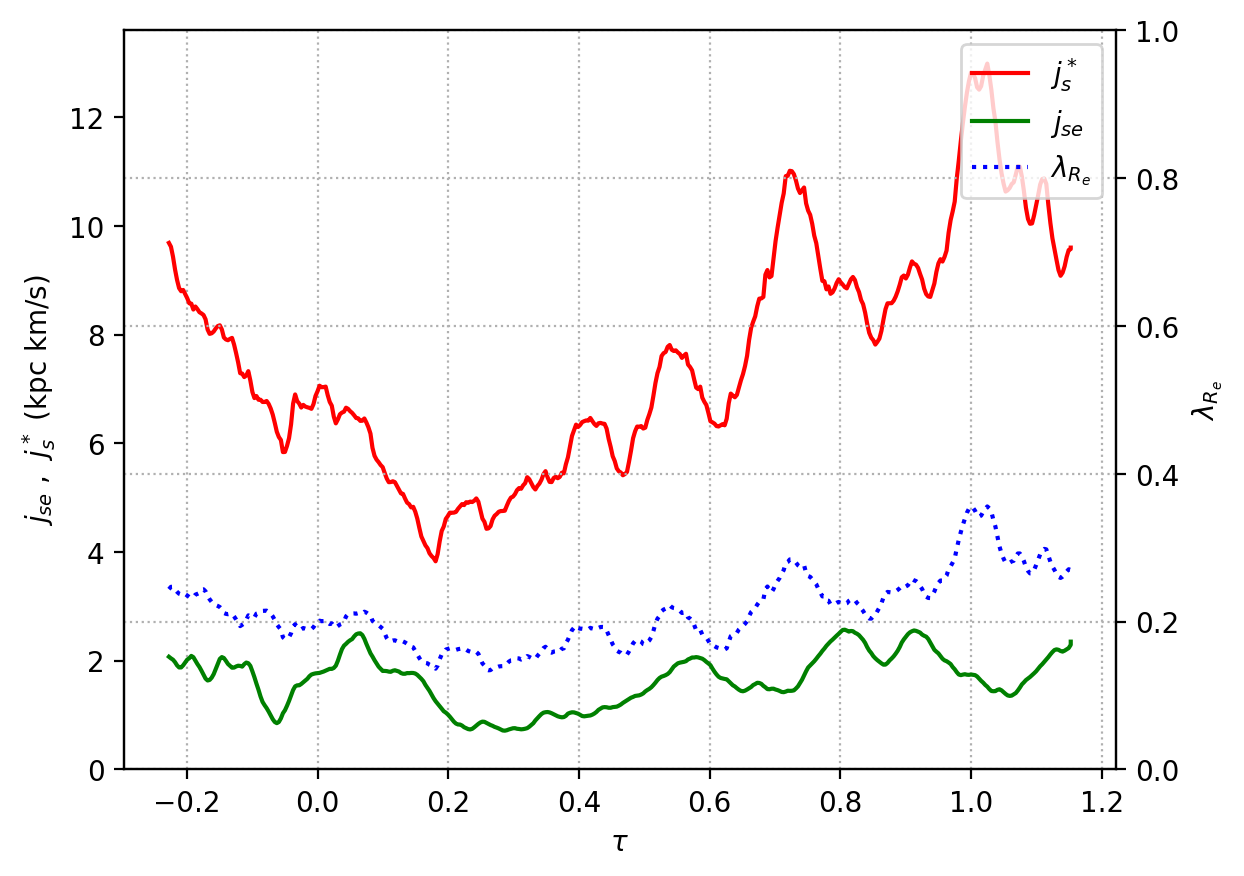
\includegraphics[width=\textwidth]{lambda_r_j_s_41p200r100}
 \end{subfigure}
%  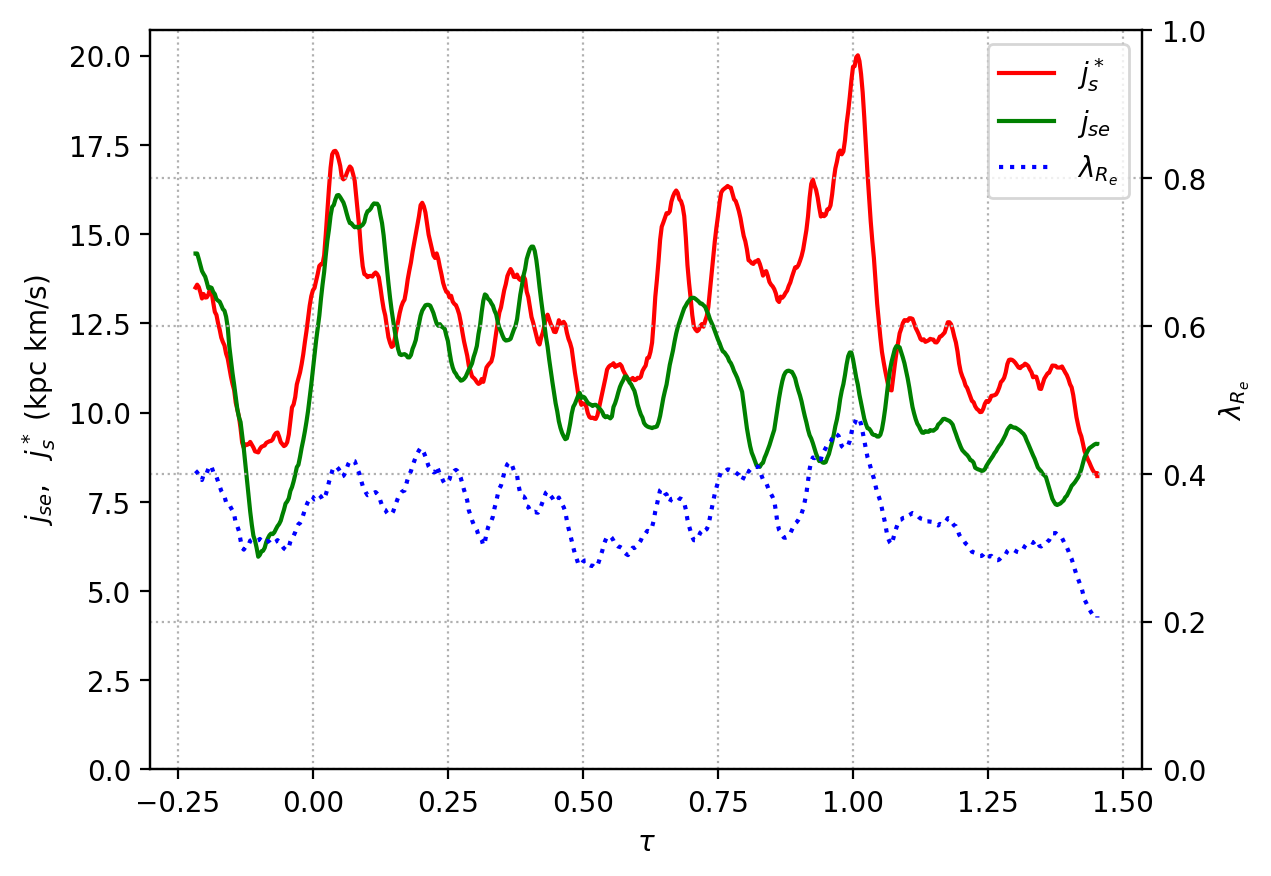
\includegraphics[height=0.42\textheight]{lambda_r_j_s_69p200r100.png}
  \caption{Comparison between specific angular momentum $j_{se}$ and $\lambda_R$ at the effective radius for simulation ID 69 and ID 41 on a 200~kpc orbit.
  $\lambda_R$ is computed viewing the galaxy side-on.
  Curves are smoothed using a rolling average of 0.2~Gyr.}
  \label{fig:lambda_r_j_s_sigma}
\end{figure}

It is interesting to see how for the case of simulation ID 69 in Figure~\ref{fig:lambda_r_j_s_sigma_69} the order of magnitude of $j_s^*$ is strikingly in accord with the measured $j_{se}$ from the particles.
In contrast, for simulation ID 41, there is no correlation.
Given that ID 41 is more massive, we inspected the possibility that by computing both $j_{se}$ and $j_s^*$ within $2 R_e$ a tighter relation between them would emerge.
Figure~\ref{fig:lambda_2r_j_s_sigma} does not support this theory, and the gap between $j_{se}$ and $j_s^*$ increases for the doubled radial limit.

We conclude that in the dwarf-irregular regime covered by our simulations the adapted proxy $j_s^*$ computed in equation \eqref{eq:js*} is not a good tracker of angular momentum.


%As also found by, ... we confirm that it is very sensitive to recent episode of star formation, especially the ones due to gas stripping, where young stars are
% For these reasons in the case of dwarf irregulars it is not a good indicator of the real rotation of the galaxy.

\begin{figure}
  \centering
  \begin{subfigure}[t]{\textwidth}
    \centering
    \caption{ID 69}
    \label{fig:lambda_2r_j_s_sigma_69}
    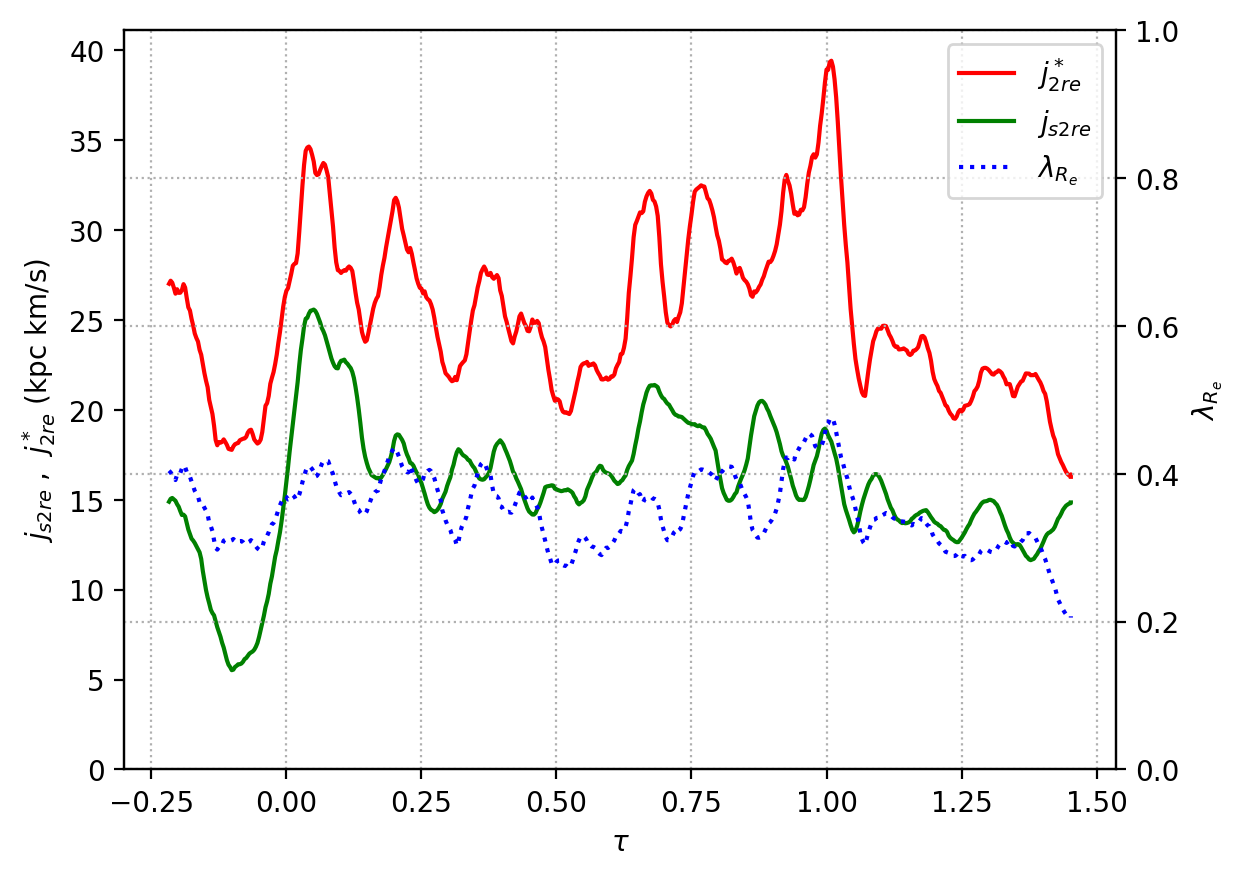
\includegraphics[width=0.93\textwidth]{lambda_r_j_s_69p200r100_2re_only}
  \end{subfigure}\\
  \begin{subfigure}[t]{\textwidth}
    \centering
    \caption{ID 41}
    \label{fig:lambda_2r_j_s_sigma_41}
    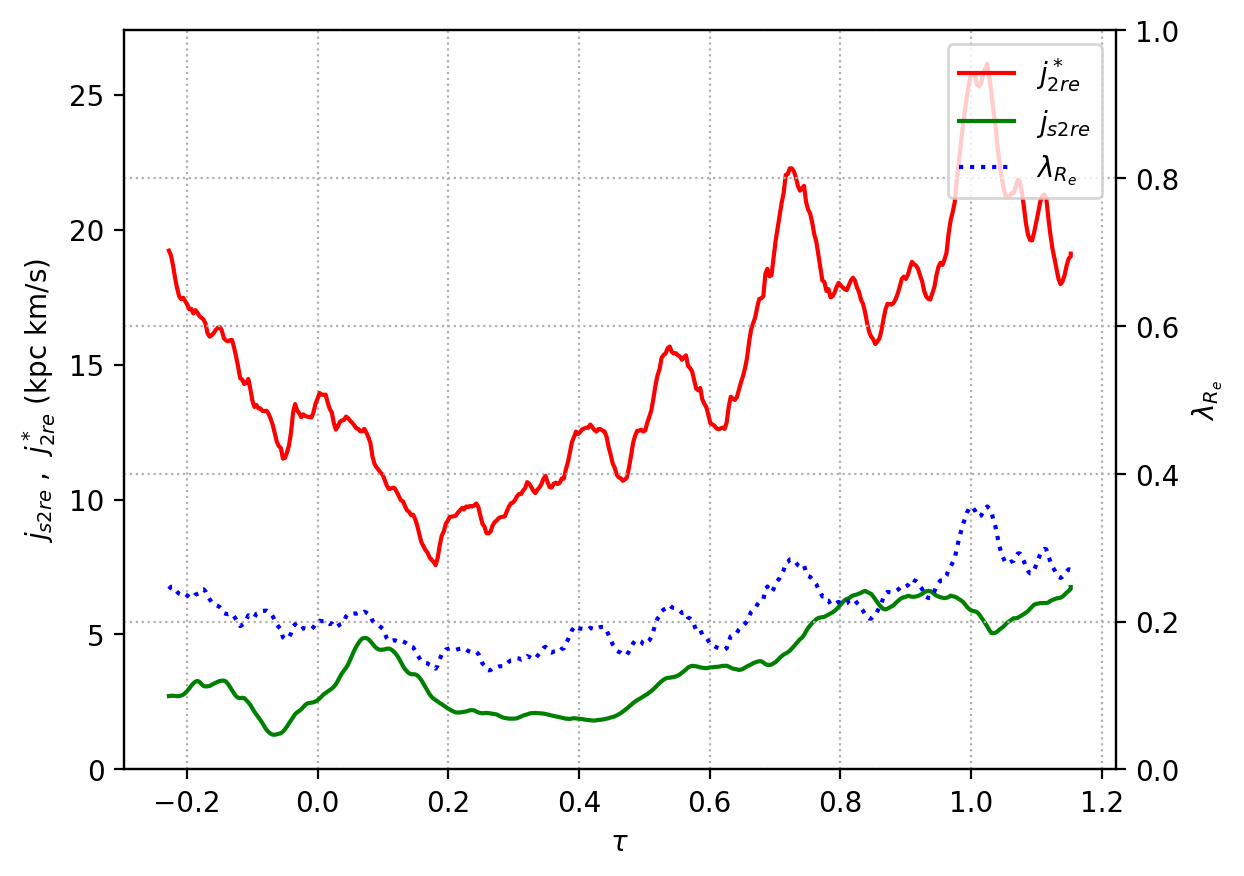
\includegraphics[width=0.93\textwidth]{lambda_r_j_s_41p200r100_2re_only}
  \end{subfigure}
  %  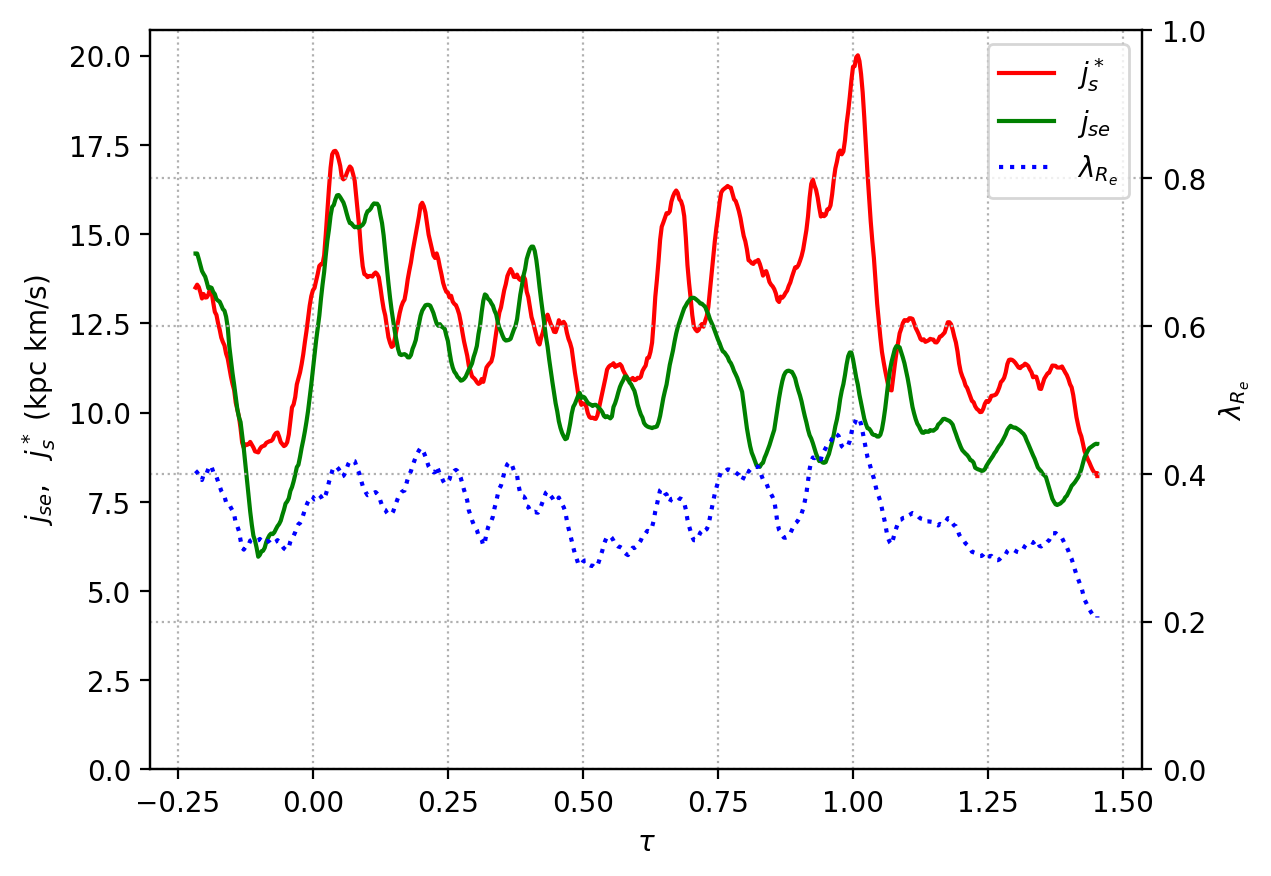
\includegraphics[height=0.42\textheight]{lambda_r_j_s_69p200r100.png}
  \caption{Same as Figure~\ref{fig:lambda_r_j_s_sigma}, but using the limit of $2 R_e$ to compute $j_{se}$ and $\lambda_R$.}
  \label{fig:lambda_2r_j_s_sigma}
\end{figure}

%\section{Conclusions}
%
%\begin{itemize}
% \item $\lambda_R$ is very variable with time in the dwarf irregular regime.
% \item It is sensitive to many things. % FIXME
% \item There can be cases in which depending on the projection and the size of the galaxy, $\lambda_R$ correlates poorly with the physical specific angular momentum.
%\end{itemize}


% \subsection{Magnitude conversion}
% \pynbody{} can be programmed to compute luminosities of stellar particles using
% The built in libraries are from Marico... Padova... %TODO
% To obtain SDSS bands we ued conversion formulas from here, after having computed the magnitudes in Johnson bands.
%

% !TEX root = thesis.tex

{
\cleardoublepage% Move to first page of new chapter
\let\cleardoublepage\relax% Don't allow page break
\noindent \small{Based on: \emph{A tale of two tails: insights from simulations into the formation of the peculiar dwarf galaxy NGC~1427A}, Mastropietro~M., De Rijcke~S., Peletier~R.F. \citet{Mastropietro2021}
}
\chapter[A tale of two tails: on the formation of NGC~1427A]{Insights from simulations into the formation of the peculiar dwarf galaxy NGC~1427A}
\label{ch:ngc1427a}
}

\abstract{
We present a scenario for the formation and the morphology of the arrow-shaped dwarf irregular galaxy NGC~1427A in the Fornax Cluster.
This galaxy shows intriguing stellar and gaseous tails pointing in different directions for which alternative but not conclusive formation scenarios have been proposed in the literature.
We performed $N$-body/SPH simulations of dwarf galaxies falling into a model of the Fornax cluster, exhibiting a jellyfish-like appearance while undergoing ram-pressure stripping.
We noted that some of our models show interesting tail morphologies similar to that of NGC~1427A.
In this way, the peculiar NGC~1427A structure can be studied using models whose stellar and neutral gas photometry and kinematics are in good agreement with the observed ones, without the need of invoking an interaction with a nearby galaxy.
Thanks to the tails, we can identify the requirements for a galaxy to expose such a structure and assess the possible position and velocity of the galaxy in the cluster.
This puts constraints on the orbit of the galaxy, its position in the cluster and the time since its pericenter passage.
From the statistics of identified snapshots following our modelling, we found that the most likely position of the galaxy is around $200$~kpc in front of the cluster center,
travelling towards the cluster with a velocity angle with respect to the line-of-sight direction of around $50$~deg.
This analysis can be useful in future observations of similar galaxies in clusters to characterise their position and velocity in the cluster and their formation.
}


\begin{figure*}
\centering
\includegraphics[width=\textwidth]{NGC1427A-crop.png}
\caption{False-colour image of NGC 1427A, based on HST Advanced Camera for Surveys (ACS) archival data (Proposal ID: 9689; PI: M. Gregg).
The following colour bands were used: blue=475W; green=775W; red=625W+660N (stellar emission was subtracted from the 660N image using a scaled 775W image).
This colour scheme makes the H$\alpha$ emission stand out in red. An asinh stretch was applied to bring out also the faint details.
The inset zooms in on the Northern Clump, showing it to be composed of two loose stellar clusters with embedded \Hii{} emission.
The Northern Clump also appears to be connected to the north-west rim of NGC 1427A's main body via a tenuous stream of stars.
The directions of the \Hi{} tail and towards the Fornax Cluster center are indicated with arrows.
The dotted ellipse is the same as in Figures 1 and 2 of \citet{Lee-Waddell2018} and indicates the shape and direction of the faint outskirts of the galaxy, which are quite distinct from the system's inner, brighter parts.
}
\label{fig:NGC1427A}
\end{figure*}
The distorted optical appearance and gaseous tails and overall jellyfish-like morphology --~barring currently active star formation in the gas tails~-- of NGC~1427A (Figure~\ref{fig:NGC1427A}) seems to be straightforwardly and satisfactorily explained by ram-pressure stripping in conjunction with cluster tidal forces.
In particular, as has been explored more in detail in Chapter \ref{ch:sim_results}, star formation flickers on and off inside the gaseous tails of simulated ram-pressure stripped dwarf galaxies as gas clumps condense and disperse again.
This gives the label ``jellyfish galaxy" a transient and possibly recurrent quality.

To correctly interpret the available data, it is of prime importance to be able to reliably identify the dominant transformation process for this galaxy.
With this goal in mind, we compare recent \Hi{} and optical data of NGC~1427A with a suite of dwarf galaxy simulations, set in a Fornax Cluster environment.

In the next section, we give a short overview of the observed properties of NGC~1427A and focus on those that are considered most relevant for elucidating its origin and evolution.
The methodology behind the comparison of these simulations with the observations is discussed in Section~\ref{sec:results}.
We conclude with a discussion of the main results in Section~\ref{sec:discussion}.


\section{Observed properties of NGC~1427A} \label{sec:observations}
\begin{figure*}
\centering
\begin{subfigure}[b]{0.49\textwidth}
  \centering
  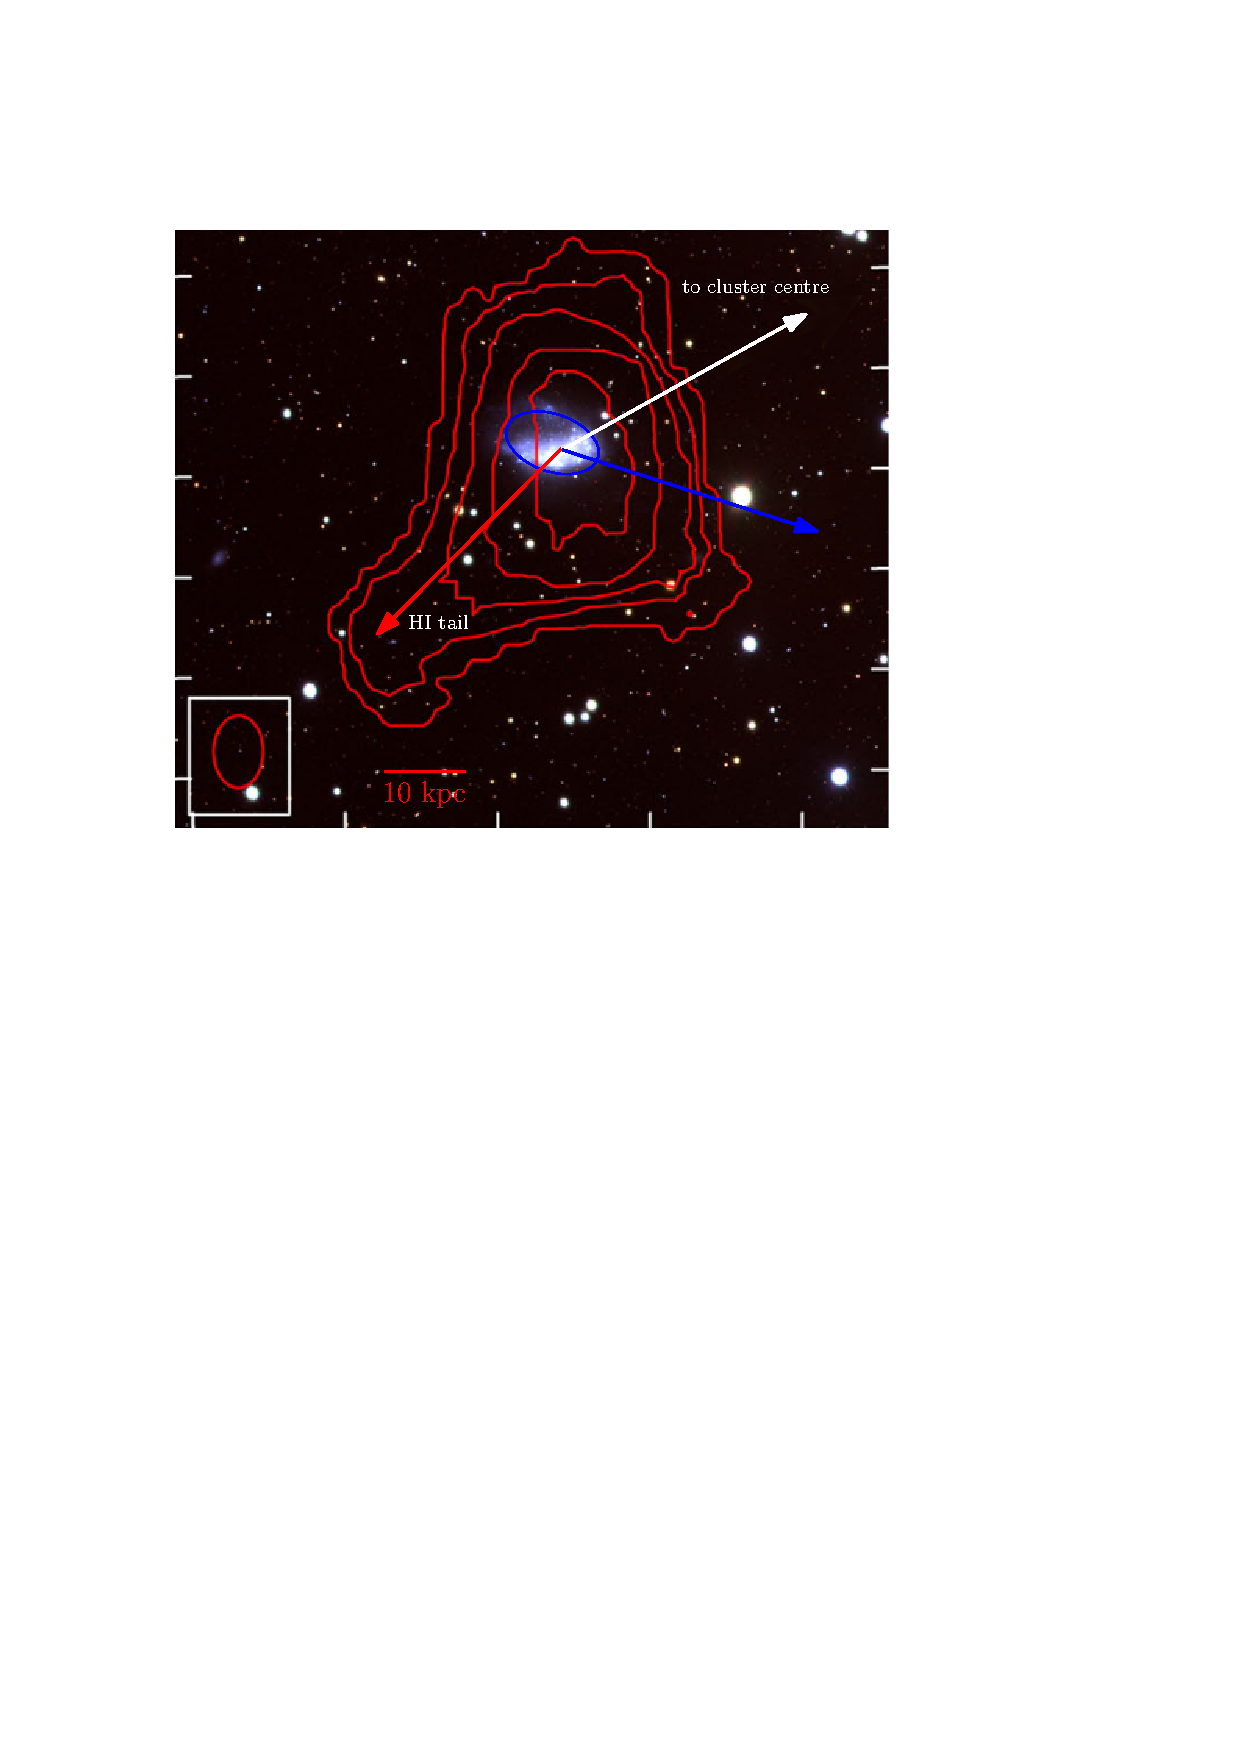
\includegraphics[width=\textwidth]{NGC_LIKE/ngc_location_scale.pdf}\\[3ex]
  \caption{}
  \label{fig:hi_contours}
\end{subfigure}
% \hfill
\begin{subfigure}[b]{0.49\textwidth}
  \centering
  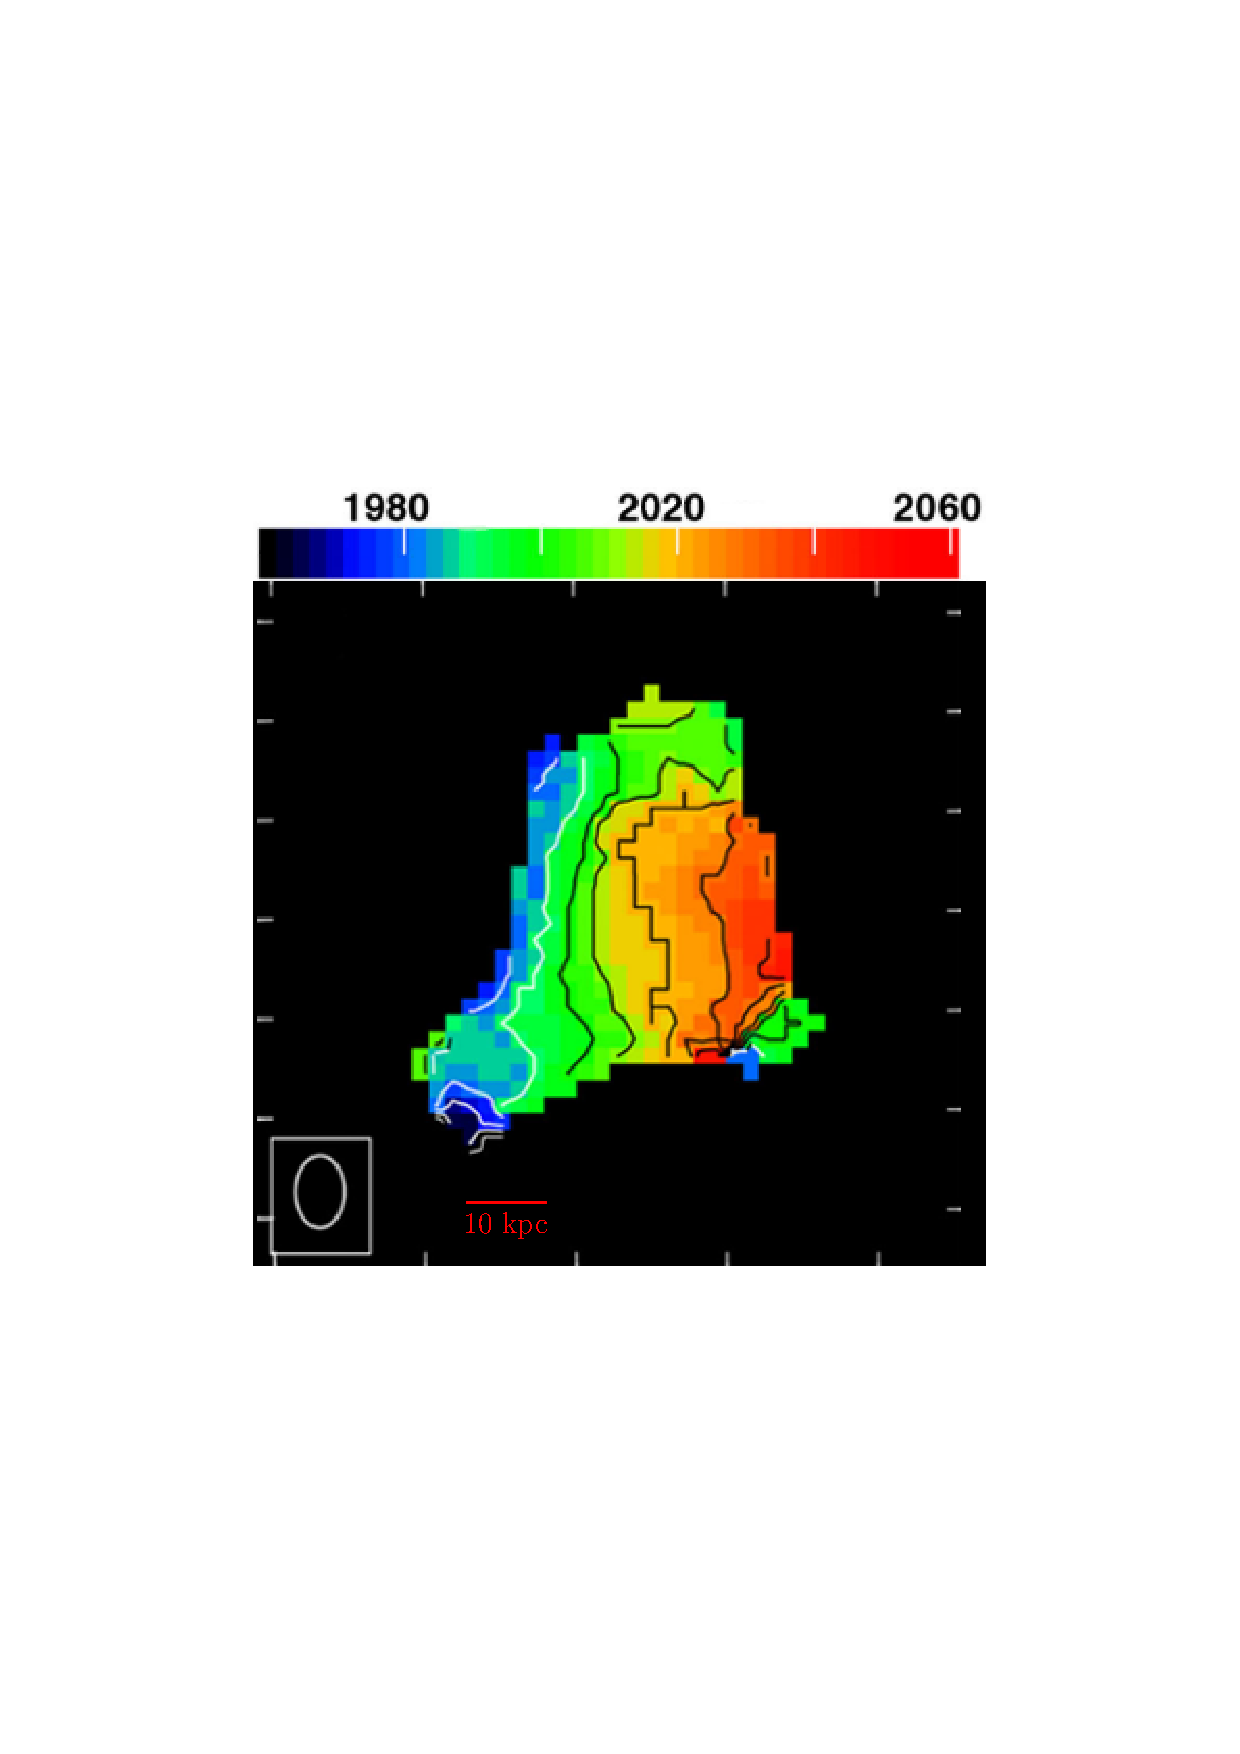
\includegraphics[width=0.9\textwidth]{NGC_LIKE/kin_scale.pdf}\\[3ex]
  \caption{}
  \label{fig:hi_kin}
\end{subfigure}
\begin{subfigure}[b]{0.6\textwidth}
  \centering
  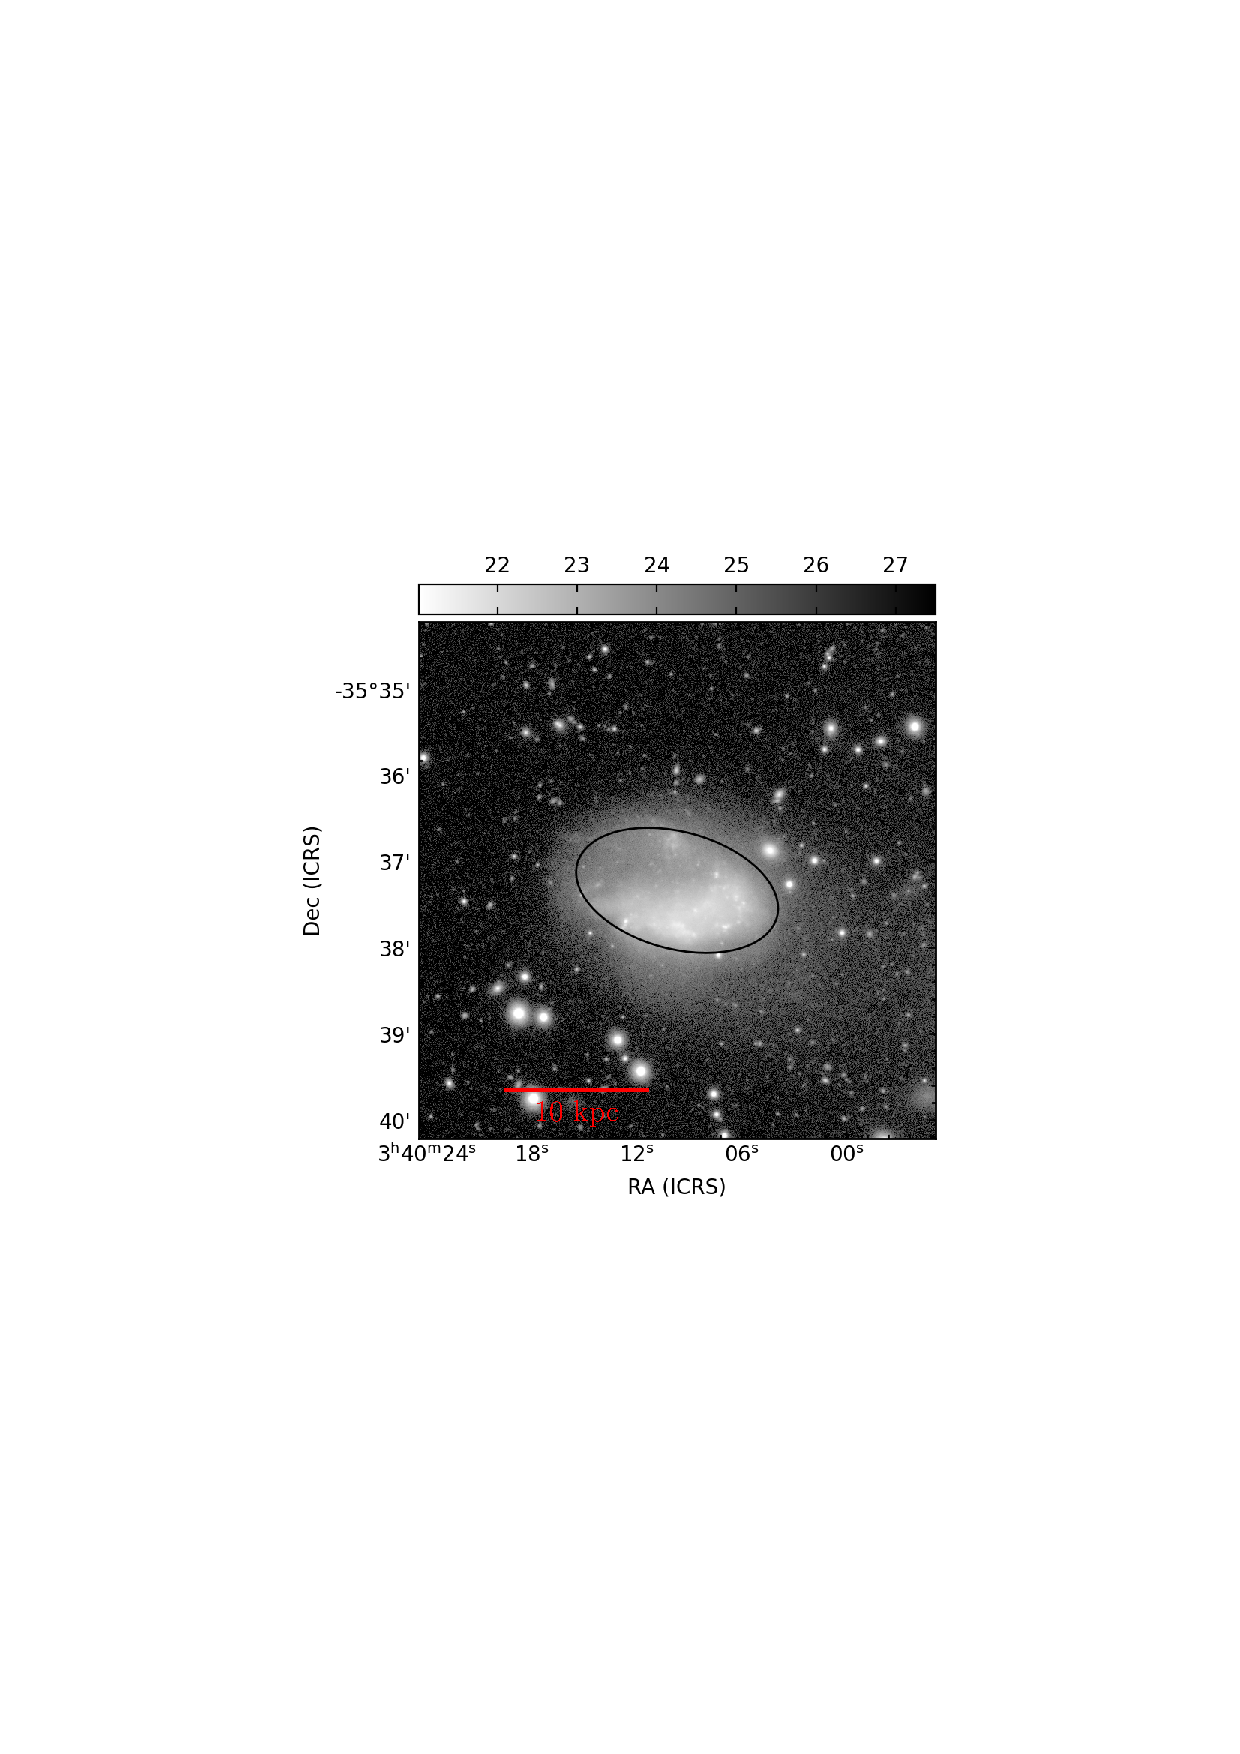
\includegraphics[width=\textwidth]{NGC_LIKE/ngc_tide_scale.pdf}%\\[3ex]
  \caption{}
  \label{fig:r_band}
\end{subfigure}
% \hfill
\caption{
Images of NGC~1427A from \citet{Lee-Waddell2018} for illustrative purposes:~(a) VST image with overplotted in red contours of constant \Hi{} column density at levels $(0.5, 1, 2, 5, 10) \times 10^{20}$~amu~cm$^{-2}$;
(b) gas kinematics (recessional velocity in km/s)
(c) $r'$-band image (in mag/arcsec$^2$).
A length scale at the assumed cluster distance is indicated in red.}
\label{fig:NGC_OBSERVATIONS}
\end{figure*}
NGC 1427A is a gas-rich dwarf irregular galaxy in the Fornax Cluster.
Recessional velocity measurements indicate that NGC~1427A is moving with a line-of-sight velocity of around 2028 km/s \citep{Bureau1996, Schroder2001}.
Accordingly, if we assume NGC~1399 to be the cluster center, NGC~1427A travels away from us at a projected speed of around 700~km/s relative to the cluster center. NGC 1427A has a projected distance of 137 kpc from NGC|1399\footnote{The angular separation is 1373$\arcsec$ = 137~kpc, throughout the paper, we assume a fiducial distance of the cluster center of 20~Mpc.}.

A false-colour HST image of the galaxy is shown in Figure~\ref{fig:NGC1427A}.
The inset of Figure \ref{fig:NGC1427A} zooms in on the Northern Clump, showing it to be composed of two loose stellar clusters with embedded \Hii{} regions.
The Northern Clump also appears to be connected to the north-west rim of NGC~1427A's main body via a tenuous stream of stars.
The directions of the \Hi{} tail and towards the Fornax Cluster center are indicated with arrows.
The dotted ellipse is the same as in Figures 1 and 2 of \citet{Lee-Waddell2018} and indicates the shape and direction of the faint outskirts of the galaxy.
We interpret these low-surface-brightness stellar features, which point towards the north-east and south-west (effectively captured by the ellipses in Figure~\ref{fig:NGC1427A} and \ref{fig:r_band}), are quite distinct from the much brighter inner regions of the galaxy's main body, as tidal features.
The Northern Clump, which we discuss in detail in Section~\ref{NC1427A}, may be associated with these tidal features.

\citet{Chaname2000} presents a lower limit for the dynamical mass of NGC~1427A using a rigid-body rotation model: $M_{\mathrm{dyn}}~>~(9\pm 3)\times 10^9 M_\odot$.
Following the calibrated empirical relation of \citet{Taylor2011}, the stellar mass estimated by \citet{Lee-Waddell2018} is $M_{\star} \approx 10^9 M_\odot$ while its total \Hi{} mass is determined to be $M_{\mathrm HI} = (2.1 \pm 0.2) \times 10^9 M_\odot$.
The galaxy has a conspicuous \Hi{} tail, containing about $10$ per cent of all \Hi{} gas in NGC~1427A, pointing towards the south-east as well as stellar tidal extensions along a north-east to south-west axis.
In other words:~the gaseous and stellar extensions are almost perpendicular to each other.
NGC~1427A was not detected in CO emission, providing an upper limit on its molecular gas mass of the order of $M_{\mathrm H_{2}}~\sim 10^8$~M$_\odot$ \citep{Zabel2019}. These authors report the detection of a single 3~mm continuum source without an optical counterpart but its nature remains unclear.
A distinct young stellar clump is visible in the northern rim of the galaxy.
On high-resolution images, this clump, the rim, as well as the galaxy's main stellar body are resolved into many individual OB associations and clusters, some with accompanying H$\alpha$-emission \citep{Hilker1997, Sivanandam2014}.
Clearly, star formation proceeds in many dispersed small bursts.

Various hypotheses regarding the evolution of NGC 1427A, and especially its extraordinary configuration of tails, have been proposed.
These include recent interactions with other nearby galaxies \citep{Cellone1997}, a merger with an object that now forms the northern stellar clump \citep{Lee-Waddell2018},
the tidal interaction with the cluster potential, and ram-pressure stripping of its gas by the cluster hot gas halo \citep{Chaname2000, Mora2015}.
%This galaxy has been described by \citet{Laustesen1987} with this expression \emph{"It contains a large number of gaseous and luminous clusters, which partially form a ring towards the western edge of the galaxy”}. \citep{Cellone1997}
%What \sven{is especially striking} regarding NGC 1427A is the relative direction of its twin stellar and gaseous tails\sven{:~they are almost perpendicular to each other}.
% Various hypothesis on the formation scenarios have been proposed \cite{Hilker1997, Cellone1997, Chaname2000, Mora2015, Lee-Waddell2018}:
% tidal interactions with other nearby galaxies, tidal interaction with the cluster potential and ram pressure stripping of its gas by the cluster hot gas halo.

To try and identify the environmental processes acting on NGC~1427A, we first selected those properties of this dwarf galaxy that were most likely to be indicative of those processes and not of internal effects. Those are:
\begin{enumerate}
    \item the direction towards the Fornax cluster centrum,
    \item the direction of the axis of the stellar tidal extension,
    \item the direction of the \Hi{} tail.
\end{enumerate}
These parameters are most tightly linked with NGC~1427A's orbit through the Fornax Cluster and are expected to be relatively insensitive to the accidents and vagaries of its evolution before its acquisition by the cluster.

Thus, our analysis differs from that of \citet{Lee-Waddell2018} where the ram-pressure hypothesis is discussed based on stellar colour and galaxy morphology information.
Their new data indeed rule out a ram pressure origin for the optical appearance of the galaxy, but they leave open the question whether ram pressure may have played a role in the formation of the \Hi{} tail.

% We carried out a morphological search throughout our suite of simulations to isolate snapshots with the above properties respecting.% which can be useful to characterise the effects leading to such peculiar morphology.
% We found that the main effects generating peculiar morphology are indeed the combination of galaxy rotation, ram pressure and tidal interaction close to the cluster center.
% % It's clear also (see Figure \ref{fig:3dview}) that gaseous and stellar components react differently to the main stretching factors: ram pressure and gravity gradient.

% Instead, we take verbatim the indication from the \Hi{} map (their Figure 3): \emph{the neutral hydrogen galactic tail is a direct indication of the direction of motion of the galaxy}.
% Moreover, the \Hi{} velocity distribution as measured by \citet{Lee-Waddell2018} shows that the \Hi{} tail in its west part is receding more than the eastward part.
% As opposed to a rotation, we interpret the \Hi{} LOS velocity gradient as a direct indication of the stripping process. % \Hi{} 21 line profiles in \cite[p.63]{Bureau1996} do not show a double horn profile.



% \todo{
% % Possible bibliographic items to take into account: \citet{Bournaud2004}

% Simulation related bibliographic items to take into account: \cite{Joshi2018, Joshi2020}
% }

% \section{Observations}
% \cite{Lee-Waddell2018}
% SFR = 0.065 \Msun yr$^{-1}$ and $\log$(sSFR) = -10 from \cite{Sivanandam2014}
% \begin{figure}
% 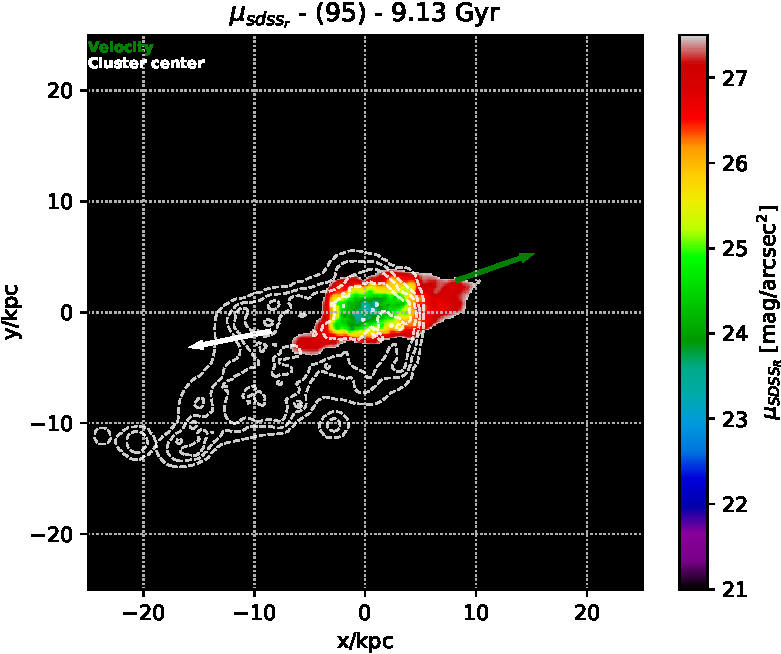
\includegraphics[width=\columnwidth]{69p100_0095_sb-crop.pdf}
% \caption{Surface brightness map with superimposed \Hi{} density contours with 5 equidistant in log-scale levels from $10^{17}$ to $10^{22}$ atoms/cm$^2$.}
% \label{fig:sb}
% \end{figure}

\section{Simulations} \label{sec:simulations}
\begin{figure}
\centering
\begin{subfigure}[b]{0.49\textwidth}
 \centering
 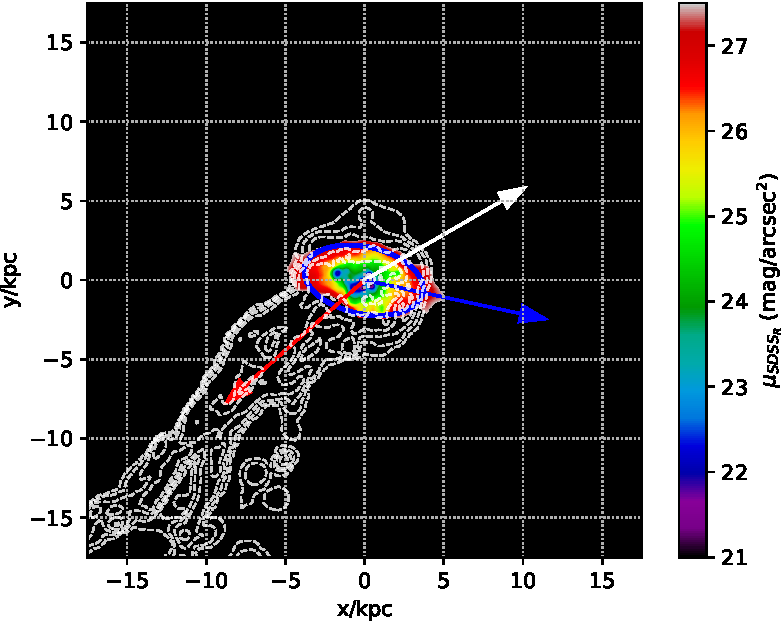
\includegraphics[width=\textwidth]{NGC_LIKE/SB.pdf}
 \caption{}
 \label{fig:sb_arrows}
\end{subfigure}
 \hfill
  \begin{subfigure}[b]{0.5\textwidth}
  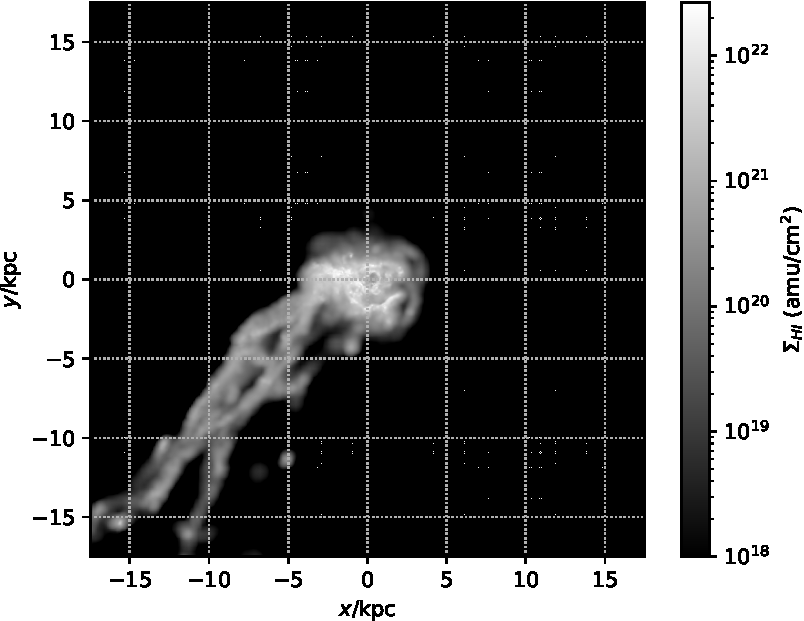
\includegraphics[width=\textwidth]{NGC_LIKE/HI.pdf}
  \caption{}
  \label{fig:sim_hi_density}
\end{subfigure}
\hfill
\begin{subfigure}[b]{0.5\textwidth}
  \centering
  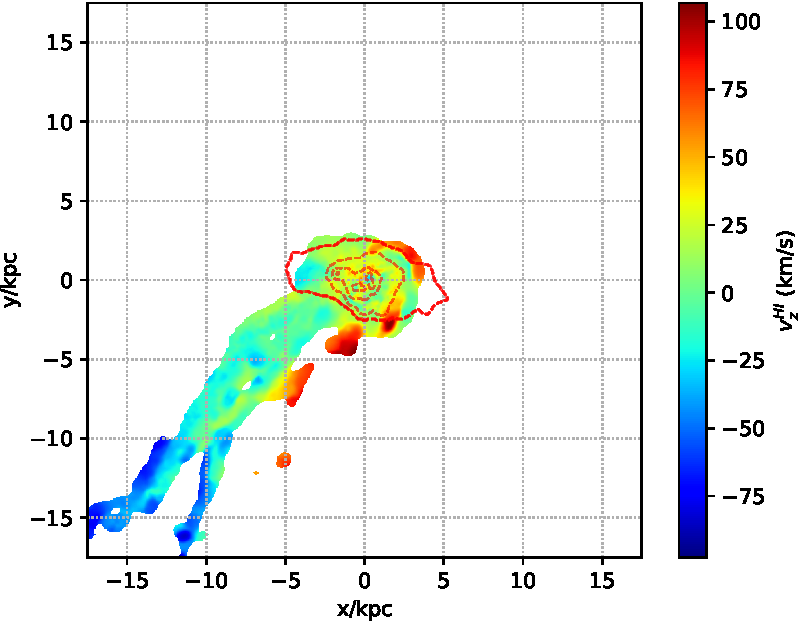
\includegraphics[width=\textwidth]{NGC_LIKE/HI_VEL.pdf}
  \caption{}
  \label{fig:sim_hi_kin}
\end{subfigure}
 \vfill
\caption{A simulation snapshot (ID 68, see Table \ref{tbl:sim}) on an orbit with 100 kpc pericenter distance, showing stellar tidal and gaseous stripped tails.
(a) $r'$-band surface brightness with \Hi{} column density contours as seen from a point of view for which the projected cluster-centric distance $r_p = 77$ kpc and the recessional velocity $-793$ km/s.
\Hi{} contours are drawn at column density levels [$10^{17}, 10^{18}, 10^{19}, 10^{20}, 10^{21}$]~amu~cm$^{-2}$. The white arrow points towards the cluster center, whereas the blue and the red arrows are the computed orientation of the stellar tail and the gaseous tail respectively, see Section \ref{sec:morphological_quest}.
%(same as \citet{Lee-Waddell2018})
(b) The column density of the neutral hydrogen, highlighting clumpy blobs of stripped \Hi{}.
(c) SPH map of the \Hi{} velocity field where the \Hi{} tail in its rightmost part is receding more than the more detached part.
For reference, the [22, 24, 26, 28]~mag/arcsec$^2$ isophotes are shown as dashed red contours.
We stress that our Fornax cluster dwarf galaxy simulations were not designed to reproduce all the details of this particular galaxy. Nonetheless, remarkable similarities can be found.}

\label{fig:selected_snapshot}
\end{figure}

The simulations used in this chapter are described in full details in \refsec{sec:fornax_sim}.
We stress that they have not been set up to mimic NGC~1427A in any particular way. Therefore, not all details can be expected to exactly match with observations.
Nonetheless, these simulations provide valuable insights not only into the phenomena at play but, more importantly, they can be used to infer the most likely current orbital phase of the galaxy.


\section{Constraining the orbital phase of NGC~1427A} \label{sec:results}

\subsection{Quantitative morphological search}
\label{sec:morphological_quest}

We carried out a systematic search among all the simulation snapshots, portraying different dwarfs at different times on different orbits.
We observed each snapshot from different points of view in order to select the snapshots and their orientation most resembling the observed galaxy using four measurable quantities:
\begin{enumerate}
    \item[(i)] the projected cluster-centric distance, $r_p$;
    \item[(ii)] the line-of-sight velocity with respect to the cluster center,~$v_p$;
    \item[(iii)] the position angle of the outer isophotes, quantified as the angle $\alpha$ between the projected cluster center direction and the direction of the $26.5$~mag/arcsec$^2$ isophote in $r'$ band, see Figure~\ref{fig:angles_scheme};
    \item[(iv)] the orientation of the \Hi{} tail as measured with the angle $\beta$ between the isophote orientation and the direction of the highest variance of the image obtained by computing the second order moments of the \Hi{} SPH map \citep{Stobie1980}.
\end{enumerate}
\begin{figure}
\centering
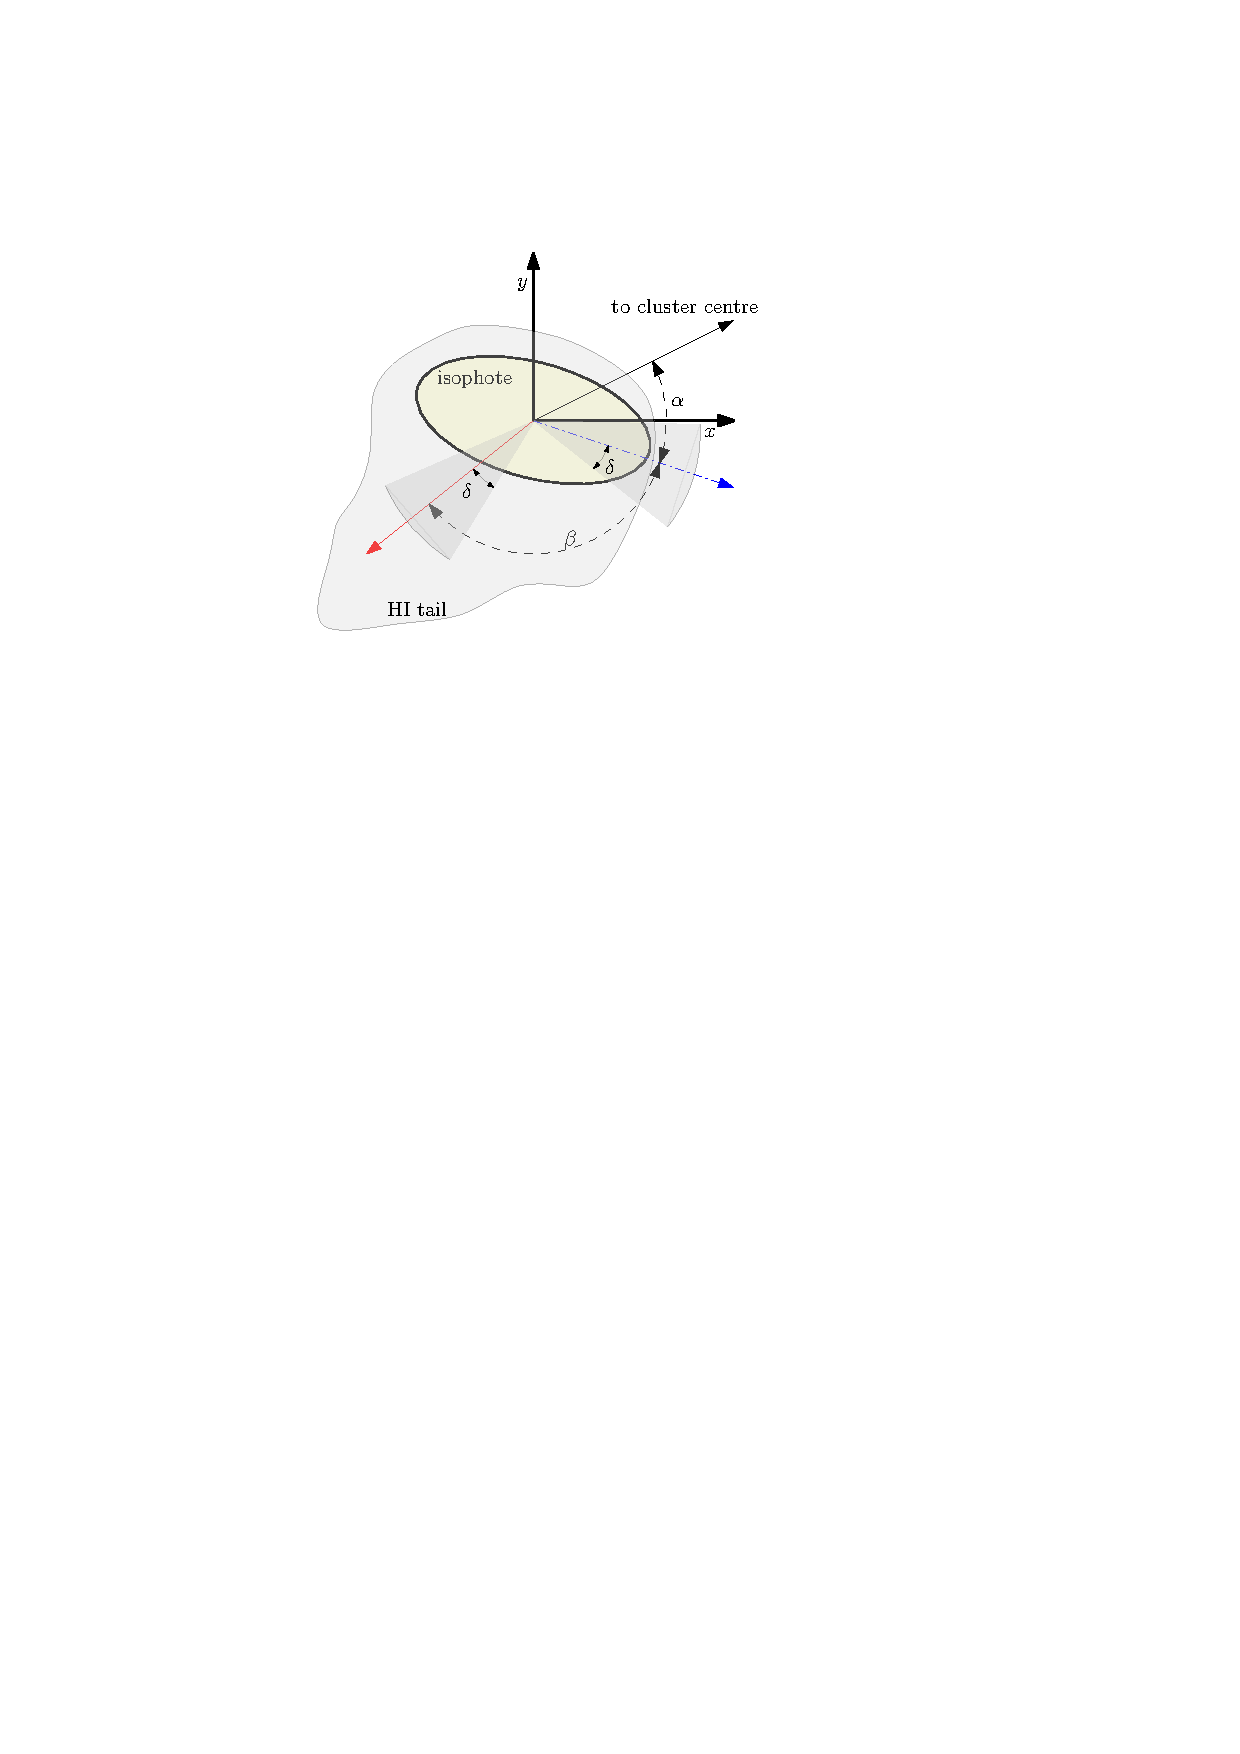
\includegraphics[width=0.65\columnwidth]{alpha_beta_coloured_for_fig.pdf}
\caption{Angles $\alpha, \beta$ definitions used to set up the  requirements for the morphological search. $\delta$ is the angle tolerance used for the selection. Blue and red arrows are defined as in Figure \ref{fig:sb_arrows}. Darker grey shaded regions are the allowed directions of the oriented snapshots tidal stellar tail and \Hi{} tail.}
\label{fig:angles_scheme}
\end{figure}
\begin{figure}
\centering
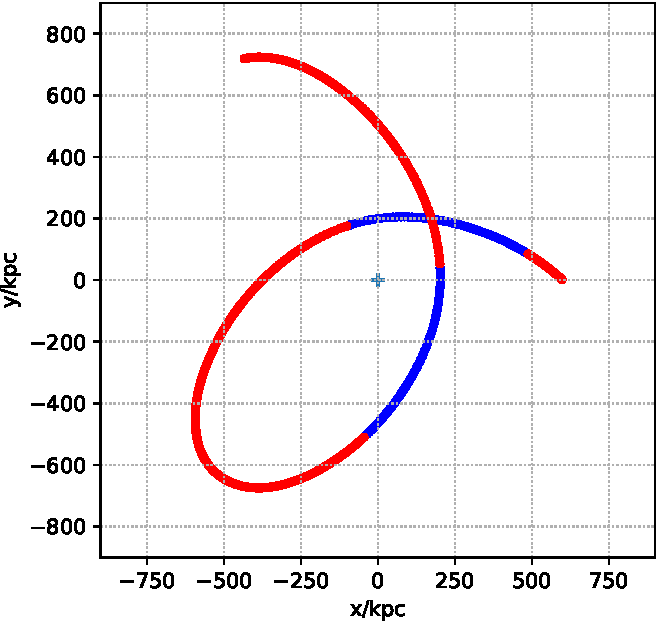
\includegraphics[width=0.55\columnwidth]{good_traj.pdf}
\caption{A trajectory with pericenter of 200~kpc. In blue the orbital phases for which there are snapshots with projected distance and recessional velocity compatible with the ones of NGC~1427A (i.e. snapshots fulfilling requirements (i)-(ii)) for some points of view.
In this case $r_p = 137$~kpc, $v_p = -693$~km/s.}
\label{fig:good_traj}
\end{figure}
We highlight that the search has been carried out using only morphological and orbital parameters, given our focus on the peculiar morphology of NGC~1427A.
Moreover, the criteria used to compare simulations to observations are the ones that best represent the effects of the cluster environment: the relative directions of the tidal pull and the ram pressure stripping. Indeed, the first two requirements put constraints on the orbital position and hence on the orbital phase of the simulated dwarf. The latter two require that the isophotal tail and the neutral gas tail are oriented as in NGC~1427A.
By selecting a faint isophote for criterion (iii) we are tracing the outer tidal extensions of the stellar body.
Inspection of the evolution of the direction of the principal axes of the stellar density distribution along a simulated dwarf galaxy's orbit shows that the galaxy outskirts rapidly forget their initial spatial orientation and become strongly aligned with the cluster center around pericenter and apocenter. On the inward or outbound legs of a galaxy's orbit, this elongation occurs parallel with its orbital velocity. This evidence for a tight correlation between a dwarf galaxy's elongation and its orbital phase, led us to include criterion (iii).

From VST images of \citet[][]{Lee-Waddell2018} \citep[originally from the deep survey presented in][]{Iodice2016} we used the position angle of 15~deg of the fitted ellipse in its Figure 2.
From the \Hi{} maps of Figures 1 and 3 of the same paper (see Figures \ref{fig:hi_contours} and \ref{fig:hi_kin} above) we assumed an inclination of the \Hi{} tail of -135~deg (pointing south-east).
%, see Figure \ref{fig:arrows}.
Given that the direction of the cluster center is around 30~deg north-west, the resulting target angles are $\bar \alpha = 45$~deg, $\bar \beta = 120$ deg, as in Figure~\ref{fig:angles_scheme}.

For each snapshot, we started by finding the orbital phase which fulfils the first two requirements.
Each requirement is satisfied by the set of points of view constituting the generatrices of a cone centered on the galaxy position.
By intersecting two cones it is possible to find the points of view satisfying the requirements.
This is equivalent to solving a quadratic equation (see Section \ref{sec:cone_intersection}) whose two solutions are two points of view satisfying the requirements (i) and (ii).
Each snapshot is then rotated as if it was observed from the peculiar point of view yielding the imposed clustercentric distance and the recessional velocity.
The more radial the orbit is, the higher the number of suitable snapshots which will be further selected using requirements (iii) and (iv), see Figure \ref{fig:good_traj}.

With the assumed cluster center at a distance of 20~Mpc from us (see Section \ref{sec:observations}), we imposed as targets the two quantities $\bar r_p=137$~kpc and $\bar v_p=-693$~km/s with measures for NGC 1427A (the projected distance on the sky and recessional velocity of NGC~1427A relative to NGC~1399).
In order to take into account uncertainties in the measured $\bar r_p$ and $\bar v_p$ and to capture the sensitivity of the procedure to the selected projected distance and recessional velocity, we repeated the same procedure for each simulated snapshot but allowing for other slightly offset targets $r_p$ an $v_p$.
Practically, we fixed an offset in both quantities $r_p = \bar r_p \pm \Delta r$, $v_p = \bar v_p \pm \Delta v$ with $\Delta r = 100$ kpc, $\Delta v = 60$ km/s.
Also we added four other targets: $(\bar r_p \pm \Delta r, \bar v_p)$ and $(\bar r_p, \bar v_p \pm \Delta v)$ with same ($\Delta r, \Delta v$) as before.
Including the exact target $\bar r_p, \bar v_p$, at the end, we had nine targets to check for each snapshot.
In total, we obtained a dataset of 424,656 oriented snapshots.

For each snapshot surviving the selection of requirements (i) and (ii) and oriented so that $r_p$ and $v_p$ are the ones imposed, we created the surface brightness map and \Hi{} map.
We first fitted an ellipse to the contour corresponding to the $26.5$~mag/arcsec$^2$ isophote in $r'$ band.
We computed the second order moments of the \Hi{} map to obtain the direction of the neutral hydrogen tail.
Since we are interested in snapshots with an elongated \Hi{} tail in the South-East direction, we further selected only oriented snapshots with galactic projected velocity on the plane of the sky having a positive projection on the cluster center direction. This removes false positives with a \Hi{} tail inclined with the proper angle but extending towards the cluster center (from the image moments only the direction is returned, not the sense of elongation of the tail).
At the end of this pre-selection, we ended up with 59,896 oriented snapshots.

We then used requirements (iii) and (iv) to further refine the search.
In the following section we shall determine the distribution of the snapshots with tails similar to the observed galaxy using angles $\alpha$ and $\beta$, described above, and a tolerance $\delta$:
\begin{equation*}
\bar \alpha - \delta < \alpha < \bar \alpha + \delta, \qquad
\bar \beta - \delta < \beta < \bar \beta + \delta
\end{equation*}
The selection tolerance $\delta$ is then our main knob to filter-out snapshots oriented as NGC~1427A with angles $\bar \alpha$ and $\bar \beta$. The dependence of the results (and the number of oriented snapshots surviving the selection criteria (i-iv)) on its choice is quite strong, so in all the following histograms we highlight the $\delta$ chosen.


\subsection{Finding points of view - cones intersection}
\label{sec:cone_intersection}
Finding the point of views from which the galaxy appears as having the target projected clustercentric distance ($r_p$) and the proper line-of-sight velocity ($v_p$) is equivalent to solving the problem of intersecting two cones.

Given $\vec x$ the unit vector representing the direction of the point of view, and $\vec r$ and $\vec v$ the clustercentric position and velocity of the galaxy respectively, we can write the following conditions:

\begin{equation}
\label{eq:system}
\begin{cases}
\vec x \cdot \vec v = v_p\\
\vec x \cdot \vec r = \pm R\\
|\vec x|^2 = 1
\end{cases}
\end{equation}
where $R = \sqrt{r^2 -r_p^2}$. By using [$\vec r, \vec v, \vec r \times \vec v$] as basis (right-handed but not orthogonal), it is possible to express $\vec x$ as:
\begin{equation}
    \vec x = a \vec v + b \vec r + c ( \vec r \times \vec v).
\end{equation}
Substituting into \eqref{eq:system}:
\begin{equation}
\begin{cases}
a v^2 + b (\vec r \cdot \vec v) = v_p\\
a(\vec r \cdot \vec v) + b r^2 = \pm R\\
|\vec x|^2 = 1 = a v^2 + b r^2 + c^2 | \vec r \times \vec v|^2 + 2 ab(\vec r \cdot \vec v)
\end{cases}
\end{equation}
The last quadratic equation yields immediately two values of $c$ ($c_1$, $c_2$).

For each chosen sign of $R$, the system yields two solutions: ($\vec x_1$, $\vec x_2$) which can be used to rotate the galaxy snapshot as if it was seen from the directions $\vec x_1$ and  $\vec x_2$.

Each direction can be defined using two angles ($\varphi$ and $\theta$) representing the spherical coordinates of the unit vectors $\vec x_1$ and $\vec x_2$.

\begin{figure}
  \centering
  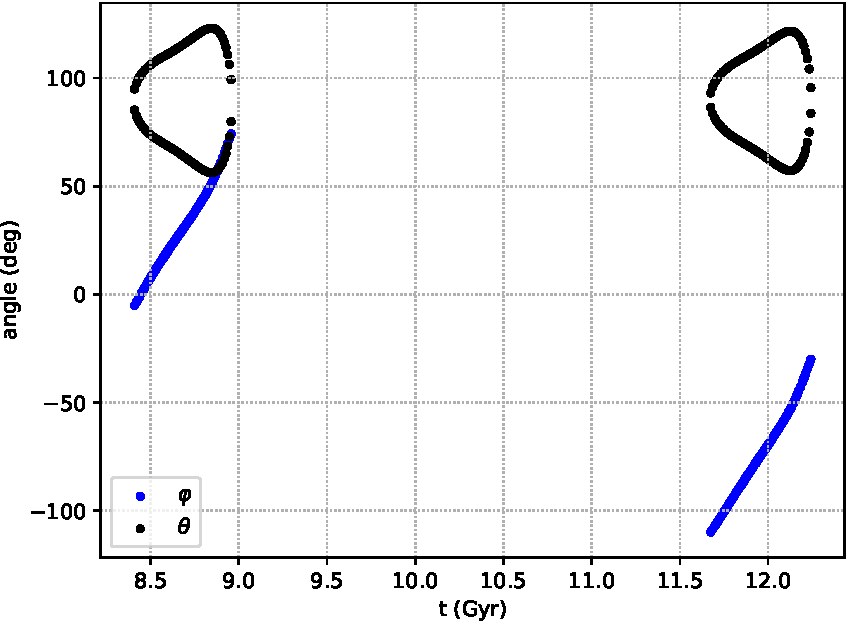
\includegraphics[width=0.8\columnwidth]{angles.pdf}
  \caption{Angles $\varphi, \theta$ defining the points of view of each snapshot of the trajectory of Figure \ref{fig:good_traj}. The angles are used to rotate the selected snapshots in order to obtain the target $r_p, v_p$. Only a subset of snapshots can be oriented to fulfil the requirements.}
  \label{fig:phitheta}
\end{figure}
In Figure \ref{fig:phitheta} an example of rotation angles for a particular simulated orbit is shown.
The angles $\varphi$ and $\theta$ are used to rotate the simulated galaxy as if it was observed from the peculiar point of view yielding the imposed clustercentric distance $r_p$ and the recessional velocity $v_p$.


\subsection{Distribution along the orbit of points of view satisfying the requirements}
\begin{figure}
\centering
\includegraphics[width=0.8\columnwidth]{rps-crop.png}
\caption{The strength of the ram pressure ($\rho v^2$) as a function of normalised time $\tau$ (\cf{} equation \eqref{eq:tau}) for the ID 69 simulations on multiple orbits (orbit pericenter in kpc is indicated in the legend). The colour scales traces orbital distance with respect to the cluster center.}
\label{fig:r_rps}
\end{figure}
We computed the distribution of selected oriented snapshots with respect to the time from the pericenter passage.
We noted that all the snapshots surviving the selection are found within 200 Myr of a pericenter passage.

We ascertain the robustness of this result by varying the tolerance~$\delta$ of the comparison of the angles $\alpha, \beta$ with the observed ones.
Our orbital and morphological criteria are preferentially met by simulations with a stellar mass above $ \approx10^8 $ \Msun{}.
Less massive galaxies and galaxies on radial orbits are completely stripped from their HI gas, see Figure \ref{fig:m_hi}, because of the steep increase of ram pressure around pericenter as shown in Figure \ref{fig:r_rps}.
\begin{figure}
\centering
\includegraphics[width=\textwidth]{m_hi-crop.png}
\caption{Neutral gas mass as a function of normalised time $\tau$ as defined in equation \eqref{eq:tau}.
Each panel is labelled with the simulation ID (cf. Table~\ref{tbl:sim}) and contains information for the simulated dwarf launched on orbits with different pericenter distances (50, 100, 150, 200, 300 kpc identified by the colour legend in the top-left panel).
Gas is compressed when the isolated galaxy enters the cluster and as a consequence it cools down, thus increasing the neutral hydrogen mass.
Obviously, around pericenter, ram pressure stripping is effective at driving down the gas mass (as shown also in Figure~\ref{fig:r_rps}).
}
\label{fig:m_hi}
\end{figure}
Especially for radial orbits, no oriented snapshot is found on orbits of 50 and 100 kpc after first pericenter passage, regardless of the tolerance~$\delta$ considered, as shown in Figure~\ref{fig:histo_peri}.
For the most circular orbits, only snapshots undergoing second pericenter passage survive the selection. This is likely due to the first passage acting as `preprocessing' and making the galaxy potential shallow with higher chances to create tidal tails.
% \todo{I'm currently having a look at the distribution of ellipticity of the fitted isophotes to see how circular, and hence not so tidal, they are. Update: See figure noperi_all_stacked-crop.png }
In Figure~\ref{fig:histo_noperi} we performed the same analysis cumulatively counting all the oriented snapshots (without pericenter distance distinction) but using different isophotes.
The diagrams, even if noisier when using fainter isophotes, convey the same message: there is an abundance of correctly oriented snapshots (with tails as NGC~1427A) around first pericenter passage.
Indeed, tidal tails as those shown in Figure~\ref{fig:panel}, are present in low surface brightness regions of the dwarf, even if they are more difficult to measure.
The counterpart in NGC~1427A would be the faint stellar South-West elongation visible especially in $r'$-band, see Figure~\ref{fig:r_band}.

\begin{figure}
\centering
\includegraphics[width=\textwidth]{histo/histo_iso26.5_bins0.35-16.pdf}
\caption{Histograms of oriented snapshots fulfilling the requirements (i)-(iv), selected to be around first (blue) or second (orange) pericenter and grouped by orbital pericenter distances (50, 100, 150, 200, 300 kpc).
The isophote used to compute the stellar tail inclination is $26.5$~mag/arcsec$^2$ in $r'$ band.
The distribution is peaked at around 150 Myr before pericenter passage, especially in more radial orbits. The result is robust enough to be visible on stricter angle tolerances $\delta = [20, 15, 10]$~deg.
}
\label{fig:histo_peri}
\end{figure}

\begin{figure}
\centering
\includegraphics[width=\textwidth]{histo/iso_comparison_tol15_asym0.0_bins0.35-16.pdf}
\caption{Distribution in time relative to pericenter passage of oriented snapshots fulfilling the requirements (i)-(iv) with tolerance $\delta=15$ deg.
Histograms of selected snapshots are coloured relative to their orbital phase: around first (blue) or second (orange) pericenter.
Each column corresponds to a different isophote used to compute the stellar tidal orientation.
Irrespective of the isophote, the distribution remains peaked  around 150 Myr before pericenter passage.}
\label{fig:histo_noperi}
\end{figure}

\subsection{3D position of the galaxy in the Fornax context}

Based on the above described model, we can produce a quantitative estimation of the galaxy projected radial distance. This measure is actually a testable prediction with distance observations.
Unfortunately, current uncertainties on the distance measurements do not allow to unequivocally assess the position of the galaxy to be in front or behind the cluster center \citep{Georgiev2006}.

Using our models we can see which is the most likely radial distance relative to the cluster center of a galaxy with morphological features like NGC~1427A.
As shown in Figure \ref{fig:distance_prediction}, the preferred line of sight distance is around 200~kpc in front of the cluster center.

It is also possible to compute the flight angle $\gamma$ of the galaxy with respect to the line of sight direction (see Figure \ref{fig:gamma}).
As shown in Figure \ref{fig:velocity_prediction}, from the above models, the most frequent is $\gamma\approx 50$~deg.
Given that the stripped gaseous tail approximately follows the opposite direction of flight, measuring the flight angle in simulations can be useful to assess the real length of the gaseous tail in observations.
Our result would indicate the real tail to be roughly a factor 1.3 longer than the projected one.

\begin{figure}
\centering
\includegraphics[width=0.8\columnwidth]{histo/multi_tol_dist_gauss_bins600_25.pdf}
\caption{Distribution of selected oriented snapshots with multiple tolerance $\delta$ along the projected line of sight. The zero point is 20~Mpc, assumed distance of NGC~1399. Positive values mean the galaxy being \emph{in front of} the cluster center.
%Overplotted a Kernel Desity Estimation for the distribution.
}
\label{fig:distance_prediction}
\end{figure}

\begin{figure}
\centering
\includegraphics[width=0.8\columnwidth]{histo/multi_tol_vel_angle_bins_gauss90_25.pdf}
\caption{Distribution of the flight angle $\gamma$ of selected oriented snapshots with multiple tolerances $\delta$. $\gamma$ is defined as the angle between the galactic velocity vector in the the cluster reference frame and the line of sight direction.
%Overplotted a Kernel Desity Estimation for the distribution.
}
\label{fig:velocity_prediction}
\end{figure}
\begin{figure}
\centering
\includegraphics[width=0.5\columnwidth]{gamma.pdf}
\caption{Definitions of angle of flight $\gamma$ and radial distance $z$. $\vec v$ is the orbital velocity of the galaxy.
}
\label{fig:gamma}
\end{figure}

\section{Discussion} \label{sec:discussion}

\subsection{The asymmetric stellar tidal tails}

\subsubsection{Including asymmetry as a constraint}
As a way of quantifying the asymmetric stellar tides, we computed the non-parametric measure Asymmetry \citep[as defined by][]{Lotz2004} of our oriented snapshots. For each oriented snapshot we fed its surface brightness map to \verb|statmorph| \citep{Rodriguez-Gomez2019} isolating the region of the map within $27$~mag/arcsec$^2$.
As a reference, \citet{Su2021} find an Asymmetry of $0.23$ for NGC~1427A.
We tried to add the Asymmetry to the constraints described in Section \ref{sec:morphological_quest}. Given that almost all the oriented snapshots have an Asymmetry higher than $0.2$ \citep[in line with the average of $0.53\pm0.22$ for galaxies with intense star formation as reported by][]{Conselice2003}, we find that isolating snapshots at least as asymmetric as NGC~1427A do not affect the results.

By plotting Asymmetry on selected snapshots as a function of time from pericenter, as shown in Figure \ref{fig:histo2d_asym}, it can be seen that selected snapshots closer to the pericenter become more symmetric.
A possible reason of this can be hypothesised in the tidal pull close to the pericenter which squeezes the galaxy elongating it, hence removing asymmetric regions of the galaxies.
Indeed all simulations show an Asymmetry greater than the one of NGC~1427A. We note that this is in line with \citet{Rodriguez-Gomez2019} who find a systematically higher asymmetry for simulated galaxy of Illustris and Illustris~TNG \citep{Vogelsberger2014, Pillepich2018}, especially in the low mass range.
In fact, in a numerical simulation each star particle created represents stars of $\approx 1000$ \Msun{}: a simulated galaxy is always more ``granular" than an observed real galaxy due to the limited resolution.

\begin{figure*}
\centering
\includegraphics[width=\textwidth]{histo/hist2d_tp_A_bins20_kde-crop.png}
\caption{2D histogram of selected oriented snapshots with tolerance $\delta=20$~deg.
The distribution is plotted with time from first pericenter passage on the $x$ axis, whereas on the $y$ axis the \emph{Asymmetry} non-parametric measure as defined by \citet{Lotz2004}.
Each column corresponds to a different isophote used to compute the stellar tidal orientation.
We overplot a kernel density estimation of the distribution for the snapshots approaching pericenter. The dotted red line corresponds to the measured \emph{Asymmetry} for NGC~1427A.}
\label{fig:histo2d_asym}
\end{figure*}


% \subsubsection{Including isophotal twisting as a constraint}

\subsubsection{The origin of the asymmetric stellar tidal tails}
\begin{sidewaysfigure}
\centering
\includegraphics[width=0.95\textwidth]{panel68p100-crop.png}
\caption{Evolution in time of the simulation with ID 68 around first pericenter passage, projected in a way that the first column has $r_p = 137$~kpc, $v_p = 693$~km/s, the target values for NGC~1427A.
All the other snapshots are seen from the same point of view as the first one.
Black arrow indicates the direction to the cluster center whereas the green indicates the instantaneous velocity direction of the galaxy projected on the plane of the sky. In the first column, an ellipse fitted on the $26.5$ mag/arcsec$^2$ is shown to highlight the direction of the tidal elongation.
The first row represents the surface brightness of snapshots around the first pericenter. \Hi{} Contours are [$10^{17}, 10^{18}, 10^{19}, 10^{20}, 10^{21}$]~amu~cm$^{-2}$.
Second row the $g'$-$r'$ colour.
Third and fourth row the v-band SPH-average age and velocity of star particles along the line of sight.}
\label{fig:panel}
\end{sidewaysfigure}

An interesting effect of the pericenter passage is the formation of an asymmetric tidal tail, a stellar elongation more pronounced in just one direction, as that shown in the fourth column of Figure~\ref{fig:panel}.
This effect can be investigated by looking at different simulation snapshots evolving with time around a pericenter passage.
We focus our discussion to the case of the galaxy with ID 68 on an orbit with pericenter $100$~kpc.
In Figure~\ref{fig:panel}, the snapshot in the first column is the one who has passed the filters described in Section~\ref{sec:morphological_quest} and represents a snapshot which is in good agreement to the observation, given its stellar and gaseous tail directions and the projected clustercentric distance and recessional velocity.

We can then reconstruct a series of events leading to the generation of the leading edge stellar tail.
The tidal forces exerted by the Fornax Cluster become markedly asymmetric as a galaxy approaches pericenter on a radial orbit.
The steeply deepening gravitational potential well can raise a stronger leading stellar tidal tail while producing a weaker trailing tail during a fast swing-by of a galaxy close to the cluster center.
After pericenter, the leading tail twists due to the curvature of the galaxy's orbit, the rapidly changing direction of the gravitational force, and the internal rotation of the galaxy.
Effectively the pericenter passage injects energy into the galaxy resulting in a temporary increase of its angular momentum (see Section~\ref{sec:kinematics}).

At the same time, the gaseous tail is always directed opposite to the instantaneous velocity.
The result is that the stellar and gaseous tails are very misaligned, almost orthogonal to each other.


\subsection{Possible origin of the Northern Clump in NGC 1427A} \label{NC1427A}
The galaxy NGC~1427A contains a so called Northern Clump (NC), which has been investigated in detail by some authors \citep{Cellone1997, Hilker1997}.
The NC is a clump of blue and very young stars with associated H$\alpha$ emission \citep{Sivanandam2014}.
Even on ground-based images, the NC appears to be composed of two sub-clusters, one to the north of the other.
This impression is strengthened by the HST image presented in Figure \ref{fig:NGC1427A}. The centers of the two sub-clusters are separated by 7'', corresponding to just under 700~parsec.
The NC lies on NGC~1427A's projected rotation axis and hence its line-of-sight velocity agrees very well with NGC~1427A's mean recession velocity \citep{Bureau1996,Chaname2000}. This does not hint at an external origin for this object.
The NC appears to be connected to the north-west rim of the galaxy's main body by a tenuous stream of stars, suggesting it to be displaced along this stream away from the galaxy's main body in a direction that is almost parallel to the major axis of the faint outer isophotes.
If, as in our interpretation of the data, these outer isophotes trace the two diametrically opposite stellar tides raised by the Fornax Cluster forces then this would argue for a purely internal origin of the NC.
It could be a star-formation region (of which there are many inside NGC~1427A) that is being pulled out by the Fornax Cluster tidal forces, leaving behind a stream of stars.
As shown in Figure \ref{fig:panel}, star formation flares up in our simulated dwarf galaxies around pericenter passage and leads to the appearance of scattered bright, blue clumps of active star formation.
These clumps orbit along with the general rotation of their host galaxy.
The spatial location and the time of appearance of these clumps are erratic and differ between galaxies and between orbits.
For instance, a star-forming clump is first visible to the top-right of the galaxy in the snapshots 108~Myr before pericenter passage (second column in Figure \ref{fig:panel});
it rotates clockwise, and disappears again after the 137~Myr past pericenter passage snapshot.
Likewise, other clumps with similar lifespans pop in and out of existence around pericenter passage.

Based on these simulations and the available observational data, we suggest that the NC is precisely such a star-forming clump. This interpretation is consistent with its very young age and blue colour, its presence around the time that NGC 1427A is expected to be near pericenter passage (this is required to explain all other characteristics of NGC 1427A), and its kinematics being in line with the galaxy's global velocity field.

%In simulations, as shown in Figure \ref{fig:panel}, around pericenter passage, star formation moves from the galactic center to the gas-rich tail because of ram pressure.
%Many clumps of young stars are therefore formed, suggesting a formation scenario for the Northern Object.
%After pericenter, the galaxy relaxes and stars are being formed again in the galaxy core.

\section{Conclusions}
We carried out a set of simulations of gas-rich late-type dwarf galaxies in a Fornax-like cluster environment.
We isolated snapshots with morphological properties similar to the peculiar galaxy NGC~1427A. The properties have been chosen to be representing the impact of the environment on the dwarf.
We found that the main effects generating peculiar morphology are indeed the combination of ram pressure and tidal interaction close to the cluster center and galaxy rotation.
We saw that the most likely scenario which recreates NGC 1427A tails morphology is assuming the galaxy to be on a very radial orbit with its tail almost aligned with the line of sight, pointing towards the observer.
This naturally leads to a gas kinematic configuration consistent with \Hi{} observations: in the westward part, gas attached to the stellar body of the galaxy is receding whereas the eastward part is stripped and dragged towards the observed by the intra-cluster medium (or ICM), therefore having a smaller recessional velocity, see Figures \ref{fig:sim_hi_kin} and \ref{fig:hi_kin}.

From the analysis of the morphology of the simulated snapshots motivated by environmental effects, we found an excess of snapshots revealing similar NGC~1427A structure around 150 Myr before pericenter passage.
It should be highlighted that this result comes from a suite of simulation which has not been tailored from the beginning to reproduce NGC~1427A.
Nonetheless, interestingly, falsifiable predictions on the location and orbital phase of the galaxy can be made.

We can sum up the main results in the following points:
\begin{itemize}
    \item Perpendicular gaseous and stellar tails are explainable given that they are subject to different environmental effects.
    \item Tails geometry is crucial to unravelling the direction of motion of the galaxy and its orbit.
    \item From our suite of simulation it is evident how around \textasciitilde 150~Myr before first pericenter passage, a morphological tail structure like the one of NGC~1427A emerges in galaxy falling into a Fornax-like cluster.
    \item In simulations, around pericenter, clumps of newly formed stars can form. This is coherent with a formation scenario of NGC~1427A's Northern Clump as a star formation region pulled out by tidal forces.
    \item Following our modelling it is possible to estimate the most likely position of a NGC~1427A-like galaxy to be around 200 kpc in front of the cluster center. Also, the most likely flight direction (represented by the angle $\gamma$ in the paper) is around 50~deg.
\end{itemize}

\section*{Data availability}
The data underlying this article and the algorithms used are available at this GitHub repository: \url{https://github.com/elehcim/ngc1427apaper}.\\
A publicly available \texttt{python} package to analyze the simulations in this dataset can be found at this GitHub repository: \url{https://github.com/elehcim/simulation}.

% !TEX root = thesis.tex
{
\cleardoublepage% Move to first page of new chapter
\let\cleardoublepage\relax% Don't allow page break
\noindent \small{Based on: \emph{Probabilistic modelling of general noisy multi-manifold data sets}, Canducci~M., Ti\v{n}o~P., Mastropietro~M. Submitted to \emph{Artificial Intelligence} \citet{Canducci2021}.
Part of this work has been carried out during the planned SUNDIAL secondment at the Computer Science Department of the University of Birmingham.
}
\chapter{Low-dimensional manifolds}
\label{ch:manifolds}
}

\abstract{
The intrinsic nature of noisy and complex data sets is often concealed in low-dimensional structures embedded in a higher dimensional space.
%Number of methodologies have been developed to extract and represent such structures in the form of manifolds (i.e. geometric structures that locally resemble continuously deformable intervals of $\mathbb{R}^j$ \footnote{$j$ is the manifold dimensionality.
%Mathematically, continuous deformation corresponds to homehomorphism: one-to-one continuous mapping with continuous inverse.}).
% Usually a-priori knowledge of the manifold's intrinsic dimensionality is required.
% Additionally, their performance can often be hampered by the presence of a significant high-dimensional noise aligned along the low-dimensional core manifold.
In real-world applications, the data can contain several low-dimensional structures of different dimensionalities.
We propose a framework for dimensionality estimation and reconstruction of multiple noisy manifolds embedded in a noisy environment.
%To the best of our knowledge, this work represents the first attempt at detection and modelling
%of a set of coexisting general noisy manifolds by uniting two aspects of multi-manifold learning:
%the recovery and approximation of core noiseless manifolds and the construction of their probabilistic models.
%The easy-to-understand hyper-parameters can be manipulated to obtain an emerging picture of the multi-manifold structure of the data.
% We demonstrate the workings of the framework on two synthetic data sets, presenting challenging features for state-of-the-art techniques in Multi-Manifold learning.
% The first data set consists of multiple sampled noisy manifolds of different intrinsic dimensionalities, such as M\"{o}bius strip, toroid and spiral arm. The second one is a topologically complex set of three interlocked toroids.
% Given the absence of such unified methodologies in the literature, the comparison with existing techniques is organized along the two separate aspects of our approach mentioned above, namely manifold approximation and probabilistic modelling.
The framework is then applied to a complex data set containing simulated gas volume particles from a particle simulation of a dwarf galaxy interacting with its host galaxy cluster.
Detailed analysis of the recovered \mbox{1-D} and 2-D manifolds can help us to understand the distribution of various physical quantities in such complex systems.
The technique allows to isolate the evolution of quantities around tails of a simulated jellyfish galaxy, so that of star formation regions and the mixing of galaxy gas and cluster gas can be studied.
}
\section{Introduction}


Dimensionality reduction and Density Estimation of raw data, are commonly used tools to extract information from complex and noisy data sets.
Due to dependencies among measured attributes of real world data,
the data is often distributed along low-dimensional structures in a higher dimensional measurement space.
This realisation has driven the development of a variety of Manifold Learning algorithms.
Principal Component Analysis \citep[PCA, ][]{Pearson1901} is a well understood and widely used linear dimensionality reduction scheme.
%\Marco{It can be considered the progenitor of Manifold Learning, where the data is assumed to lie on a multivariate Gaussian and the recovered principal components capture the variance of the data along orthogonal directions.}
However, by design, PCA cannot appropriately capture non-linear low-dimensional structures.
% This lack of flexibility has been addressed by non-linear dimensionality reduction algorithms such as Isomap \cite{Tenenbaum2319}
% and Locally Linear Embedding \citep[LLE][]{Roweis00nonlineardimensionality},
% where the manifold is approximated by a neighbourhood graph and a neighbouring preserving map respectively.
% Both methods take advantage of the definition of a manifold as a locally linear low dimensional structure of dimension $j$.

% Many other Manifold Learning algorithms aiming to provide suitable approximations to low-dimensional data manifold have been proposed.
% Examples include Laplacian eigenmaps \citep{Belkin01laplacianeigenmaps},
% Hessian eigenmaps \citep{Donoho5591},
% Local Space Tangent Alignment \citep[LSTA, ][]{Zhang02principalmanifolds},
% C-Isomap \citep[an extension of Isomap to conformal embeddings][]{Silva:2002:GVL:2968618.2968708},
% NMDS \citep[non-metric formulation of Multidimensional Scaling (MDS)][]{doi:10.1002/bs.3830040308, Cox2008, Kruskal1964},
% Riemannian Manifold Learning \citep[RML, ][]{10.1109/TPAMI.2007.70735}.

% In \cite{boissonnat:hal-01615863} (and bibliographic references therein) a different angle, based on computational geometry,
% has been proposed in order to extract low-dimensional manifolds from data samples.
% Here, simplicial complexes (such as Delaunay triangulations, $\alpha$-complexes and filtrations)
% are used for manifold reconstruction.
% With these techniques it is possible to infer geometrical and topological properties of data points
% that uniformly sample a single manifold embedded in a higher dimensional space.

% While such techniques are potentially powerful and theoretically well grounded,
% their capability to naturally handle high-dimensional noise aligned along low-dimensional manifolds is limited.
% Besides the sensitivity to the noise issues, it is often required that the intrinsic data dimensionality is known a priori.

Generative Topographic Mapping \cite[GTM, ][]{Bishop1998GTMTG} was proposed as a probabilistic formulation of the Self-Organizing Map \citep{Kohonen1982}.
Its main advantage is that instead of treating noisy manifold as a core low-dimensional manifold to be discovered,
plus some ``noise" around it that somehow needs to be dealt with,
it formulates a consistent manifold-aligned density model in the form of a constrained mixture of Gaussians.
The location parameters (means) of the Gaussian components are constrained to lie on a smooth manifold
-- most commonly a smooth image in the data space of a two-dimensional interval (latent space).
%The original GTM formulation is trained in the maximum likelihood framework using the the Expectation-Maximization (E-M) algorithm \citep{10.2307/2984875}.
%Because of the sensitivity to initialization, a suitable initialization is required (e.g, using PCA).
% Bayesian formulations of GTM have also been proposed \cite{Olier2008VariationalBG}.

%Other global density estimators, whether non-parametric, e.g. Parzen windows \cite{parzen1962estimation}
%(and its extensions such as Manifold Parzen Windows \cite{NIPS2002_2203}, Fast-Parzen Windows \cite{5178637}),
%or semi-parametric, e.g. Infinite Gaussian Mixture model\cite{10.5555/3009657.3009736},
%are not designed to extract a representation of the embedded low-dimensional structures.
%They also may be computationally expensive to train and/or evaluate.

% To deal with complex data sets, where several manifolds of different dimensionalities can co-exist,
% generalizations of the previous methods have been developed:
% Multi-Manifold Discriminant Analysis (MMDA, \cite{Yang:2011:MDA:1963661.1963809}),
% Sparse-Manifold Clustering and Embedding (SMCE,\cite{NIPS2011_4246}),
% Multi-Manifold Isomap (M-ISOMAP\cite{Fan2012IsometricML}),
% Multi-manifold Proximity Embedding  (MPE,\cite{Fan:2016:EIM:2903049.2903101}),
% Multi-Manifold LLE (MM-LLE,\cite{Hettiarachchi:2015:MLL:2791619.2792198}),
% S-Isomap++ \cite{2017arXiv171006462M},
% Hierarchical GTM \cite{Tino_PAMI_2002}.
% However, based on the same assumptions as their predecessors, the methods still need to be informed
% about the dimensionalities of the different manifolds
% and struggle when dealing with topologically complex, noisy structures}.

In \citet{Canducci2021} we propose a framework for automated dimensionality estimation and reconstruction
of multiple noisy manifolds embedded in a noisy environment called \emph{Abstract Generative Topographic Mapping} (AGTM).
%\begin{itemize}
%  \item it proposes a new robust dimensionality index estimation for data points,
%  \item through a dedicated manifold crawling mechanism it allows for completely abstract manifold representations in the GTM latent space (instead of a regular grid), and
%  \item it has Gaussian noise components naturally aligned along the manifold, unlike the spherical noise models in the original GTM and \cite{10.1007/978-3-540-87481-2_37}.
%\end{itemize}
%Manifold aligned noise models in GTM were also considered in \cite{Bishop1998DevelopmentsOT},
%but under the assumption of simple latent space structure in the form of $j$-dimensional interval.
%The key idea was to impose larger and smaller variances in directions locally parallel and perpendicular, respectively, to the manifold.
Since our latent space is a discrete structure (abstract graph representing a skeleton of a given manifold),
we formulate local noise models through kernel based estimates of the local covariance matrix of the data,
with trainable scale parameter to allow for optimized overlapping of the neighbouring Gaussian components.
The work is inspired by \cite{10.1007/978-3-540-87481-2_37}, but extends and generalizes it, so that densities aligned along arbitrary manifolds (even non-orientable ones such as M\"{o}bius strip) can be captured,

The detailed aspects of AGTM will not be described in this thesis, because its treatment is not suitable for this context.
However, after the identification of the low-dimensional manifold as in \citet{Canducci2021}, instead of the probabilistic one, we'll use the SPH approach to estimate densities to compute physical quantities along the manifolds.

%This is achieved by replacing the simple Euclidean latent space (generally parametrized as a discretized interval of $\mathbb{R}^j$)
%with an abstract graph reflecting the topology of the data manifold that, when embedded in the data space,
%provides a manifold skeleton around which the noise models can be organized.

%Our work presents a radical reformulation of GTM to capture and model low-dimensional general noisy manifolds
%through a dedicated abstract graph-structured latent space reflecting the core manifold structure, specific to each noisy manifold.
% \citet{Bacciu13} present another radical generalization of GTM in the reverse direction -
% this time keeping the original simple latent space structure, but allowing for abstract structure in the data space - the space of trees.

%The paper has the following organization: in section \ref{sec:Methodology} we set up the scene,
%explain the broad outline of the methodology and introduce the synthetic data set on which different steps of the methodology will be demonstrated.
%Section \ref{sec:AGTM} introduces the core model of our methodology, Abstract~GTM (AGTM),
%representing density aligned along a single manifold.
%We explain how the abstract latent space graph representing topology of the data manifold is
%extracted through manifold crawling and how this graph is then embedded in the data space along with the suitable set of noise models.
%We also show how to calculate local curvature at the edges of the embedded graph,
%taking advantage of the smooth manifold description provided by AGTM.
%Section \ref{sec:D_Index} defines our notion of dimensionality index for individual points.
%We also offer a computationally efficient alternative to Multi-Manifold Crawling.
%The price to pay for gains in efficiency is weaker detection stability of low dimensional manifold entities buried in the data.
% Section \ref{sec:Comparison} presents an experimental comparison on two synthetic data sets of our methodology
% with alternative multi-manifold learning and probabilistic modelling methods.
%Even though our methodology aims to provide density models of multiple low-dimensional manifolds buried in the data,
%we organise the comparative experiments separately for the multi-manifold capture and probabilistic modelling aspects of our work.
%This is because to the best of our knowledge, no other method exists that can simultaneously recover low dimensional
%representations of an unknown number of manifolds while building their probabilistic models.

%Our main contributions can be summarized as follows:
%\begin{itemize}
%    \item Formulation of a new dimensionality index assigned to individual points based on which point cloud can be partitioned into background points and sets representing cloud points organised along noisy low-dimensional manifold structures;
%    \item Development of a recursive crawling algorithm for the extraction of multiple low-dimensional, noisy manifolds embedded in a higher dimensional space: Multi-Manifold crawling;
%    \item Extension of GTM's applicability to a broad class of manifolds (\eg{} non-orientable or closed manifolds) by reformulating the latent space as an abstract graph and introducing a manifold-aligned noise attached to the embedded nodes of the latent graph: Abstract GTM.
%    The abstract latent space and its embedding allows us to {\em understand the important global structural features of the underlying manifolds}
%%     - an important aspect of our methodology bringing manifold learning under the umbrella of Artificial Intelligence.
%\end{itemize}

The methodology is applied in section \ref{sec:Ex_JellyFish} to a numerical simulation of a dwarf galaxy falling into the gaseous halo of a Fornax-like cluster, a snapshot of the simulation ID 69 described in Chapter~\ref{ch:simulations}.
{The point cloud generated by the simulation presents non linear, noisy, low dimensional structures,
providing for an ideal test bed for our methodology.}
We extract and model two of the most significant manifolds, suggesting a possible scenario for formation of new stars in such a disrupted dwarf galaxy.
% TODO mention the quantities varying along the manifold.

\section{Methodology} \label{sec:Methodology}
We refer to \citet{Canducci2021} for the thorough mathematical presentation of the technique.
Here we sketch the main ideas and we set up the scene in order for the reader to understand the overall methods used.
In the following we give a brief outline of our methodology to robustly detect the manifolds.

\subsection{Diffusion filtering} \label{sec:SAF}
Consider a point cloud
\[\mathcal{Q} =\{\vect{t}_1, \vect{t}_2,...,\vect{t}_L\},\quad \vect{t}_i \in \mathbb{R}^d\]
containing points sampled from an unknown number of noisy lower-dimensional manifolds embedded in a noisy environment (e.g., points generated from a broad $d$-dimensional distribution).
We first apply a physics-based diffusion method, Structure-Aware Filtering Technique \citep[SAF,][]{Wu2018}, that collapses points in close vicinity of dense structures onto them, resulting in a diffused data set:
\[\tilde{\mathcal{Q}} =\{\tilde{\vect{t}}_1, \tilde{\vect{t}}_2,...,\tilde{\vect{t}}_L\},\quad \tilde{\vect{t}}_i \in \mathbb{R}^d.\]
% NOTE how SAF works?
% It defines a velocity as the gradient of the smoothed density (you can use two kernel, one for repusion, one for attraction) and advects points until convergence.
The SAF method moves points towards high density regions, enabling points in the vicinity of a noisy manifold to migrate towards its ``spine" or ``mean surface".

Assuming that the data structures to be modeled are more densely sampled than the noisy environment
we first filter the data sets $\mathcal{Q}$ and $\tilde{\mathcal{Q}}$ by removing point couples $(\vect{t}_i,\tilde{\vect{t}}_i)$ that have sparse neighbourhood in \emph{both} $\mathcal{Q}$ \emph{and} $\tilde{\mathcal{Q}}$.
In particular, around each $\vect{t}_i$ and $\tilde{\vect{t}}_i$ we construct a hyperball $\mathcal{B}(\vect{t}_i;r)$ and $\mathcal{B}(\tilde{\vect{t}}_i;r)$ in $\mathbb{R}^d$ of radius $r>0$.
In case a point $\vect{t}_i$ lies further apart from a manifold, both hyperballs will be sparsely populated.
Hence, if both $\mathcal{B}(\vect{t}_i;r)$ and $\mathcal{B}(\tilde{\vect{t}}_i;r)$ contain less points than a pre-specified threshold $\tau>0$ the points $\vect{t}_i$ and $\tilde{\vect{t}}_i$ are removed from their corresponding data sets.

%\subsection{Manifold analysis overview}
Following this, the first task in capturing the multi-manifold structure in $\tilde{\mathcal{Q}}$ is to estimate local dimensionality of the cloud point around each $\tilde{\vect{t}}_i$
in the form of a \emph{dimensionality index} $\delta_i$ (section \ref{sec:D_Index}).
Using the dimensionality indices, we partition the data into subsets $\tilde{\mathcal{Q}}_j$ according to the local dimensionalities $j=1,2,...,d$.

Since $\mathcal{Q}_j, \tilde{\mathcal{Q}}_j$ can contain several distinct sampled manifolds of dimensionality $j$,
we use a dedicated \emph{manifold crawling} procedure operating on $\tilde{\mathcal{Q}}$ to separate the individual manifolds (section \ref{sec:Crawling}).
Moreover, the crawling also produces for each manifold a graph structure embedded in $\mathbb{R}^d$ representing a piece-wise linear ``skeleton" approximation of the spine of the noisy manifold.
%To isolate a low dimensional manifold and generate the topography of the latent space containing all the information about a detected manifold the \emph{manifold crawling} algorithm has been developed \citep[see section 3.2 of][]{Canducci2021}.


%For every manifold, the associated graph will then function as an abstract latent space of a generalized form of Generative Topographic Mapping (GTM) \cite{Bishop1998GTMTG} that we call \emph{Abstract GTM} (AGTM).
%Using points in $\tilde{\mathcal{Q}}$, the generalized GTM produces manifold aligned density models. %(section \ref{subsec:GTM}).

%Finally, if a single summary model is required, density models of all detected manifolds (AGTMs) can be grouped together in a hierarchical mixture model \cite{Tino_PAMI_2002} representing in a concise manner the global density of the low-dimesional structures in the dataset $\tilde{\mathcal{Q}}$.

\subsection{Dimensionality estimation} \label{sec:D_Index}
Around each $\tilde{\vect{t}}_i \in \tilde{ \mathcal{Q}}$ we perform local Principal Component Analysis (PCA) using points from  $\mathcal{B}(\tilde{\vect{t}}_i;r) \cap \tilde {\mathcal{Q}}$, obtaining eigenspectrum
\[\lambda_{i,1} \ge \lambda_{i,2} \ge ... \ge \lambda_{i,d}.\]

%The dimensionality index of $\tilde{\vect{t}}_i \in \tilde{ \mathcal{Q}}$ used in \cite{10.1007/978-3-540-87481-2_37} (limited to 3-dimensional data) was obtained as
%\begin{equation}
%	\delta^O_i = \argmax_j S_{i,j}
%\end{equation}
%where $ S_{i,1} = {\lambda}_{i,1} - {\lambda}_{i,2}$, $S_{i,2} = 2 ({\lambda}_{i,2} - {\lambda}_{i,3})$ and $S_{i,3} = 3 {\lambda}_{i,3}$.

We suggest a general method for computing dimensionality index of points distributed in spaces of arbitrary finite dimension $d$, based on renormalized eigenvalues,
\[
\tilde{\lambda}_{i,j} = \frac{\lambda_{i,j}}{\sum_{k=1}^d \lambda_{i,k}},
\]
viewed as ``likelihoods" of different dimensionalities $j$ of the cloud of points around $\tilde{\vect{t}}_i$.
\paragraph{Simplex}
Note that
$\tilde{\Lambda}_i = (\tilde{\lambda}_{i,1}, \tilde{\lambda}_{i,2},\dots,\tilde{\lambda}_{i,d})$
lies in the ($d-1$)-dimensional simplex $\mathcal{S}_0$ with vertices:
\begin{align*}
\s_1 &= (1, 0, 0, \dots,0),\\
\s_2 &= (1/2, 1/2, 0, \dots, 0),\\
\s_3 &= (1/3, 1/3, 1/3, \dots, 0),\dots\\
\s_d &= (1/d, 1/d, 1/d, \dots ,1/d).
\end{align*}


%The simplex $\mathcal{S}_0$ is a subset of the standard simplex $\mathcal{S}$ with vertices equal to the standard basis
%\begin{align*}
%\e_1 &= (1, 0, 0, \dots, 0),\\
%\e_2 &= (0, 1, 0, \dots, 0),\\
%&\vdots\\
%\e_d &= (0, 0, 0, \dots, 1).
%\end{align*}
%Considering $\mathcal{S}$ as the simplex of multinomial distributions,
%the appropriate Riemannian geodesic distance is the Fisher distance % FIXME why the Fisher?
%\citep{Lebanon:2005:RGS:1087529}.
It is useful to see $\mathcal{S}_0$ as a subset of the the simplex of multinomial distributions, so that for any point of the simplex, $\tilde{\Lambda}_k \in \mathcal{S_0}$,
we will compute its distance from the vertex $\s_j$ using the Fisher distance \citep{Lebanon:2005:RGS:1087529}:
\begin{equation}
	\label{eq:FishDist}
	d_J(\tilde{\Lambda}_k,\s_j) = 2\arccos{\left(\sum_{i=1}^{d} \sqrt{(\tilde{\lambda}_{ki}\, s_{ji})}\right)}.
\end{equation}
We therefore assign to each point $\tilde{\vect{t}}_i$ of the dataset a
dimensionality index $\delta_i$ as the index of the closer (assuming the $d_J$ distance metric) vertex of the simplex:
%Note that the vertex $\s_j$ of $\mathcal{S}_0$ corresponds to the ideal normalized eigen-spectrum of a $j$-dimensional neighbourhood.
%Hence, we will quantify the degree to which the neighbourhood of $\tilde{\vect{t}}_i$ resembles a $j$-dimensional hyperplane in $\RR^d$ by the closeness of $\tilde{\Lambda}_i$ to $\s_j$
%in terms of the geodesic distance
%\eqref{eq:FishDist},
\begin{equation}\label{eq:idxHard}
	\delta_i = \argmin_j d_J(\tilde{\Lambda}_i,\vect{s}_j).
\end{equation}

In \citet{Canducci2021} also a ``soft" and spatially smoothed version of the dimensionality index is proposed.

\begin{figure}[ht!]
  \includegraphics[width=\textwidth]{Figures_png/Classified_Simplex_lowRes.pdf}
  \caption{Simplex $\mathcal{S}_0$ in three dimensions. p1, p2 and p3 are the analogous of the $\s_1, \s_2, \s_3$ vertexes. The three parts of the simplex are coloured depending on the minimum distance vertex using the Fisher metric \eqref{eq:FishDist}.}
  \label{fig:simplex}
\end{figure}

\subsection{Crawling} \label{sec:Crawling}
%\begin{figure}[th!]
%\begin{subfigure}[t]{\textwidth}
% \includegraphics[width=\textwidth]{Figures_png/RanStrip_Whole.png}
% \caption{}
% \label{subfig:MGraph}
%\end{subfigure}
%\begin{subfigure}[t]{\textwidth}
% \includegraphics[width=\textwidth]{Figures_png/Mobius_Whole.png}
% \caption{}
% \label{fig:Mobius_Whole}
%\end{subfigure}
%%  \subfloat[][]{\label{subfig:MGraph}\includegraphics[width = 0.9\textwidth]{Figures_png/RanStrip_Whole}} \\
%%  \subfloat[][]{\label{subfig:MGraph_Emb}\includegraphics[width = 0.9\textwidth]{Figures_png/Mobius_Whole}}
%\caption{ (a) shows the classic GTM setup;
%the leftmost panel is a representation of the latent space discretized in a grid of points $x_i$.
%The $j$-dimensional interval $[-1,+1]^j$ is mapped through the parametrized function $\vect{y}(\mathcal{X};W)$ onto the data space with a spherical Gaussian centered on each point assumed as noise.
%The noise model aims at describing the true distribution of points in the data space (rightmost panel).\\
%(b) is a sketch of \emph{AGTM}.
%The latent space is substituted with an abstract graph, shown here for the M\"obius strip, together with its topological representation (the two arrows pointing in opposite directions on the shortest edges of the graph).
%Function $f(\cV;\W)$ maps the graph onto the data space and manifold-aligned noise models are estimated on each graph's node $\overline{\vect{v}}_i$ % FIXME why f is not bold?
%The true noisy distribution is displayed in the rightmost panel.}
%\end{figure}


We leave once again the mathematical details to \citet{Canducci2021} for a clear and thorough exposition, and we highlight here the fundamental ideas.
% TODO This crawling is part of a more general technique to extract probabilistic models of filaments/manifolds and smooth the extracted filament by training a maximum likelihood.
%TODO Difference with Disperse. We have instead a Knowledge aware starting point.

After having identified the subsets of points belonging to manifolds of different dimensionalities, for each dimension we would like to isolate the (possibly multiple) embedded manifolds they can contain.
The goal is to create a latent space containing all the information about a detected manifold $\cM$ embedded in a higher dimensional data space.
%If we then define a probability distribution $p(v)$ on the latent-variable space, this will induce a distribution
%$p(\vect{t}|\f)$ in the data space, which is what we are seeking in the end.
%The assumed distribution in the data space is a Gaussian with the local manifold-aligned covariance matrix $\Sigma$ computed as:
%\[...\]

The mapping $\f: \cV \to \RR^d$ from the latent space to the data space is, following \citet{Bishop1998GTMTG},
a nonlinear model, linear in parameters.
The latent space grid structure can be represented by an abstract undirected graph $\cG = (\cV,\cE)$, where each grid point corresponds to a vertex $v_i \in \cV$ and edges $e_{ij} \in \cE$ are connecting vertices corresponding to neighbouring grid points.
In particular, the image of a vertex $v \in \cV$ %under $\Phi = (\phi_1,..., \phi_M)^\top$
is obtained as $\overline{\vect{v}}_i = \f(v)$ operating on the latent space $\cG$ \citep[see section 3.1 of][for details]{Canducci2021}.
The goal of the crawling is to create a manifold skeleton formed by the embedded graph
$\overline{\cG} = (\overline{\cV},\overline{\cE})$.%, where the vertexes
%$\overline{\cV} = \{ \bar{\vect{v}}_i, ..., \bar{\vect{v}}_K\}$ and the edges
%$\overline{e}_{ij} \in \overline{\cE}$. % whenever ${e}_{ij} \in {\cE}$.
%\begin{equation}
%  \overline{\vect{v}}_i = \f(v;\W) = \W \vect{\Phi}(v),
%  \label{eq_f}
%\end{equation}
%where $\mathbf{W}$ is a $d \times M$ matrix of weights and $\vect{\Phi}$ is a set of basis functions $\phi_m: \cV \to \RR$, $m=1,2,...,M$,

\paragraph{Manifold crawling}
Briefly, starting from a randomly selected data point $\ti_0$, a local PCA in $\cB(\tilde{\vect{t}}_0;r)$ is performed and depending on the dimensionality $\delta_j$ of $\ti_0$, the first $j$ largest eigenvectors $\vect{u}_j$ are selected to define the tangent space to the manifold $\cM$.
For each local eigenvector $\vect{u}_j$, a step of length $\eta\, r$ is performed in its directions ($\pm \vect{u}_j$). A new vertex $\bar{\vect{v}}$ of the graph $\bar{\cV}$ is then selected as the closest data point to $\vect{z}_j^{\pm} = \ti_0 \pm \eta\, r\, \vect{u}_j$.
The graph $\bar{\cV}$ is gradually constructed in this way.
%This can be... % FIXME how do I go back to the latent space?

At the end of this step, we obtain: a latent space graph $\cG$, a set of points $\ti_i$ belonging to the manifold, and an embedding $\f: \cV \rightarrow \RR^d$.
This will enable us to naturally represent density models of noisy manifolds of much more intricate structure than that of a smoothly embedded low dimensional interval.
%The abstract latent space graph representing topology of the data manifold is
%extracted through manifold crawling and how this graph is then embedded in the data space along with the suitable set of noise models.

The latent space graph is interesting because it contains information about the topology of the manifold: the local curvature, the local elongation.
From the derivative along the edges $e_{ij}$ of the mapping $\f$ it is possible to compute the local curvature and elongation (see Figure \ref{fig:curvatureJF}).

%This graph is then embedded in the data space along through the embedding $\f$.

%The latent space grid structure can be represented by an abstract undirected graph $\cG = (\cV,\cE)$, where each grid point corresponds to a vertex $v_i \in \cV$ and edges $e_{ij} \in \cE$ are connecting vertices corresponding to neighbouring grid points.
%The structure of $\cG$ is directly reflected in the latent grid shown in Figure \ref{subfig:MGraph_Emb}.

%Through the embedding $\f$, we can compute the images $\bar{\vect{v}}_i=\f(v_i)\in \RR^d$ of the nodes of $\cG$.
%A spherical Gaussian noise model is then positioned at each skeleton node
%$\f(\vect{v}_i)$, thus representing the noisy manifold as a mixture of $K$ Gaussians centered at $\f(\vect{v}_i)$ (see Figure \ref{subfig:MGraph}).

%The manifold skeleton will then be formed by the embedded graph
%$\overline{\cG} = (\overline{\cV},\overline{\cE})$, where
%$\overline{\cV} = \{ \bar{\vect{v}}_i, ..., \bar{\vect{v}}_K\}$ and
%$\overline{e}_{ij} \in \overline{\cE}$ whenever ${e}_{ij} \in {\cE}$.
%Each node $\vect{v} \in \cV$ is located in the data space $\vect{v}=\f(\bar{\vect{v}})$ and constitutes the center of a local Gaussian component.

\section{Experiments on a simulated jellyfish galaxy}\label{sec:Ex_JellyFish}

We will demonstrate our methodology on analysis of formation of a peculiar astronomical object, a simulated ``jellyfish galaxy".
% The term "jellyfish galaxy" refers to an observed galaxy showing signs of gas stripping \cite{Poggianti2017}, whose signatures are a dense "head" of mainly gas and stars and an elongated gaseous, star-forming tail.
% Particularly interesting is the case of jellyfish galaxies originated as dwarf galaxies disrupted by their environment (e.g., a cluster of other galaxies). Dwarf galaxies, due to their low mass, are more susceptible to the environment's interaction than their more massive analogous.
Even though the characteristic feature of these objects is their gaseous tail, little is known about its detailed structure and physical properties, including the rate at which new stars are formed.

Analyzing in detail the SFR of these tails can provide useful insights on the formation scenario of galaxies infalling in a cluster \cite{Ebeling2013}.
As an example, dwarf galaxy NGC~1427A in the Fornax cluster, described in detail in Chapter \ref{ch:ngc1427a} provides an interesting case of still unclear formation scenario.
%It has been observed multiple times, but a generally accepted common interpretation is still lacking \cite{Lee-Waddell2018, Mora2015}.
\begin{figure}
    \centering
    \includegraphics[width=\textwidth]{Figures_png/JF_Dataset}
    \caption{Gas particles having $\rho \ge 10^{-3} ~ \mathrm{atoms/cm^3}$ of the simulated dwarf galaxy falling into the halo of the Fornax Galaxy Cluster.}
    \label{fig:JF_Dataset}
\end{figure}

Starting from the suite of simulations of dwarf galaxies evolving in a Fornax-like cluster environment (explained in details in chapter \ref{ch:simulations}),
we chose a single snapshot representing an irregular, gas rich galaxy, exposing an elongated star forming tail during intense ram pressure stripping.
We want to investigate the geometry of the star forming regions in the tails.
%In particular, we will concentrate on morphology of gas with density $\rho \ge 10^{-3} ~ \mathrm{atoms/cm^3}$,
%which is a
%since this is a reasonable condition for it to be visible in the observed electromagnetic bandwidth.
\begin{figure}[ht]
    \centering
    \includegraphics[width=\textwidth]{Figures_png/JF_SAF_Index_Man_v3}
    \caption{1-D (left) and 2-D (right) distributions of the diffused particles in the tail of the jellyfish structure.
    Highlighted in black are the points belonging to two distinct 1-D and 2-D structures discussed in section \ref{sec:manifold_jellyfish}.}
    \label{fig:JF_Res}
\end{figure}
%We disregard DM and stellar particles (needed for evolution of the object, but not relevant for our analysis) and concentrate on the distribution of gas particles.
%The computation model is based on a particle formulation of hydrodynamics where each particle samples physical properties (mass, temperature, density etc.) of a volume of radius $r_N$ - radius of the sphere containing $N$ neighbouring particles.
%A continuous distribution of the physical variables over the full domain is then obtained by spatial smoothing with Gaussian kernels centered on each particle \cite{1977MNRAS.181..375G}.
%Associated with each gas particle (representing the corresponding volume) are values of physical quantities such as density, temperature, pressure etc.
To do this we post process the simulation obtaining for each particle the intensity of the \cii{} emission line.
This is the ``forbidden" line emitted by a carbon atom which has been ionized - having 5 out of 6 electrons.
The outermost electron of the ionized atom gets excited on a higher energy level by radiation.
The excited electron, under extremely low density environment conditions, is able to re-emit radiation at a specific wavelength ($158 ~ \mathrm{\mu m}$) while jumping to a lower energy level.
These types of emission lines are called ``forbidden" due to their impossibility to be seen in normal terrestrial environments.
%They are, however, commonly observed in astronomy ([HII], O[III], etc.).
Recent observations with the Herschel Space Observatory showed a tight correlation between the intensity of \cii{} and other well known tracers of Star Formation Rate (SFR) \cite{DeLooze2011, Herrera-Camus2015}.
\cii{} emission in this kind of simulations is obtained by using evolved quantities of the gas (metallicity, density and temperature) as inputs of chemical evolution models of the radiating gas, taking into account its ionization equilibrium and ion level occupation model \cite{Maio2007, DeRijcke2013}.

The resulting gas particle data set is presented in Figure \ref{fig:JF_Dataset}. Several low dimensional structures are clearly visible, for example the long 1-dimensional manifold departing from the head and elongating along the $x$-axis of the simulation box.
Visually inspecting the data set, we chose a radius $r~=~1~\mathrm{kpc}$ as the characteristic scale parameter for the manifolds (shown as the small sphere in Figure \ref{fig:JF_Dataset}).
%This observation is reassuring, given that it is in agreement with the spatial resolution of recent observations.
The parameter $r$ is fixed for preprocessing through diffusion and filtering (section \ref{sec:SAF}), local dimensionality estimation (section \ref{sec:D_Index}) and manifold crawling (section \ref{sec:Crawling}).
% The other parameters are set as in the synthetic data experiments of section \ref{subsec:MulitCrawl}: $\epsilon=1$, $\eta=0.75$ and $\beta=0.4$.

As mentioned earlier, the main body of the data set can be visually divided into head and tail parts.
However, from the topological standpoint there is no justification for clear segregation into 1-D manifolds in the tail and 2-D manifolds in the head.
Dimensionality index estimation clearly identified 1-D structures in the tail, such as the elongated stream of particles starting from the head.
However, points in the head were also predominantly identified as 1-D, due to its complicated, intertwined filamentary structure.
On the other hand, distribution of 2-D points was more localized in the main body of the tail.


\section{A multi-manifold analysis of a dwarf jellyfish galaxy}\label{sec:manifold_jellyfish}

Having obtained the multi-manifold probabilistic profile of the gas particles in the tail of the jellyfish galaxy,
it is possible to perform various kinds of detailed analysis of how physical properties vary along the manifolds.
Here we concentrate on the curvature (Figure \ref{fig:curvatureJF}), computed through the embedding (details in \citet{Canducci2021} and on the star formation potential.
The latter is analysed by studying the the behaviour of emission line \cii{} over the 1-D and 2-D structures
in the jellyfish tail shown as black dots in Figure~\ref{fig:JF_Res} (left) and (right), respectively
- the gaseous stream of gas particles departing from the head and reaching half way through the tail and the predominant 2-D structure in the tail.
\begin{figure}[ht]
\centering
\begin{subfigure}[t]{0.49\textwidth}
 \caption{}
 \label{subfig:CurvJF}
 \includegraphics[width=\textwidth,trim = 100 0 150 0 ,clip = true]{Figures_png/Curvature_2DMan1_2.png}
\end{subfigure}
\begin{subfigure}[t]{0.49\textwidth}
 \caption{}
 \label{subfig:CurvJF_Plane}
 \includegraphics[width=\textwidth,trim = 50 0 75 0,clip=true]{Figures_png/Curvature_2DMan1_OnPlane.png}
\end{subfigure}
\caption{Embedded graph (a) and planar representation (b) of a 2-dimensional manifold extracted from the jellyfish data set.
  The local curvature for each vertex is shown in color.}
\label{fig:curvatureJF}
\end{figure}

Figure \ref{subfig:CurvJF} shows two regions of high curvature, for the 2-dimensional manifold presented in Figure \ref{fig:JF_Res}, right panel.
The far right region of intense curvature, is located towards the end of the tail, where the gas motion is more chaotic due to the motion of the galaxy through the halo of the galaxy cluster. However, the spherical region on the left side of the manifold, presenting a coherent curvature throughout its elongation (top right corner of Figure \ref{subfig:CurvJF_Plane}) suggests, as a possible cause of formation, an isotropic expansion, typical of Supernova remnants.

We performed the SAF filtering dimensionality analysis and manifold crawling, and for an identified manifold we show in Figure \ref{subfig:1dManGraph} the embedded vertices
$\bar{\vect{v}}_j$ of the graph $\bar{\cal G}$
for the stream model.
The color codes are the intensity modulated by the weighted mean of \cii{} values $\mathcal{I}^{\text{\cii{}}}_i$ of particles $\vect{t}_i$ in the manifold, using the SPH smoothing kernel $W$ defined in equation \eqref{eq:cubicspline} in Section \ref{sec:density_estimation}:
%\begin{equation}\label{eq:WeightedVar}
%    \overline{\mathcal{I}}^{\text{\cii{}}}_j = \frac{\sum_{i=1}^{N_{\mathcal{M}}} p(v_j | \vect{t}_i,\zeta_j\Sigma_j,\vect{W}_j) ~ \mathcal{I}^{\mathrm{[CII]}}_i}{\sum_{k=1}^{N_{\mathcal{M}}} p(v_j | \vect{t}_k,\zeta_j\Sigma_j,\vect{W}_j)}
%\end{equation}
\begin{equation}\label{eq:WeightedVar}
  \overline{\mathcal{I}}^{\text{\cii{}}}_j = \frac{\sum_{i=1}^{N} \mathcal{I}^{\text{\cii{}}}_i W (\norm{\vect{t}_i - \bar{\vect{v}}_j}, h_i) m_i/\rho_i }{\sum_{k=1}^{N} W ({\vect{t}_i - \bar{\vect{v}}_j}, h_i) m_i/ \rho_i}
\end{equation}
Analogous diagram for the 2-D structure is presented in Figure \ref{subfig:2dManGraph}.

In the 1-D case, the manifold is located at the outskirts of the Jellyfish (Figure~\ref{fig:JF_Dataset}, left panel),
meaning that it is more exposed during the evolution to the surrounding gas of the galaxy cluster.
This implies that the manifold is subject to a higher ram pressure than the tail, leading to a higher density and lower temperature of the gas - necessary conditions for the formation of new stars.
These conditions are reflected in an increase of the \cii{} emission line over the middle section of the manifold, $3 < x < 6$, thus informing us of an enhanced star formation rate, compared to the rest of the manifold.
\begin{figure}[ht]
\centering
\begin{subfigure}[t]{0.48\textwidth}
 \caption{}
 \label{subfig:1dManGraph}
 \includegraphics[width=\textwidth]{Figures_png/Manifold1D_AGTM2_cii_Shading}
\end{subfigure}
\begin{subfigure}[t]{0.49\textwidth}
 \caption{}
 \label{subfig:2dManGraph}
 \includegraphics[width=\textwidth]{Figures_png/Manifold2D_AGTM2_cii_Shading}
\end{subfigure}
\caption{1-D (a) and 2-D (b) manifolds extracted from the data set in Figure~\ref{fig:JF_Dataset}.
The graphs' nodes are colored based on the value of \cii{} of the surrounding particles lying not further than $\mathrm{1~kpc}$ from the local tangent space of the manifold, weighted by the nodes' responsibilities.}
\label{fig:Man2D}
\end{figure}

The 2-D structure shows an overall constant \cii{} intensity whereas the region at $5 < x < 9$ presents sharply higher values.
The shape of this region is particularly interesting. It is, in fact, a hole with an almost spherical section.
This structure detected with Manifold Crawling, with potent \cii{} emission at its boundary, is the remnant of a supernova explosion.
Due to their high mass, young stars burn efficiently and relatively fast all their gas reservoir, terminating their life as supernovae and injecting energy and debris in the surroundings.
This process is modeled in the simulation via an injection of $10^{51}$~erg of energy for a short amount of time and a transfer of metallic elements (in the case of our simulation, the model tracks iron and magnesium, \cite{DeRijcke2013}) to the neighbouring gas particles.
The metal-enriched gas particles (like in the surrounding of a supernova explosion) are then able to cool down more efficiently and show strong \cii{} emission line.

Our methodology provides a strong tool for extracting such an information from the morphology of gas particles and can be used to effectively calibrate feedback models in simulations.

Such a detailed analysis of low dimensional structures (remnants of galaxy interactions) is not currently possible with tools routinely used to calibrate and analyse astrophysical simulations of galaxy evolution.
The technique presented in this paper can be used as a semi-automatic exploratory tool by the domain experts, where the focus and characteristic scale of the structures to be mined can be varied continuously with analysis of their physical properties of interest (after necessary computations) performed and studied on the fly.
As an example we show an application in the next section.

\section{Evolution of quantities along the jellyfish tails}

%simulation ID 69 snapshot 180.

%After optimization of the parameters of SGTM through the E-M algorithm, every manifold $\cM_k$ is represented as a gaussian mixture with manifold aligned noise, whose updated centers $\{\ti_{\ell}; \ell = 1,\dots,L^k\}$ are constrained to lie on a 1-dimensional subspace of $\RR^3$.
We now describe a methodology that, taking full advantage of the manifold extraction technique and SPH density formulation, simultaneously recovers the behaviour of simulated properties along the manifold's elongation and its thickness within the simulated volume.

We start from the centers found by the crawling which are lying on the identified manifold. These center are points $\ti_{\ell} \in \tilde{\mathcal{Q}}$ belonging to the diffused dataset.
From each pair of adjacent centers we can compute the tangent bundle on the 1-D manifold:
\begin{equation}
  \hat{\vect{v}}_{\ell} =  \frac{\ti_{\ell + 1} - \ti_{\ell}}{|| \ti_{\ell + 1} - \ti_{\ell}||},
\end{equation}
The norm $d_{\ell} = || \ti_{\ell + 1} - \ti_{\ell}||$ is also the distance between the two adjacent centers.

\subsection{Computing a point cloud around each manifold segment}
Around each segment of length $d_{\ell}$ we want to build a cylinder or randomly distributed points which will be used to compute tangential and radial average along the manifold of the quantity.
To do so, let us now consider a point cloud $\cC$ containing randomly distributed points $\vect{p} \in \cC$, uniformly sampling a cylindrical volume of radius $1$, aligned along the $z-$axis and centered at the origin $\cO$.
As a first step we partition the point cloud into concentric cylindrical shells $\cS^i: \bigcup_i \cS^i \equiv \cC$.
For every point $\vect{p} \in \cC$ we compute its distance to the cylinder $z-$ axis, versor $\hat k$.
We can now group points in $\cC$ so that:
\begin{equation}
  \cS^i =
  \left\{ \vect{p}_j:  r_{i-1} \leq \norm{\vect{p}_j-\hat{k}} < r_i \right\},\, \forall \vect{p}_j \in \cC.
\end{equation}

\begin{figure}
  \centering
  \includegraphics[width=0.8\textwidth]{CylinderAnnotated.pdf}
  \caption{Schematic of the partition of the space around the manifold in two concentric cylindrical shells ($\cS'^1, \cS'^2$) of uniformly distributed sample points $\vect{p}'_i$ constituted by segmented cylinders (only one is shown on the left) build from one center to another of the manifold $\cM$ (in black).}
  \label{fig:cylinder}
\end{figure}

\begin{figure}
  \centering
  \includegraphics[width=\textwidth]{manifold_partitioned.jpg}
  \caption{Points $\vect{t}_j$ around the identified manifold, coloured differently depending on the longitudinal partition they belong to.}
  \label{fig:segmented_manifold}
\end{figure}

We radially partition into concentric cylindrical shells and for each point we compute its distance to the projected origin, as show in Figure~\ref{fig:cylinder}.

It is always possible to scale, translate and rotate the point cloud so that the cylindrical axis is oriented as vector $\vect{v}_{\ell}$, the origin over-posed to center $\ti_{\ell}$ and the axis length equal to $d_{\ell}$.
%\paragraph{Scaling}
The scaling operator is the diagonal matrix $S = \diag(1, 1, d_{\ell})$.
%\[
%S =
%\begin{pmatrix}
%  1 & 0 & 0\\
%  0 & 1 & 0\\
%  0 & 0 & d_{\ell}
%\end{pmatrix}
%\]
%\paragraph{Rotation}
To rotate the cylinder we compute the quaternion $\quat{q}$ which rotates the $z-$axis versor $\hat{\vect{k}}$ into $\hat{\vect{v}}_{\ell}$. From equation \eqref{eq:quaternion_from_two_versors}
\begin{equation}
  \quat{q} = \frac{\quat{q^*}}{\norm{\quat{q^*}}} \quad \text{with }
  \quat{q^*} = (\hat{\vect{v}}_{\ell} \vdot \hat{\vect{k}} + 1, \hat{\vect{v}}_{\ell} \cross \hat{\vect{k}}).
\end{equation}
%Its matrix representation is given by R:
%\[
%R =
%\begin{pmatrix}
%  1 - 2q_2^2 - 2q_3^2  &    2q_1q_2 - 2q_3q_4  &   2q_1q_3 + 2q_2q_4\\
%  2q_1q_2 + 2q_3q_4   &    1 - 2q_1^2 - 2q_3^2	&   2q_2q_3 - 2q_1q_4 \\
%  2q_1q_3 - 2q_2q_4	&   2q_2q_3 + 2q_1q_4   &	1 - 2q_1^2 - 2q_2^2
%\end{pmatrix}
%\]
%\paragraph{Shift}
We can then shift the scaled and rotated point cloud so that its origin is on center $\ti_{\ell}$.
Any point $\vect{p} \in \cC$ is then mapped to $\vect{p}' \in \cC'$ under the combined operator as:
\begin{equation}\label{eq:cylOperator}
%  \vect{p}' = (\vect{p} ~ S) ~ R + \ti_\ell
  \vect{p}' = \conj{\quat{q}}(S\,\vect{p})\quat{q} + \ti_\ell
\end{equation}
%}

Having obtained a point cloud $\cC'$ uniformly sampling a thick cylindrical volume with axis tangential to the tangent subspace of manifold $\cM$ on point $\ti_\ell$,
we can now compute the SPH weighted mean of any quantity contained in the data set, over the volume sampled by $\cC'$.
%Note that the families of indices $\cI_1,\dots,\cI_{N^r}$, when applied to $\cC'$, they contain all indices of points in cylindrical shells concentric w.r.t. point $\ti_\ell$ and vector $\vect{v}_{\ell}$, radially partitioning the cylindrical volume sampled by $\cC'$.\\

Consider now a point $\vect{p}' \in \cC'$, we need to compute the weighted mean, under the SPH formalism, of a quantity $V$ summing through all the particles $\vect{t}_j \in \vect{Q}$.
As usual we use the the M-4 spline kernel $W$ defined in equation \eqref{eq:cubicspline} in Section~\ref{sec:density_estimation}.
the exact weighted mean of quantity $V$ at point $\vect{p}'$ is:
\begin{equation}\label{eq:WeightedMean}
  \langle V(\vect{p}') \rangle = \dfrac{\sum\limits_{\vect{t}_j \in \vect{Q}} \dfrac{m_j}{\rho_j} V(\vect{t}_j) W(q_j,h_j)}{\sum\limits_{j=1}^{|\vect{Q}|} \dfrac{m_j}{\rho_j} W(q_j,h_j)}
\end{equation}
where $q_j = \norm{\vect{p}' - \vect{t}_j}/h_j$.
We highlight that the summation is carried out on the whole dataset $\vect{t}_i$.
Given the finite support of the kernel $W$, practically only particles close to the manifold will contribute to $\langle V \rangle$, see Figure~\ref{fig:segmented_manifold}.
The terms in the denominator are generally considered to be approximating unity when the particles in a data set are distributed uniformly; however, this is not often the case in practice.
As mentioned in Section~\ref{sec:SPH}, each particle at position $\vect{t}_j$ of an SPH data set samples a spherical volume of radius $h_j$.
However, all particles are evolved following the equations of motion defined by the Lagrangian formulation of fluids.
Thus, the distribution of particles in a data set at a given evolutionary stage is far from uniform, making the initial assumption incorrect.
The role of the normalization term
%\[\sum_{i =1}^{|\vect{Q}|} \frac{m_j}{\rho_j}W(q_i,h_i)\]
in the denominator of equation \ref{eq:WeightedMean} is to eliminate the dependence of the interpolation to the particle's distribution.
As such, it can not be disregarded when computing the interpolation of quantity $V$ on any point in the volume.
% TODO  Consider to put here the normalization factor now in the SPH section

After computing $\langle V(\vect{p}')\rangle$ for every $\vect{p}' \in \cC'$ we can now evaluate the mean value of $V$ over the concentric cylindrical shells built in the original manifold.% defined by the index families $\cI_1,\dots,\cI_{N^r}$ as:
\begin{equation}
  \overline{V}_{i} = \langle V(r_{i-1},r_i)\rangle = \frac{1}{|\cS'^i|} \sum_{\vect{p}'_j \in \cS'^i} \langle V(\vect{p}'_j)\rangle,
\end{equation}
obtaining the mean of $V$ over the cylindrical shell between $(r_{i-1},r_i)$.

\begin{sidewaysfigure}
  \centering
  \includegraphics[width=\textwidth]{Figures_png/Manifolds/Manifold4_MeanSubplots_long.png}
  \caption{Longitudinal and radial profiles of different quantities for a long manifold constituting a tentacle of the tail of the jellyfish.
  In the top left corner, the position of the manifold in the diffused dataset is shown in red.
  In the top right corner a detailed view of the non diffused gaseous particle belonging to the manifold.}
  \label{fig:ManifoldLong}
\end{sidewaysfigure}

%\begin{sidewaysfigure}
%  \centering
%  \includegraphics[width=\textwidth]{Figures_png/Manifolds/Manifold1_MeanSubplots.png}
%  \caption{}
%  \label{fig:ManifoldExists}
%\end{sidewaysfigure}

%
% Bi-dimensional profiles for manifolds $\cM_1$ (top row) and $\cM_2$ (bottom row)
%  with and without the normalization term in equation $\ref{eq:WeightedMean}$ (left and right columns respectively), for variables $\overline \rho_i, \overline V_{1i}, \overline V_{2i},$
%  and $\overline m_i$ (top to bottom respectively on each panel).
%  Particularly interesting is the difference in the distribution of the constant scalar value of variable $m$ with and without normalization.

We can iterate the whole process for every center the manifold, obtaining for each linear segment, the distribution of $V$ in concentric cylindrical shells centered on the current center.

\subsection{How do quantities vary along the tail manifold?}
By considering both longitudinal profiles (defined along the tangent bundle of the manifold $\cM$, see Figure~\ref{fig:segmented_manifold})
and radial profiles (obtained by the linear operator defined in equation~\eqref{eq:cylOperator} on point cloud $\cC$), we obtain the plots shown in Figure~\ref{fig:ManifoldLong}.% and \ref{fig:ManifoldExists}.
They represents a 1-D manifold detected with the crawling.
In each panel, the vertical axis of the plot contains the radius of the cylindrical shells $r$
and the horizontal axis the approximated geodesic distance (computed by summation of the lengths of the individual linear segments) from the head of the manifold.
The longitudinal axis in the figure goes from the jellyfish head ($0$~kpc) to the tail.

In Figure~\ref{fig:ManifoldLong} we show the evolution of volumetric density $\rho$, neutral fraction, iron abundance \feh{} and temperature $T$.
We notice how the central part of the manifold in the radial direction is denser as expected.
The density is high enough to self-shield from the UV background keeping the gas neutral as shown in the second panel.
This suggests that the tail would be visible when viewed in the $21$~cm radio frequency.
Longitudinally, towards the head (left-most part of the plot), density and neutral fraction are larger with respect to the end of the tail.
This is natural given the amount of gas concentrated in the jellyfish head.
The iron abundance distribution is instead characterized with locations of high metallicity, roughly corresponding to high density regions.
They corresponds to regions of recent star formation where supernova feedback has taken place.
This is in line with the hypothesis of galactic tails beaded with knots of star formation in the tail.
Moreover, there is no strong gradient of \feh{} along the tail, suggesting a poor mixing of gas between the galactic tail and the cluster gas.
This is confirmed by the almost uniform distribution of temperature in the tail, where the only high temperature region is a possible infiltration of cluster gas in the tail.

%The bottom plot in each panel presents the mass distribution over the radial and longitudinal dimensions of the manifolds.
%As expected, the mass is constant throughout the sampled volumes and it is everywhere $\overline m_i = 1$.\\
%In order to check the influence of the normalization term we show in Figures \ref{fig:M1_MeanPlots} and \ref{fig:M2_MeanPlots} the corresponding behaviours of $\overline{\rho}_i, \overline{\vect{V}}_{1,i}, \overline{\vect{V}}_{2,i}$ and $\overline m_i$ when the normalization term is omitted in equation \eqref{eq:WeightedMean}.
%While the ranges of the first three variables exceed their true respective values, it is striking the difference of the mass distribution with respect to the normalized versions (Figures \ref{fig:M1_MeanPlotsNorm} and \ref{fig:M2_MeanPlotsNorm}).


% !TEX root = thesis.tex

\chapter{Conclusions and future work}
\label{ch:conclusions}
We sum up here the main conclusions of the research carried out in this PhD effort, and we briefly give an overview of the ongoing research projects.\\[1ex]

\section{Conclusions}
Relative to the scientific questions stated in Section~\ref{sec:motivations}, we can outline the following conclusions:

\begin{itemize}
  \item I implemented the Moving Box technique in the existing N-body/SPH code used to simulate dwarf galaxies in isolation.
  We applied for the first time this technique (see Section~\ref{sec:MovingBox}) to a galaxy-cluster setup, being able to simulate gas-rich realistic late-type galaxies falling into a Fornax-like cluster (Chapter~\ref{ch:simulations});
  \item analyzing the results of the simulations I found that the jellyfish phenomenon is a relatively short transitory phase of the galaxy along its orbit, and its likely a precursor of the transformation of a dwarf galaxy into an UDG (Chapter~\ref{ch:sim_results}).\\
  I created a catalogue of results of simulations that can be found online: \url{http://moria-fornax.herokuapp.com/};
  \item I was able to propose an estimate of the the most likely position of an NGC~1427A-like galaxy in front of the cluster center, and its most likely flight direction (Chapter~\ref{ch:ngc1427a}).
  Based on the idea that gaseous and stellar tails are impacted differently by environmental processes, using the simulation setup developed I was able to reproduce the peculiar morphology of NGC~1427A;
  \item I contributed to the development of novel low-dimensional manifold extraction technique from cloud points and applied the method to the analysis of the tails of a simulated jellyfish galaxy (Chapter~\ref{ch:manifolds}). My direct contributions to the work are the idea of analysis of jellyfish tails, the development of  independent code to test the manifold analysis,
  the scientific questions driving the application of the method, supervision on the implementation, the proposal of physical quantities to be analyzed from the simulation and their physical interpretation.
\end{itemize}

\section{Ongoing research efforts}
\subsection{MUSE mock cube}
Integral-Field Units (IFU) are powerful instruments which couple the discovery potential of imaging devices to the measuring capabilities of spectrographs.
MUSE (Multi Unit Spectroscopic Explorer is an integral-field spectrograph operating in the visible wavelength range, currently mounted on the Very Large Telescope (VLT) of the European Southern Observatory (ESO) \citep{Bacon2010, MUSEWebpage}.
As a way to compare simulations with observations and check the tools currently employed in the analysis of IFUs data cubes, we created a tool to produce MUSE-like data cubes from the MoRIA suite of simulations.
Code is freely available from \url{https://github.com/elehcim/simifucube}.
This work has been done in collaboration with the Heidelberg node of the SUNDIAL network.

We start by taking the star particles of a simulated snapshot.
Similarly to \citet{Ibarra-Medel2019}, depending on the age $t_i$ and metallicity $\feh_i$ of each star particle $i$, we assign to it a spectrum from the EMILES library \citep{Vazdekis2010}, with intensity $S_i$ for each \emph{emitted} wavelength $\lambda_e$: in practice the spectrum can be written as $S_i(\lambda_e;\feh_i, t_i)$.
%Where $S_L$ is the “perfect” noiseless spectrum built from the spectral library.
We use the library of spectra modeled with a Chabrier IMF with slope $1.3$ and BaSTI isochrones \citep[][Bag of Stellar Tracks and Isochrones]{Pietrinferni2013}.
Other spectral libraries are easily configurable if needed.
Depending on the redshift $z$ and on the current line-of-sight velocity $V_{\mathrm{los},i}$ of the particle, the spectrum should be Doppler shifted, obtaining the \emph{observed} flux $F_i(\lambda)$:

%\begin{equation}
%  F(\lambda) = \sum_{i=0}^{N} \frac{S_i(\lambda\,(1 + z + V_{\mathrm{los},i}/c),\feh_i, t_i) m_i }{4\pi d},
%  \label{eq:shifted_flux}
%\end{equation}
\begin{equation}
  F_i(\lambda) = \frac{S_i\left(\lambda_e\,(1 + z + V_{\mathrm{los},i}/c);\feh_i, t_i \right) m_i }{4\pi d},
  \label{eq:shifted_flux}
\end{equation}
with $d = 20$~Mpc is the distance from the galaxy, equivalent to the Fornax cluster assumed distance and $m_i$ the star particle mass.

After binning the wavelength dimension in $K=10000$ channels $j$, for each frequency $\lambda_j$, at each spatial position $(x,y)$ in the plane of the sky we compute the projected SPH interpolation along the $z-$axis of the observed spectra, producing a SPH map using eq. \eqref{eq:projected_kernel}:
\begin{equation}
  F(x,y, \lambda_j) = \sum_{i=0}^{N} \tilde{W} \left(\sqrt{(x-x_i)^2+(y-y_i)^2}, h_i \right) F_i(\lambda_j),
\end{equation}
where N is the number of star particles in the snapshot and $(x_i, y_i)$ their projected position.
Our tests have been carried out with a spatial grid of $80\times 80$ spaxels.

Given the amount of frequency channels in the spectral library, we had to carefully optimize the routine to perform SPH projected interpolation.
In fact, the code presented in the repository \citet{simifucube} uses some \textsc{pynbody} \citep{Pontzen2013} routines modified and optimized for spectral data, and heavily uses the \textsc{SpectralCube} tool \citep{SpectralCube}.

We then convolve each spaxel with the MUSE line spread function (LSF) \citep[$F_{\mathrm{udf}10}$, eq. (8) in][]{Bacon2017}.
We finally add to the the datacube value a zero centered normal distributed contamination $\mathcal{N}$ with dispersion $\sigma$:
%\begin{equation}
%  S = S_L + \mathcal{N}(0, S_L\cdot \sigma )
%\end{equation}
\begin{equation}
  F(x,y, \lambda_j) = F(x,y, \lambda_j) + \mathcal{N}(0, F(x,y, \lambda_j)\cdot \sigma )
\end{equation}

We defined the contamination dispersion as the dispersion of the residuals of the fit for a typical galaxy (from \citet{Bidaran2020} dataset we take the VCC~1836 bin \#70 with initial $S/N=3$ and target $S/N=40$).
This resulted in a dispersion of $\sigma = 0.073$.
Eventually, we create the \verb|STAT HDU| in the datacube using \verb|DER_SNR| algorithm \citep{Stoehr2008}. The noise model chosen in this stage is wavelength independent.

%\subsubsection{Preliminary results}
%With the collaboration of the Heidelberg node.


%\section{Future perspectives}
%\label{sec:futurework}


\appendix


\addtocontents{toc}{\medskip\bigskip}

\backmatter%

% Bibliograhy
% \bibliographystyle{plainnat}
\bibliographystyle{mnras}
{\small\bibliography{references,RSMG2}}


\end{document}
